\documentclass[12pt, twoside, openany]{report}
\usepackage[dvips]{graphicx,color,rotating}
\usepackage[utf8]{inputenc}
\usepackage{t1enc}
\usepackage{a4wide}
\usepackage{url}
\usepackage{amsfonts}
\usepackage{mathtools}
\usepackage{amsmath}
\usepackage{enumerate}
\usepackage{grffile}
\usepackage{hyperref}
\usepackage{verbatim}
\usepackage{longtable,pdflscape,booktabs}
\usepackage[MeX]{polski}
\usepackage[T1]{fontenc}
\usepackage{geometry}
\usepackage{listings}
\usepackage[symbols,nogroupskip,sort=none]{glossaries-extra}
\geometry{left=25mm,right=25mm,bindingoffset=10mm, top=25mm, bottom=25mm}
\usepackage{amssymb, latexsym}
\usepackage{amsthm}
\usepackage{palatino}
\usepackage{array}
\usepackage{pstricks}
\usepackage{comment}
\usepackage{textcomp}
\theoremstyle{definition}
\newtheorem{theorem}{Twierdzenie}[section]
\newtheorem{remark}{Uwaga}[section]
\newtheorem{definition}{Definicja}[section]
\newtheorem{alg}{Algorytm}[chapter]
\newtheorem{prz}{Przypadek}[section]
\newtheorem{np}{Przykład}[section]
\newtheorem{lemma}[theorem]{Lemat}
\linespread{1.5}
\newcolumntype{P}[1]{>{\centering\arraybackslash}p{#1}}
\newcommand*{\norm}[1]{\left\Vert{#1}\right\Vert}
\newcommand*{\abs}[1]{\left\vert{#1}\right\vert}
\newcommand*{\om}{\omega}

\renewcommand*{\figureautorefname}{rys.}
\renewcommand*{\tableautorefname}{tab.}
\renewcommand*{\chapterautorefname}{rozdz.}
\renewcommand*{\sectionautorefname}{rozdz.}

\everycr={\noalign{\global\advance\stepno by 1}}%

\usepackage{graphicx}

\author{Marek Szweda}
\title{Poprawa jakości obrazów cyfrowych poprzez metodę wmalowywania}

\makeatletter
\newcommand*\bigcdot{\mathpalette\bigcdot@{.5}}
\newcommand*\bigcdot@[2]{\mathbin{\vcenter{\hbox{\scalebox{#2}{$\m@th#1\bullet$}}}}}
\makeatother

%---lista oznaczeń
\glsxtrnewsymbol[description={przyporządkowanie elementom ze zbioru $a$ elementów ze zbioru $b$}]{rarrow}{$a \rightarrow b$}
\glsxtrnewsymbol[description={}]{wsp1}{$\alpha, \beta, \lambda, \mu$}
\glsxtrnewsymbol[description={}]{wsp2}{$Z, \varepsilon, r, p_s, r$}
\glsxtrnewsymbol[description={parametr, liczba rzeczywista}]{wsp3}{$\Theta$}
\glsxtrnewsymbol[description={wartość piksela obrazu $I$ w punkcie o współrzędnych $(i ,j), x$}]{Iij}{$I_{i,j}, I_{x}$}
\glsxtrnewsymbol[description={wartość piksela obrazu $I$ w punkcie o współrzędnych $i ,j$ w chwili czasu $n+1$}]{Iijn}{$I_{i,j}^{n+1}$}
\glsxtrnewsymbol[description={iloczyn kartezjański zbiorów $a$ i $b$}]{times}{$a \times b$}
\glsxtrnewsymbol[description={pochodna cząstkowa funkcji wielu zmiennych $f$ względem zmiennej $x$}]{frac}{$\frac{\partial f}{\partial x},\frac{\partial f}{\partial_x},\partial{f}_x$}
\glsxtrnewsymbol[description={wartość dyskretnej pochodnej cząstkowej funkcji wielu zmiennych $f$ względem zmiennej $x$ w punkcie o współrzędnych dyskretnych $i, j$}]{fracd}{$\frac{\partial f}{\partial x}\big|_{i,j}, \ \partial f_x \big|_{i,j}$}
\glsxtrnewsymbol[description={pochodna względem czasu $t$}]{fract}{$\frac{\partial }{\partial t}$}
\glsxtrnewsymbol[description={zbiór funkcji całkowalnych kwadratowo}]{squareint}{$L^2(R^2)$}
\glsxtrnewsymbol[description={dywergencja funkcji $f$}]{divf}{$div\left( f \right)$}
\glsxtrnewsymbol[description={wariacja całkowita funkcji (ang. total variation)}]{tv}{$TV$}
\glsxtrnewsymbol[description={z ang. non-local color total variation}]{nlctv}{$NLCTV$}
\glsxtrnewsymbol[description={z ang. variational framework for non-local inpainting}]{vfi}{$VFI$}
\glsxtrnewsymbol[description={punkt $(i,j)$ obrazu $I$ }]{points}{$x,y,z$}
\glsxtrnewsymbol[description={funkcja wagi, podobieństwo punktów $x,y$ obrazu $I$}]{weight}{$w(x,y)$}
\glsxtrnewsymbol[description={}]{surround}{$I(x+\cdot), p_I(x)$}
\glsxtrnewsymbol[description={podmacierz wartości obrazu $I$ utworzonych z punktów będących otoczeniem punktu $x$}]{surround2}{$p_x, q_x, \mathrm{N}_x$}
\glsxtrnewsymbol[description={promienie tworzonych skrawków wokół piksela $x$}]{pixradius}{$|p_x|_r, |s_x|_r$}
\glsxtrnewsymbol[description={macierz reprezentująca rozkład Gauss'a o odchyleniu standardowym $\sigma$}]{matgauss}{$G_\sigma$}
\glsxtrnewsymbol[description={iloczyn Hadamarda (inaczej po współrzędnych) macierzy $A$ i $B$}]{hadarmatrix}{$A \bullet B$}
\glsxtrnewsymbol[description={dziedzina obrazu $I$ nie podlegająca modyfikacji}]{dziedzina}{$D$}
\glsxtrnewsymbol[description={wypełniana część obrazu $I$}]{wmalowane}{$\Omega$}
\glsxtrnewsymbol[description={reprezentacja funkcji będącej nielokalnym przekształceniem $D \times D \rightarrow R$} w modelu $NLCTV$]{nlreop}{$p$}
\glsxtrnewsymbol[description={normy wektorowe}]{normywektor}{$\ell_{1},\ell_{2}$}
\glsxtrnewsymbol[description={rozmiar pojedynczego piksela w obrazie lub parametr funkcji wagi}]{pixSize}{$h$}
\begin{document}

\def \fullkotmyszm{obraz nr 1}
\def \fullmaciekIm{obraz nr 2}
\def \fullObrIm{obraz nr 3}
\def \fullObrIVm{obraz nr 4}
\def \fullObrVm{obraz nr 5}
\def \fullObrVIm{obraz nr 6}
\def \fullObrXVm{obraz nr 7}
\def \fullObrXVIIm{obraz nr 8}
\def \fullObrXIXm{obraz nr 9}
\def \fullObrXXVIIIkm{obraz nr 10}
\def \fullOsobaDrugam{obraz nr 11}
\def \fullObrXIIIm{obraz nr 12}

\def \kotmyszm{obr. nr 1}
\def \maciekIm{obr. nr 2}
\def \ObrIm{obr. nr 3}
\def \ObrIVm{obr. nr 4}
\def \ObrVm{obr. nr 5}
\def \ObrVIm{obr. nr 6}
\def \ObrXVm{obr. nr 7}
\def \ObrXVIIm{obr. nr 8}
\def \ObrXIXm{obr. nr 9}
\def \ObrXXVIIIkm{obr. nr 10}
\def \OsobaDrugam{obr. nr 11}
\def \ObrXIIIm{obr. nr 12}
\def \XXVIII{obr. nr 1}
\def \TEST{obr. nr 2}
\def \Wood{obr. nr 3}

\def \SNRI{obraz nr 1}
\def \SNRII{obraz nr 2}
\def \SNRIII{obraz nr 3}
\def \SNRIV{obraz nr 4}

\def \kotmyszmu{obrazu nr 1}
\def \maciekImu{obrazu nr 2}
\def \ObrImu{obrazu nr 3}
\def \ObrIVmu{obrazu nr 4}
\def \ObrVmu{obrazu nr 5}
\def \ObrVImu{obrazu nr 6}
\def \ObrXVmu{obrazu nr 7}
\def \ObrXVIImu{obrazu nr 8}
\def \ObrXIXmu{obrazu nr 9}
\def \ObrXXVIIIkmu{obrazu nr 10}
\def \OsobaDrugamu{obrazu nr 11}
\def \ObrXIIImu{obrazu nr 12}
\def \XXVIII{obrazu nr 1}
\def \TEST{obrazu nr 2}
\def \Wood{obrazu nr 3}

\def \SNRIu{obrazu nr 1}
\def \SNRIIu{obrazu nr 2}
\def \SNRIIIu{obrazu nr 3}
\def \SNRIVu{obrazu nr 4}


\begin{titlepage}
\pagestyle{empty}

\noindent
\begin{Large}
\begin{table}[t]
\centering
\begin{tabular}[t]{lcr}

\includegraphics[width=70pt,height=70pt]{rysunki/PW} & POLITECHNIKA WARSZAWSKA & 
\includegraphics[width=70pt,height=70pt]{rysunki/ele}\\
& WYDZIAŁ ELEKTRYCZNY & \\
\end{tabular}
\end{table}

% \vfill
\begin{center}PRACA DYPLOMOWA MAGISTERSKA\end{center}
%\begin{center}MATEMATYKA\end{center}
\end{Large}
% \vfill
\begin{center}
\Huge
\textbf{Poprawa jakości obrazów cyfrowych poprzez metodę wmalowywania}
\end{center}
% \vfill\vfill
\vfill
\begin{center}
\Large
Autor:\\
\LARGE
Marek Szweda
\end{center}
\vfill
\begin{center}
\Large
Promotor: dr Sławomir Skoneczny
\end{center}
\vfill
\begin{center}
\large
Warszawa, luty 2020
\end{center}
\newpage
\hfill
\begin{table}[b]
\centering
\begin{tabular}[t]{ccc}
............................................. & \hspace*{100pt} & .............................................\\
podpis promotora & \hspace*{100pt} & podpis autora
\end{tabular}
\end{table}


% \maketitle
\end{titlepage}
\thispagestyle{empty}
\newpage
\pagestyle{headings}
\setcounter{page}{1}
\setcounter{secnumdepth}{3}
\hyphenation{Syl-ves-tra}
\hyphenation{Syl-ves-ter-a}

%-----------Oznaczenia-----------
\newpage
\printunsrtglossary[type=symbols, style=long, title={Wykaz oznaczeń i symboli}]
    
%-----------Poczłtek człłci zasadniczej-----------
\begin{abstract}
Głównym celem tej pracy magisterskiej jest opracowanie algorytmu skutecznie odbudowującego wcześniej zdefiniowaną nieznaną przestrzeń obrazu. W tym celu dokonano przeglądu istniejących algorytmów wmalowywania opartych na rozwiązaniu odpowiednio zdefiniowanych problemów matematycznych. Wyniki badanych zagadnień uzyskiwane są na podstawie danych wejściowych w postaci zdefiniowanych obszarów obrazu otaczających brakujące regiony. Podstawowymi narzędziami wykorzystywanymi w algorytmach rekonstrukcji są:
\begin{enumerate}
\item
cząstkowe równania różniczkowe wyższego rzędu,
\item
analiza funkcjonalna, problem minimalizacji energii,
\item
definicje metryk będące miarą podobieństwa badanych obszarów.
\end{enumerate}
W niniejszej pracy opisano wybrane algorytmy, podano sposoby dyskretyzacji, zaimplementowano, przetestowano, opisano dobór ich optymalnych parametrów i ostatecznie porównano je ze sobą. Zaproponowano nowe modele bądź ulepszenia do zaimplementowanych algorytmów uzupełniania brakujących danych.
Porównania dokonano na podstawie szybkości algorytmu, obiektywnej oceny poprawności otrzymanego wyniku oraz współczynnika \textbf{SSIM} (Structural similarity). Zwrócono także uwagę na różne cechy obrazu, które mogą determinować dobór algorytmu do zadanego problemu. Warto zaznaczyć, iż do tej pory nie została przedstawiona jednoznaczna definicja problemu matematycznego pozwalająca w niezawodny sposób wyznaczyć braki w obrazie niezależnie od jego cech charakterystycznych.
\textbf{Do implementacji prezentowanych przez autora algorytmów w tej pracy magisterskiej skorzystano z: Matlab'a (narzędzia mex), języka C, C++ oraz Python.}
\end{abstract}
\chapter{Wprowadzenie do przetwarzania obrazów.}
W ostatnich latach analiza obrazów zyskuje na popularności ciągle zwiększając swój zakres zastosowań takich jak: wykrywanie obiektów w obrazie, uszkodzeń monitorowanych narzędzi czy też maszyn wykorzystywanych w przemyśle, śledzenie obiektów, automatyczne namierzanie, wykrywanie postaci i obiektów w ruchu ulicznym, rozpoznawanie twarzy, wykrywanie emocji na twarzy itd.  Ogólnie proces analizy obrazu można przedstawić za pomocą prostej transformacji: \\
\begin{figure}[!h]
	\centering
	\includegraphics{rysunki/1_fig1.png}
\end{figure}
\\
gdzie $u$ to obraz wejściowy, a $y$ to oczekiwany sygnał wyjściowy:
\begin{align}
\begin{aligned}
y(s) = G(s) \cdot u(s)
\end{aligned}
\end{align}
Do przetwarzania (analizy) obrazów możemy używać wiele różnych narzędzi takich jak model stochastyczny, transformacje, równania różniczkowe wyższego rzędu, analiza funkcjonalna. \\
Jednym z podstawowych problemów w analizie obrazów jest rekonstrukcja uszkodzonego obrazu. Poprawa jakości poprzez metodę wmalowywania jest szeroko stosowana w aplikacjach używanych do edycji obrazów, usuwania: niechcianych obiektów z obrazów, tekstów, zarysowań, uszkodzeń, do poprawy starych zdjęć oraz filmów. Przed przejściem do dokładniejszej analizy wmalowywania obrazu należy podać definicje obrazu cyfrowego.
\section{Obraz cyfrowy.}
Dwuwymiarowy obraz jest reprezentacją skończonej ilości dyskretnych wartości zwanych pikselami.
Każdy z pikseli przypisany jest do konkretnego położenia $x$ o dyskretnych współrzędnych $(i,j)$ w dwuwymiarowej przestrzeni $D=R^2$, gdzie $D$ oznacza przestrzeń obrazu i $x \in D$.
Wartość piksela $f(x)$ stanowi informację o jasności obrazu szarościowego lub o wartości koloru w obrazie barwnym w danym punkcie $x$. Najczęściej obraz przechowywany jest jako zbiór wartości $f(x) \in \langle 0,255 \rangle$, gdzie 0 oznacza najmniejszą wartość intensywności, a 255 największą wartość intensywności. Obraz w odcieniach szarości jest wynikiem przekształcenia $f: D \rightarrow \mathcal{R}$.
W przypadku obrazów kolorowych obraz jest wynikiem przekształcenia $f: D \rightarrow \mathcal{R}^n$, gdzie $n$ określa ilość barw w danej przestrzeni.
Przykładem takiej przestrzeni może być przestrzeń $RGB$, gdzie przy wykorzystaniu trzech kolorów $(n=3)$ uzyskuje się skończoną gamę różnych barw. Biorąc pod uwagę trzy podstawowe kolory oraz 256 wartości intensywności każdej składowej obraz może modelować $256^3=16777216$ różnych kolorów. Jakość obrazu zależy od jego rozdzielczości. Rozdzielczość określa się jako liczbę wierszy i kolumn przypadających na obraz. Obrazy o dużej rozdzielczości charakteryzują się znikomą zdolnością do rozróżnienia poszczególnych pikseli obrazu, dzięki czemu w ogólnym wrażeniu tworzy obraz ciągły (wygładzony)
\section{Wmalowywanie obrazów.}
Cyfrowe wmalowywanie obrazu jest określeniem malarskim zapożyczonym z techniki wykorzystywanej przez profesjonalnych restauratorów odnawiających dzieła sztuki w muzeach. Niech $D$ oznacza całą przestrzeń obrazu będącego wynikiem przekształcenia $f: D \rightarrow R^{n}$. Problem wmalowania obrazu polega na wypełnieniu pustej części zbioru $\Omega \subset D$ na podstawie informacji znajdującej się na zewnątrz zbioru $\Omega$. Dla tak zdefiniowanego problemu istnieje wiele różnych rozwiązań przedstawianych w literaturze np. \cite{SalientStrucTexProp}, \cite{BertalmioNavierStokes}, \cite{arias2011variational} etc. Wmalowywanie obrazów definiuje się jako automatyczne wypełnianie braków w obrazie na podstawie ich otoczenia, w sposób uniemożliwiający obserwatorowi znalezienie pierwotnie uszkodzonych miejsc. Przykłady obrazów poddanych operacji wmalowywania przedstawia \autoref{1_fig1} 
\begin{figure}[!h]
	\centering
	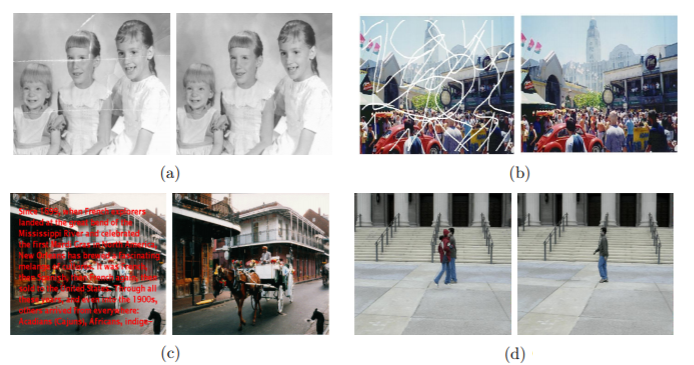
\includegraphics[scale=1.1]{rysunki/fig1}
	\caption{Przykłady obrazów poddanych operacji wmalowywania. Źródło \cite{BertalmioNavierStokes}, \cite{bertalmio2000image} i \cite{patwardhan2007video}.}
	\label{1_fig1}
\end{figure}
\par
Obrazy przedstawiono parami: po lewej obraz wejściowy - uszkodzony i po prawej obraz wynikowy - odrestaurowany. Operacji wmalowywania poddaje się uszkodzone obrazy takie jak (a) i (b), bądź jak (c) obrazy przesłonięte umieszczonymi napisami. Często pożądanym jest usunięcie wybranego obiektu z obrazu tak jak np. w przypadku (d) usunięcie postaci. Przestrzeń do wmalowywania w obrazie wyznaczana jest manualnie poprzez użytkownika definiującego konkretny obiekt, który powinien według użytkownika zostać usunięty. Program automatycznie nie jest w stanie wyznaczyć części, która powinna zostać odrestaurowana. 
Techniki wmalowywania znajdują szeroki zakres zastosowań w przetwarzaniu nagrań filmowych, gdzie nieznany obszar sceny wizyjnej musi zostać oszacowany w pewien sposób dostarczając spójności wizualnej użytkownikowi. Przykładami mogą być konieczność ukrywania błędów nagrań, strat wynikających z błędów urządzeń nagrywających, czy też usunięcia niepożądanych obiektów, które w trakcie nagrywania pojawiły się w kadrze. 
\chapter{Przegląd istniejących algorytmów.}
Pierwszą gałęzią algorytmów zgodnie z rozróżnieniem wprowadzonym w  \cite{SalientStrucTexProp} są metody opierające się na rozwiązaniu równań różniczkowych wyższego rzędu. Wśród nich pojawia się próba przystosowania procesu dyfuzji do wypełniania braków w obrazie (źródła \cite{bertalmio2000image} lub \cite{BertalmioNavierStokes}), dzięki której przy wykorzystaniu zależności z działu mechaniki płynu można dokonać próby kontynuacji informacji z otoczenia w brakujące obszary. \\
Drugą gałęzią algorytmów są metody oparte na uzupełnianiu braków obrazu fragment po fragmencie skopiowanymi częściami istniejącego obrazu z miejsc o najlepszym dopasowaniu w miejsce braku. Pierwszy raz taka metoda syntezy obrazu kopiowanymi kawałkami została zaproponowana w \cite{efros1999texture}. Kolejność wypełniania braków nie jest obojętna i ma znaczny wpływ na ostateczną spójność obrazu. Jedna z najpopularniejszych metod określania priorytetu została przedstawiona w \cite{criminisi2004region}. W literaturze pojawiło się wiele metod minimalizujących zjawisko niespójności w obrazie takich jak np. metoda opisana w  \cite{StructurePropagationManual}. \\
Innym sposobem wyznaczenia braków jest zastosowanie analizy funkcjonalnej definiującej problem minimalizacji energii stanowiącej największą grupę istniejących rozwiązań problemu wmalowywania. 
Jej praktyczne zastosowania można znaleźć np. w \cite{MathematicalModelsforNLTextureInpainting}, \cite{ColorTextureInpaintingNLCTVModel}, czy też \cite{arias2011variational}. W przytoczonych przykładach rozwiązanie problemu minimalizacji stanowi wynik w postaci wmalowanego obrazu. Innym przykładem może być problem minimalizacji zdefiniowany w \cite{SalientStrucTexProp} stanowiący pośredni proces w wypełnianiu obrazu. Tu problem minimalizacji, będący segmentacją obrazu, pozwala oddzielić strukturę i teksturę, pozwalając w następstwie na przeprowadzenie oddzielnej syntezy dwóch zbiorów danych, za pomocą różnych algorytmów. \\
Ostatnią grupą algorytmów jest grupa stanowiąca połączenie powyższych algorytmów. Najprostszym przykładem z tej grupy może algorytm opisany w \cite{NavierStokesAndTexturePropagation}, w którym zaproponowano poprzedzenie procesu wmalowywania segmentacją obrazu. Uzyskaną w procesie segmentacji teksturę uzupełnia się metodą najlepszego dopasowania natomiast strukturę uzyskuje na podstawie równań różniczkowych. Kolejnym przykładem może być publikacja \cite{arias2011variational}, w której autorzy proponują model nielokalny wyznaczający nieznany obszar obrazu wykorzystując rachunek wariacyjny, połączony ze zdefiniowaną metryką wyznaczającą odległości pomiędzy rozpatrywanymi fragmentami obrazu. \\
Większość metod wmalowywania opisanych w literaturze opiera się na algorytmach kontynuujących strukturę, geometrię bądź teksturę obrazu. Modele bazujące na geometrii i strukturze w uogólnieniu generują efekt uboczny w postaci braku kontynuacji tekstur, co sprawia wrażenie rozmytego obrazu. Do algorytmów broniących się przed efektem rozmycia można zaliczyć takie, w których wyznaczeniu konkretnego miejsca w nieznanym obszarze może towarzyszyć przebadanie całego zbioru punktów niemodyfikowanej części obrazu. Stąd metody kontynuujące tekstury w większości uważa się za metody nielokalne.
\chapter{Równania mechaniki płynu.}
\label{chap:navierstokes}
\section{Rozwiązanie równania Naviera-Stokesa }
\label{sec:snavierstokes}
W celu dokładnego zaprezentowania idei wmalowywania w oparciu o równanie Naviera-Stokesa należy rozważyć następujące równanie przepływu cieczy Newtonowskiej:
\begin{equation}
V \nabla V \mathrm{+} \frac{dV}{dt} = - \frac{\mathrm{1}}{q}\nabla p\mathrm{+}F \mathrm{+}\nu {\nabla }^{\mathrm{2}} V
\label{NavierStokesEquation}
,
\end{equation}
\begin{equation}
V = \left( -\frac{\partial\Psi}{\partial y},\frac{\partial \Psi}{\partial x} \right)
\label{LiquidVelociy}
,
\end{equation}
gdzie $V$ oznacza prędkość lokalną, $t$ chwilę czasu, $q$ gęstość lokalną, $p$ ciśnienie lokalne, $F$ siłę zewnętrzną działającą lokalnie na ciecz, $\nu$ lepkość kinematyczną lokalną. $\mathit{\Psi}$ oznacza linię prądu będącą ciągłą linią w polu prędkości płynu, poprowadzoną
stycznie do wektorów prędkości w danej chwili \cite{BertalmioNavierStokes}. Człon $V\nabla V$ odpowiada konwekcji lokalnego pędu wraz z ruchem cieczy, $\frac{1}{q}\nabla p$ wpływowi sił ciśnieniowych na zmianę pędu (kompensuje niezerową konwekcję),  $F$ odpowiada sile zewnętrznej działającej na ciecz (np. grawitację) natomiast $\nu {\nabla }^2V\ $ odpowiada dyssypacji pędu cieczy od tarcia pomiędzy cząstkami. Traktując płyn jako nieściśliwy ($q \leftarrow \infty $)  oraz pomijając działanie sił zewnętrznych ($F=0$)  równanie \eqref{NavierStokesEquation} możemy uprościć do postaci:
\begin{equation}
 V\nabla V+\frac{dV}{dt}=\nu {\nabla }^2V
\label{NavierStokesEquationShort}
.
\end{equation}
Dokonując obustronnej rotacji równania \eqref{NavierStokesEquation} otrzymujemy równanie w zależności od wirowości (zgodnie z \cite{StreamfuntionVorticityForm})
\begin{equation}
V\nabla \omega \mathrm{+}\frac{d\omega }{dt}\mathrm{=}\nu {\nabla }^{\mathrm{2}}V
\label{NavierStokesEquationVorticity}
,
\end{equation}
przy czym wirowość określa się wzorem:
\begin{equation}
\omega =\nabla \times V
\label{Vorticity}
.
\end{equation}
Niech $I$ reprezentuje obraz cyfrowy będący macierzą o rozmiarze $m \mathrm{\times} n$, \cite{ebrahimi2012navier}. Wtedy $I_{i,j}$ zawiera wartość dodatnią całkowitą z przedziału od 0 do 255, stanowiącą informację o poziomie jasności danego piksela z obrazu. Wartość 0 opowiada odcieniowi czarnemu, natomiast 255 odcieniowi czystemu białemu. Niech D stanowi zbiór indeksów $(i,j)\ \in \ \left\{1,2\dots ,m\right\} \mathrm{\times}$ $\left\{1,2\dots ,n\right\}$. Obraz $I$ wtedy można traktować jako funkcję $I:D\to R$. \\
W 2000 roku Bertalmio w \cite{BertalmioNavierStokes} wprowadza analogię pomiędzy wirowością a gładkością obrazu. Dokładniej przedstawia to \autoref{tab1}
\begin{table}[!h]
	\centering
	\begin{tabular}{|cc|c|}
	\hline \hline

		& Navier-Stokes
		& Wmalowywanie w obrazie\\ \hline
		
		& Linia prądu $\ \mathit{\Psi}$ &  Jasność obrazu $I$ \\ \hline
	
		& Prędkość płynu $V = {\mathrm{\nabla }}^{\bot }\mathit{\Psi} = [u, v]$  & Kierunek izotop $V$ = ${\mathrm{\nabla }}^{\bot }I = [u, v]$ \\ \hline
		& Wirowość $\omega =\ {\mathrm{\nabla }}^2\mathit{\Psi}$ & Gładkość $\omega =\ {\mathrm{\nabla }}^2I$ \\ \hline
		
		& Lepkość płynu $\nu $ & Parametr dyfuzji anizotropowej $\nu $ \\
	\hline
	\end{tabular}
	\caption{przekształcenie zmiennych w zagadnieniu wmalowywnia obrazu.}
	\label{tab1}
\end{table}
gdzie ${\nabla }^{\bot }=\left(\frac{\partial }{\partial y},\frac{\partial }{\partial x}\right)$.
Niech $\mathit{\Omega}\subset D$ stanowi wypełniany obszar obrazu (maskę). W wyniku rozwiązania dyskretnego równania Naviera-Stokesa w obszarze maski z warunkami brzegowymi zdefiniowanymi jako jasność pikseli sąsiadujących z obszarem maski uzyskuje się kontynuację linii o podobnej jasności (izolinii) w głąb odrestaurowywanego obszaru zgodnie z \autoref{3_fig1}.  Matematycznie kierunek izolinii jasności obrazu wyznacza ${\nabla }^{\bot }I$. W oparciu o \autoref{tab1} oraz równanie  \eqref{NavierStokesEquationVorticity} wyciągamy wniosek, że zagadnienie wmalowywania można sformułować jako problem stabilnego rozwiązania następującego równania różniczkowego:
\begin{equation}
\left( \nabla ^ \bot I \right) \cdot \nabla \left(\nabla^{2} I \right) +\frac{d\left( \nabla ^{2}I\right)}{\mathrm{d}t} = \nu \nabla \Big[ g \Big( \nabla \left(\nabla ^2 I \right) \Big) \nabla \left( \nabla^2 I \right) \Big]
\label{NavierStokesInpainting}
.
\end{equation}
\begin{figure}[!h]
	\centering
	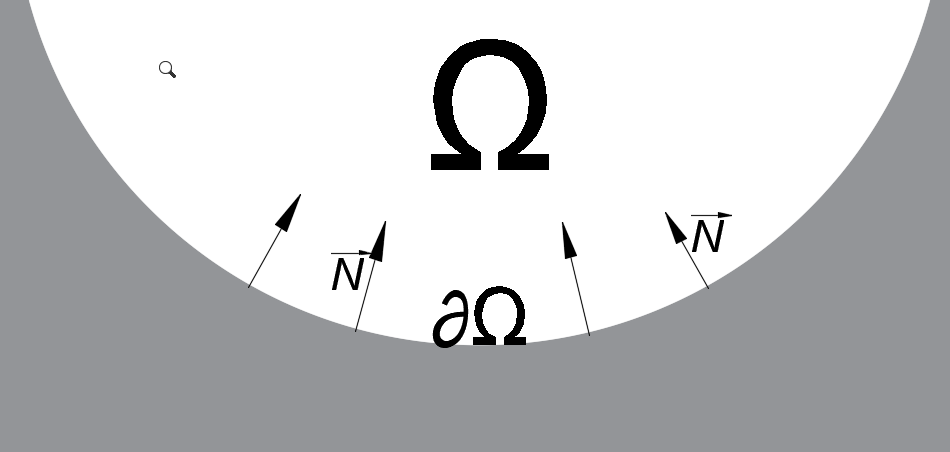
\includegraphics[scale=0.3]{rysunki/3_fig1}
	\caption{Propagacja jasności obrazu wgłąb nieznanego obszaru. Rysunek autorski.}
	\label{3_fig1}
\end{figure}
W równaniu \eqref{NavierStokesInpainting} człon odpowiedzialny za tarcie pomiędzy cząstkami płynu $\nu {\nabla }^2V\ $ został zastąpiony dyfuzją anizotropową, która w kontekście przetwarzania obrazów pierwszy raz wprowadzona została przez Perona i Malika w 1987 roku \cite{perona1990scale}.
Dyfuzja anizotropowa ma znaczny wpływ na zachowanie krawędzi obrazu oraz poprawę jego ostrości. Za dyfuzję anizotropową odpowiada współczynnik $g$, który przedstawiany jest w różnych postaciach funkcji przewodności. W publikacji \cite{au2001image} autorzy wykorzystują postać:
\begin{equation}
g\left(s\right)=\frac{1}{1+\alpha \left|s\right|}
,
\end{equation}
gdzie $\alpha$ oznacza wcześniej zdefiniowane parametry dyfuzji (stałe), ${\mathrm{\nabla }}^{\bot }=({-\partial }_y,{\partial }_x)$. 
Dyskretne rozwiązanie równania \eqref{NavierStokesInpainting} jest analogiczne do dyskretnego rozwiązania przepływu płynu w przestrzeni $2D$. W tym celu należy wprowadzić chwile dyskretne $t=n\cdot \Delta t$, gdzie $n=\left\{1,2,3,\dots ,N\right\}$, $\Delta t$ wartość przyrostu czasu pomiędzy dyskretnymi chwilami $n$ i $n+1$, $N$ moment osiągnięcia stanu ustalonego, matematycznie przedstawianego jako:
\begin{equation}
\frac{\partial I}{\partial t}\mathrm{+}{\mathrm{\nabla }}^{\mathrm{\bot }}I\mathrm{\nabla }\mathrm{\Delta }I\mathrm{\ }\mathrm{\cong }\mathrm{0}
\label{NavierStokesStability}
.
\end{equation}
Warto zauważyć, że człon ${\mathrm{\nabla }}^{\bot }I$ w równaniu \eqref{NavierStokesStability} odpowiada kierunkowi linii tworzonej przez punkty o podobnej jasności, natomiast $\mathrm{\nabla }\Delta I$ to kierunek największej zmiany gładkości obrazu. Jeśli wektory są do siebie prostopadłe to iloczyn skalarny wynosi 0 i przedstawia stan stabilny. 
W celu dokładnej analizy dyskretyzacji równanie \eqref{NavierStokesEquationVorticity} zostanie rozdzielone na dwa podrównania:
\begin{equation}
\frac{\mathrm{d}{\mathrm{(}\mathrm{\nabla }}^2I)}{\mathrm{d}t}=-{\mathrm{(}\mathrm{\nabla }}^{\bot }I)\cdot \nabla {\mathrm{(}\mathrm{\nabla }}^2I)+\left\{ad\right\}
\label{NavierDiffAdv}
,
\end{equation}
\begin{equation}
{ad}=\nu \nabla \Big[ \nabla 
\Big(\mathrm{\nabla }^2I)\Big)\nabla {\mathrm{(}\mathrm{\nabla }}^2I)\Big]
\label{NavierAdv}
.
\end{equation}
Rozwiązanie powyższych równań dokonywane będzie na siatce obliczeniowej typu Eulera, a wszystkie wartości wyznaczanych zmiennych będą znajdować się w centrach komórek zdefiniowanych jako konkretne piksele obrazu.
\begin{longtable}{ ||P{2cm}|P{2cm}|P{2cm}|| } 
 \hline \hline
 $i-1, j-1$ & $i-1, j$ & $i-1, j+1$ \\ \hline
 $i, j-1$ & $i, j$ & $i, j+1$ \\ \hline
 $i+1, j+1$ & $i+1, j$ & $i+1, j+1$ \\ \hline \hline
\caption{Widok siatki obliczeniowej typu Eulera.}
\end{longtable}
Równanie \eqref{NavierDiffAdv} to równanie różniczkowe cząstkowe typu parabolicznego. Równanie to  można rozwiązać w sposób przybliżony używając schematu różnicy centralnej bądź schematu różnicy do przodu. W przypadku równania parabolicznego oba schematy dają stabilne rozwiązanie. W celu ułatwienia dalszych rozważań wprowadzono funkcję $f$ określoną w centrach siatki, z dolnymi indeksami wskazującymi na konkretne miejsce w siatce. Korzystając z rozwinięcia w szereg Taylora możemy gradient funkcji $f$ w punkcie $(i,j)$ przybliżyć następującym wzorem:
\begin{equation}
\nabla f_{i,j}=\left[\ {\frac{\partial f}{\partial x}\bigg |}_{i,j,} \ {\frac{\partial f}{\partial y}\bigg |}_{i,j}\right]
\label{gradF}
,
\end{equation}
gdzie:
\begin{equation}
{\frac{\partial f}{\partial x}} {\bigg |}_{i,j}=\frac{f_{i+1,j}+f_{i-1,j}}{2\Delta x}
\label{dfdx}
,
\end{equation}
\begin{equation}
{\frac{\partial f}{\partial y}} {\bigg |}_{i,j}=\frac{f_{i,j+1}+f_{i,j-1}}{2\Delta y}
\label{dfdy}
.
\end{equation}
Na podstawie wzorów \eqref{gradF} - \eqref{dfdy} składowe wektora ${\mathrm{\nabla }}^{\bot }I$, czyli kierunku, w którym należy propagować gładkość obrazu ${\mathrm{\nabla }}^2I$ wyznacza się z zależności:
\begin{equation}
u_{i,j}=\frac{I_{i,j+1}+I_{i,j-1}}{2\Delta y} 
\label{u}
,
\end{equation}
\begin{equation}
 v_{i,j}=-\frac{I_{i+1,j}+I_{i-1,j}}{2\Delta x}
\label{v}
,
\end{equation}
przy czym:
\begin{equation}\\
{\mathrm{\nabla }}^{\bot }I=\left[-u,v\right]
\label{gradI}
.
\end{equation}
Jeśli zastosujemy pięciopunktowy analog różnicowy \cite{blacksuccessive} w metodzie różnic skończonych to operator Laplace’a dla przyjętej siatki Eulera można przybliżyć następującym wzorem (przy założeniu, że $\Delta x=\ \Delta y$):
\begin{align}
\begin{aligned}
{\mathrm{\nabla }}^2f_{i,j} &= \Delta f_{i,j}=\\[1ex]
&={\frac{{\partial }^2f}{\partial x^2}}\bigg|_{i,j}+{\frac{{\partial }^2f}{\partial y^2}}\bigg|_{i,j}=\\
&=\frac{f_{i+1,j+1}+f_{i-1,j+1}+f_{i+1,j-1}+f_{i-1,j-1}-4f_{i,j}}{\Delta x^2} .
\end{aligned}
\label{LaplaceOpr}
\end{align}
Jeśli skorzystamy z wyznaczonych wcześniej zależności na wartości $u$ oraz $v$ to wartość gładkości obrazu $\omega =\ {\mathrm{\nabla }}^2I$ można przedstawić w postaci: 
\begin{equation}
\Delta {I}\big|_{i,j}=\ {\frac{\partial v}{\partial x}}\bigg|_{i,j,}-\ {\frac{\partial u}{\partial y}}\bigg|_{i,j}
\label{discreteVorticity}
.
\end{equation}
Podobnie jak w przypadku liczenia pochodnej w dziedzinie obrazu pierwszą pochodną w dziedzinie czasu przybliża się rozwinięciem w szereg Taylora. Niech indeks górny oznacza konkretną chwilę czasową. Wtedy wartość pochodnej wynosi:
\begin{equation}
\ {{\frac{\partial f}{\partial t}}\bigg|^n_{i,j}=\ \frac{f^{n+1}_{i,j}-\ f^n_{i,j}}{\Delta t}}
\label{dfdt}
.
\end{equation}
Ostatecznie rozwiązanie dyskretnego równania parabolicznego \eqref{NavierDiffAdv} , gdzie $\Delta x= \Delta y=h$, z wykorzystaniem \textbf{schematu centralnego} ma postać:
\begin{align}
\omega ^{n+1}_{i,j} &= {\omega }^n_{i,j} - \frac{\Delta t}{4h^2}\biggl[u_{i,j} \left({\omega }_{i+1,j}
-{\omega }_{i-1,j}\right)+ v_{i,j} \left({\omega }_{i,j+1}+{\omega }_{i,j-1}\right)\biggr]+\notag\\ 
&\qquad + \Delta t{\left\{ad\right\}}_{i,j}.
\label{NavierDiffAdvCen}
\end{align}
Rozwiązanie równania \eqref{NavierDiffAdv} można przedstawić również w drugiej postaci wykorzystującej schemat „\textbf{do przodu}”, charakteryzujący się wyznaczaniem wartości pochodnej wirowości w zależności od wyznaczonego kierunku ${\mathrm{(}\mathrm{\nabla }}^{\bot }I)$.  Wtedy równanie \eqref{NavierDiffAdvCen} przyjmuje postać:
\begin{align}
\fontsize{11} \omega
\omega^{n+1}_{i,j} &= {\omega }^n_{i,j} - \frac{\Delta t}{4h^2}\biggl[\left|u_{i,j}\right|
\left({\omega }_{k,j}+{\omega }_{i,j}\right)+
\left|v_{i,j}\right| \left({\omega }_{i,l}+{\omega }_{i,j}\right) \biggr] + \notag\\ 
&\qquad+ \Delta t {\left\{ad\right\}}_{i,j},
\label{NavierDiffAdvFor}
\end{align}
gdzie:
\begin{align}
k = i+sgn\left(u^n\right), \\
l = j+sgn(u^n).
\end{align}
Rozwiązanie równania \eqref{NavierAdv}, w którym zastąpiono postać zwykłej dyfuzji przez wyrażenie $\nu {\nabla }^2V$ wymaga uważniejszego potraktowania ze względu na większą podatność na niestabilność implementowanych metod dyskretyzacji. Równanie to można przedstawić w postaci dywergencji pola wektorowego uzyskanego w wyniku wyliczenia gradientu wirowości z uwzględnionym współczynnikiem dyfuzji anizotropowej:
\begin{align}
\begin{aligned}
\left\{ad\right\} 
&= \nu \nabla\Big[g\Big(\nabla {(\mathrm{\nabla }}^2I)\Big)\nabla {\mathrm{(}\mathrm{\nabla }}^2I)\Big]= \\[1ex]
&= \nu \nabla \cdot \Big[g\big(|\nabla \omega|\big)\nabla \omega \Big]=\\[1ex]
&= \partial _x \Big(g\big(\left|\nabla \omega \right|\big){\partial }_x\omega \Big)+ \partial_y \Big(g\big(\left|\nabla \omega \right|\big){\partial }_y\omega \Big),
\end{aligned}
\label{Anisotropic}
\end{align}
gdzie: ${\partial }_x=\frac{\partial }{\partial x}$ oraz analogicznie: ${\partial }_y=\frac{\partial }{\partial y}$.
Zgodnie z \cite{ebrahimi2012navier} równanie można rozwiązać w następujących krokach:
Korzystając z zależności \eqref{dfdx} i \eqref{dfdy} należy wyznaczyć wartości ${\frac{d\omega }{dx}}\big|_{i,j}$ oraz ${\frac{d\omega }{dy}}\big|_{i,j}$
Korzystając z obliczonych wartości należy następnie obliczyć moduł wektora w przestrzeni Euklidesowej:
\begin{equation}
{\left|\mathrm{\nabla }\omega \right|}_{i,j}=\ \sqrt{\frac{\partial \omega }{\partial x}\bigg|^2_{i,j}+\frac{\partial \omega }{\partial y}\bigg|^2_{i,j}}
\label{magnitudedw}
.
\end{equation}
Na podstawie wyznaczonego modułu należy obliczyć wartość $g{\left({\left|\mathrm{\nabla }\omega \right|}_{i,j}\right)}$ wykorzystując \eqref{NavierStokesInpainting}. Korzystając z wartości wyznaczonych wcześniej oraz ponownie z zależności \eqref{dfdx} i \eqref{dfdy} możemy wyliczyć wartość $\{ad_{i,j}\} $:
\begin{align}
\{ad_{i,j}\} &= \partial_x \left( g(\left| \nabla\omega \right|_{i,j}) \cdot \partial_x \omega \big|_{i,j} \right) \bigg|_{i,j} \notag +\\[1ex]
&+ \partial_y \left( g(\left|\nabla\omega\right|_{i,j}) \cdot \partial_y \omega \big|_{i,j} \right)\bigg|_{i,j}.
\label{discreteAnisotropic}
\end{align}
Należy zauważyć, iż do wyznaczenia wartości $u$, $v$ oraz ${\mathrm{\nabla }}^2I$ wykorzystywanych do obliczeń \eqref{NavierDiffAdv} i \eqref{NavierAdv} w każdej kolejnej chwili czasu (iteracji) $n$, konieczna jest znajomość obrazu $I^n$. W związku z tym równocześnie z równaniem \eqref{NavierDiffAdv} należy rozwiązywać następujące niejednorodne równanie różniczkowe cząstkowe liniowe drugiego rzędu.
\begin{equation}
\Delta I^n={\omega }^n
\label{Poisson}
.
\end{equation}
Dla przestrzeni dwuwymiarowej równanie to przyjmuje następującą postać:
\begin{equation}
\frac{{{\partial }^2I}^n}{\partial x^2}+\frac{{{\partial }^2I}^n}{\partial y^2}=\ \omega^n
\label{Poisson2D}
.
\end{equation}
Aproksymacje pochodnych cząstkowych drugiego stopnia schematem centralnym przedstawiają następujące zależności:
\begin{equation}
{\frac{{\partial }^2f}{\partial x^2}\bigg|}_{i,j}\mathrm{=}\frac{f_{i+1,j}-2f_{i,j}+f_{i-1,j}}{\Delta x^2}
\label{d2fdx2}
,
\end{equation}
\begin{equation}
{\frac{{\partial }^2f}{\partial y^2}\bigg|}_{i,j}\mathrm{=}\frac{f_{i,j+1}-2f_{i,j}+f_{i,j-1}}{\Delta y^2}
\label{d2fdy2}
.
\end{equation}
Jeśli skorzystamy z zależności \eqref{d2fdx2} oraz \eqref{d2fdy2} to równanie \eqref{Poisson} w punkcie $(i,j)$ przyjmuje postać pięciopunktowego analogu różnicowego operatora $\Delta $ ($\Delta x=\ \Delta y=h)$:
\begin{equation}
I_{i+1,j}+I_{i-1,j}+I_{i,j+1}+I_{i,j-1}-4I_{i,j}=h^2{\omega }_{i,j}
\label{Laplace}
.
\end{equation}
Na podstawie równania \eqref{Laplace} można stworzyć równanie macierzowe postaci $Ax=B$, gdzie $x$ reprezentuje nasz obraz $I$, $B$ gładkość obrazu $\omega$, natomiast $A$ to macierz charakterystyczna współczynników. Istnieje wiele różnych metod rozwiązywania równań Poissona takich jak metoda Jacobiego czy Gauss'a-Seidla.  Wystarczającą wydajność i szybkość działania w celach rozwiązania równania można uzyskać stosując podejście SOR – czyli metodę sukcesywnej nadrelaksacji, \cite{blacksuccessive}. Dyskretyzacja równania wygląda następująco:
\begin{align}
\begin{aligned}
I^{n+1}_{i,j}
&= \left(1-\ \beta \right)I^n_{i,j}+\beta \cdot \frac{1}{2}{\left(\frac{1}{\Delta x^2}+\frac{1}{\Delta y^2}\right)}^{-1} \cdot \\[1ex]
&\cdot \left[\frac{1}{\Delta x^2}{(I}^n_{i+1,j}+I^{n+1}_{i-1,j})+\frac{1}{\Delta y^2}{(I}^n_{i,j+1}+I^{n+1}_{i,j-1})+{\omega }^n_{i,j}\right]
\end{aligned}
\label{DiscreteSOR}
\end{align}
Metoda ta w swoim równaniu ma parametr wagowy $\beta$ odpowiadający za zbieżność algorytmu i musi on zawierać się w przedziale $(0,2)$ \cite{neumann1981kahan}. Według informacji podanych w  \cite{blacksuccessive} parametr ten powinno przyjmować się zgodnie z zależnością:
\begin{equation}
{\omega }_{opt}=2{\left(1+\frac{\pi }{N}\right)}^{-1}
\label{BetaChoose}
.
\end{equation}
gdzie $N$ to liczba kolumn przyjętej siatki obliczeniowej. 
\par
Operacje wmalowywania bardzo często wykonywane są w punktach maski tworzących nieregularne kształty, mogących znajdować się w różnych częściach obrazu. Dlatego też wcześniej przedstawiony schemat obliczeń wykonywany jest dla wszystkich pikseli obrazu. Po każdej iteracji uzyskane wartości $I^{n+1}$ w znanych punktach przepisywane są z oryginalnego obrazu $I^{0}$, zgodnie z zależnością:
\begin{equation}
I^{n+1}(D/\mathrm{\Omega }\mathrm{)\ }\ ={\ I}^0(D/\mathrm{\Omega }\mathrm{)}.
\label{retrieveMask}
\end{equation}
Podsumowując, w celu wyznaczenia nieznanych wartości obrazu w punktach zdefiniowanych przez maskę należy powtarzać następujące kroki do uzyskania stanu ustalonego:
\begin{enumerate}
\item
Rozwiązać równanie \eqref{discreteAnisotropic}.
\item
Na podstawie równania \eqref{NavierDiffAdvCen} zamiennie z \eqref{NavierDiffAdvFor} wyznaczyć wartości $\omega_{i,j}^{n+1}$ dla każdego punktu $(i,j)$.
\item
Korzystając z \eqref{DiscreteSOR} wyznaczyć jasność każdego piksela $I_{i,j}^{n+1}$.
\item
Do uzyskanego obrazu w punkcie 3 przepisać znane wartości z obrazu oryginalnego.
\end{enumerate}
Powyższy algorytm przedstawiono dla obrazów w odcieniach szarości $I:D\to R$. W przypadku obrazów kolorowych, zdefiniowanych funkcją będącą przekształceniem w pole wektorowe $[R,G,B]$, czyli $I:D\to R^3$ metodę stosuje się oddzielnie dla każdej warstwy. Zgodnie z propozycją przedstawioną w \cite{fishelov2006image} obraz można również przekształcić w poprzedzającym algorytm kroku do współrzędnych sferycznych (CIELab) $\left[I_{1},I_{2},I_{3} \right]$ zgodnie z zależnościami:
\begin{equation}
{I_{1_{i,j}}=r}_{i,j}=\ \sqrt{R^2_{i,j}+G^2_{i,j}+B^2_{i,j}}
\label{TIone}
,
\end{equation}
\begin{equation}
I_{2_{i,j}}=\ {\mathrm{sin} {\mathrm{\Theta }}_{i,j}\ }=\ {\mathrm{sin} {{\mathrm{tan}}^{-1} \frac{G_{i,j}}{R_{i,j}}\ }\ } 
\label{TItwo}
,
\end{equation}
\begin{equation}
I_{3_{i,j}}=\ {\mathrm{sin} {\phi }_{i,j}\ }=\ {\mathrm{sin} {{\mathrm{cos}}^{-1} \frac{B_{i,j}}{r_{i,j}}\ }\ } 
\label{TIthree}
.
\end{equation}
Następnie dysponując składowymi $I_1$, $I_2$, $I_3$ wyznaczonymi z powyższych zależności, dla każdego z nich oddzielnie wykonujemy wcześniej opisane iteracje. W celu wykonania odwrotnego przekształcenia $\left[I_1,I_2,I_3 \right]\to\left[R,G,B\right]$ wystarczy przeprowadzić następujące obliczenia:
\begin{equation}
 B_{i,j}=\ r_{i,j}{\mathrm{cos} {\mathrm{\Theta }}_{\mathrm{i,j}}\ }{\mathrm{cos} {\phi }_{\mathrm{i,j}}\ }
\label{TInvIone}
,
\end{equation}
\begin{equation}
R_{i,j}=\ r_{i,j}{\mathrm{cos} {\mathrm{\Theta }}_{\mathrm{i,j}}\ }{\mathrm{sin} {\phi }_{\mathrm{i,j}}\ }
\label{TInvItwo},
\end{equation}
\begin{equation}
G_{i,j}=\ r_{i,j}{\mathrm{sin} {\theta }_{\mathrm{i,j}}\ } 
\label{TInvIthree}
.
\end{equation}
Operację wmalowywania można wykonać na pierwotnych składowych $[R,G,B]$ lecz matematyczna transformacja przestrzeni charakteryzuje się lepszymi właściwościami związanymi z postrzeganiem różnicy barw $\delta E$ przez ludzkie oko:
\begin{equation}
\Delta E=\ \sqrt{{\Delta I_1}^2+{\Delta I_2}^2+{\Delta I_3}^2}
\label{deltaE}
.
\end{equation}
\chapter{Metody oparte na procesie minimalizacji energii.}
\section{Segmentacja obrazu na strukturę i teksturę.}\label{sec:StructureTextureNavierStokes}
Metoda jednoczesnego wmalowywania struktur i tekstur pierwszy raz przedstawiona została przez Bertalmio w 2003 roku w \cite{NavierStokesAndTexturePropagation}. Opiera się ona na wmalowywaniu struktury w oparciu o algorytm przedstawiony w artykule przy jednoczesnej propozycji prostej syntezy tekstury. Niech $I$ oznacza obraz $R^2\to R,\ \ I\in L^2(R^2)$. Proces wypełniania brakującego regionu $\mathrm{\Omega }$ poprzedzony jest dekompozycją obrazu:
\begin{align}
I\left(i,j\right)=u\left(i,j\right)+v\left(i,j\right).
\label{STRUCTURETEXTURE1}
\end{align}
uzyskaną na podstawie rozwiązania problemu minimalizacji energii:
\begin{align} 
{\mathop{\mathrm{min}}_{u} \Biggl\{E\left(u\right)=\int{\left|\mathrm{\nabla }u\right|+\lambda {\left|\left|v\right|\right|}^2_{L^2}}\Biggr\}\ },
\label{STRUCTURETEXTURE2}
\end{align}
gdzie: $\int{\left|\mathrm{\nabla }u\right|}$ stanowi funkcjonał z przestrzeni o wariacji ograniczonej oznaczanej $BV(R^2)$ pozwalający usunąć z oryginalnego obrazu szum i teksturę przy jednoczesnym zachowaniu głównych cech oraz ostrych krawędzi, ${\left|\left|v\right|\right|}^2_{L^2}$ to człon odpowiadający za dokładność odwzorowania, a $\lambda $ stanowi wcześniej zdefiniowany parametr. Zgodnie z dowodem Mayera \cite{meyer2001oscillating} dla odpowiednio małych wartości $\lambda $ problem minimalizacji prowadzi do uzyskania składowej zmiennej $u$ reprezentującej odfiltrowany obraz oraz składowej zmiennej $v$ reprezentującej szumy i tekstury obrazu. Nasz problem segmentacji można przedstawić jako zagadnienie minimalizacji energii \cite{vese2003modeling}:
\begin{align}
\begin{aligned} 
\mathop{\mathrm{min}}_{u,g_1,g_2} \Biggl\{E &= \int{\left|\mathrm{\nabla }u\right| } \ + \\
&+\lambda \int{\left|I-u-\partial_x g_1- \partial_y g_2 \right|}^2dxdy \ +\\
&+ \mu {\left[\int{{\sqrt{g^2_1+g^2_2}}^\beta dxdy}\right]}^{\frac{1}{\beta}}\Biggr\},
\end{aligned}
\end{align}
gdzie:
\begin{align}
v=div(g),\ g=\left[ g_1,g_2 \right],\ g_1=-\frac{1}{2\lambda }\frac{u_x}{\left|\mathrm{\nabla }u\right|},\ g_2=-\frac{1}{2\lambda }\frac{u_y}{\left|\mathrm{\nabla }u\right|}.
\label{VG1G2}
\end{align}
Minimalizacja względem $u, g_1$ i $g_2$ w rezultacie prowadzi do równań Eulera-Lagrange'a \cite{vese2003modeling}:
\begin{align}
u=I-{\partial }_xg_1-{\partial }_yg_2+\frac{1}{2\lambda }div\left(\frac{\mathrm{\nabla }u}{\left|\mathrm{\nabla }u\right|}\right),
\label{EL1}
\end{align}
\begin{align}
{\mu H\left(g_1,g_2\right)g}_1=2\lambda \left[\frac{\partial }{{\partial }_x}\left(u-I\right)+{\partial }^2_{xx}g_1+{\partial }^2_{xy}g_2\right],
\label{EL2}
\end{align}
\begin{align}
\mu H\left(g_1,g_2\right)g_2=2\lambda \left[\frac{\partial }{{\partial }_y}\left(u-I\right)+{\partial }^2_{xy}g_1+{\partial }^2_{yy}g_2\right].
\label{EL3}
\end{align}
gdzie $\mu$ stanowi predefiniowany parametr dyskretyzacji, natomiast $H\left(g_1,g_2\right)$ opisane jest wzorem:
\begin{align}
H\left(g_1,g_2\right)=\frac{1}{\sqrt{g^2_1+g^2_2}}.
\end{align}
Formalnie, równanie Eulera-Lagrange'a uzyskane podczas minimalizacji energii \eqref{STRUCTURETEXTURE2} przyjmuje postać \cite{vese2003modeling}:
\begin{align}
u=I+\frac{1}{2\lambda }div\left(\frac{\mathrm{\nabla }u}{\left|\mathrm{\nabla }u\right|}\right).
\label{uToInsert}
\end{align}
Pamiętając, że $v = I -u$ podstawiając w miejsce $u$ zależność \eqref{uToInsert} otrzymujemy zależność
\begin{align}
v=-\frac{1}{2\lambda }div\left(\frac{\mathrm{\nabla }u}{\left|\mathrm{\nabla }u\right|}\right).
\end{align}
Korzystając z zależności \eqref{VG1G2} możemy łatwo zauważyć, że:
\begin{align}
\begin{aligned}
g^2_1+g^2_2 & = 
\left(-\frac{1}{2\lambda }\frac{u_x}{\left|\mathrm{\nabla }u\right|}\right)^2 +  \left(-\frac{1}{2\lambda }\frac{u_y}{\left|\mathrm{\nabla }u\right|}\right)^2 &=\\
&= \frac{1}{2\lambda} \frac{u_x^2 + u_y^2 }{|\nabla u|^2} = \frac{1}{2\lambda} \frac{|\nabla u|^2}{|\nabla u|^2} = \frac{1}{2\lambda}.
\end{aligned}
\end{align}
Stąd:
\begin{align}
H\left(g_1,g_2\right)=\frac{1}{\sqrt{g^2_1+g^2_2}} = \frac{1}{\sqrt{\frac{1}{2\lambda}}} = \sqrt{2\lambda}.
\end{align}
Zatem równania \eqref{EL1}, \eqref{EL2} i \eqref{EL3} przyjmą postać: 
\begin{align}
u=I-u-{\partial }_xg_1-{\partial }_yg_2+\frac{1}{2\lambda }div\left(\frac{\mathrm{\nabla }u}{\left|\mathrm{\nabla }u\right|}\right),
\label{EU}
\end{align}
\begin{align}
\mu \sqrt{2\lambda }g_1=2\lambda \left[\frac{\partial }{{\partial }_x}\left(u-I\right)+{\partial }^2_{xx}g_1+{\partial }^2_{xy}g_2\right],
\label{EG1}
\end{align}
\begin{align}
\mu \sqrt{2\lambda }g_2=2\lambda \left[\frac{\partial }{{\partial }_y}\left(u-I\right)+{\partial }^2_{xy}g_1+{\partial }^2_{yy}g_2\right]
\label{EG2}.
\end{align}
Jako wartości początkowe tego iteracyjnego algorytmu można przyjąć:
\begin{align}
u^0=f,\ g_1=-\frac{1}{2\lambda }\frac{f_{\mathrm{x}}}{\left|\mathrm{\nabla }f\right|},\ g_2=-\frac{1}{2\lambda }\frac{f_{\mathrm{y}}}{\left|\mathrm{\nabla }f\right|}.
\end{align}
Zgodnie z dokładnym wyprowadzeniem przedstawionym w \cite{vese2003modeling} ostatecznie otrzymujemy:
\begin{align}
\begin{aligned} 
{\partial }_{xy}g_1 \big|_{i,j} &\cong \frac{1}{2h^2} \bigg[2g_1\big|_{i,j}+g_1\big|_{i-1,j-1}+g_1\big|_{i+1,j+1}-g_1\big|_{i,\ j-1} -\\ 
&-g_1\big|_{i-1,j}-g_1\big|_{i+1,j}-g_1\big|_{i,j+1}\bigg],
\end{aligned}
\end{align}
możemy przedstawić równania \eqref{EU}, \eqref{EG1} i \eqref{EG2} w następującej postaci dyskretnej:
\begin{align}
\begin{aligned}
u^{n+1}\big|_{i,j} &= \left[\frac{1}{1 + \left(\frac{1}{2\lambda h^2}\right)\cdot \left(c_1\big|_{i,j}+c_2\big|_{i,j}+c_3\big|_{i,j}+c_4\big|_{i,j}\right)}\right]\bigcdot \\ 
&\bigcdot \biggl[I\big|_{i,j}- \left(\frac{g^n_1\big|_{i+1,j} - g^n_1\big|_{i-1,j}}{2h}\right)- \left(\frac{g^n_2\big|_{i,j+1}-g^n_2\big|_{i,j-1}}{2h}\right) +\\ 
&+\ \left(\frac{1}{2\lambda h^2}\right)\bigcdot \Bigl[c_1\big|_{i,j}\cdot u^n\big|_{i+1,j}+c_2\big|_{i,j}\cdot u^n\big|_{i-1,j} +\\
&+c_3\big|_{i,j}\cdot \lambda \cdot {u}^n\big|_{i,j+1}+c_4\big|_{i,j}\cdot u^n\big|_{i,j-1}\Bigr]\biggr],
\end{aligned}
\end{align}
\begin{align}
\begin{aligned}
g^{n+1}_1\big|_{i,j} &= \left[\frac{2\lambda }{\mu \sqrt{2\lambda }+\ 4\frac{\lambda }{2h}}\right]\bigcdot \Biggl[\frac{u^n\big|_{i+1,j}-u^n\big|_{i-1,j}}{2h}-\frac{I\big|_{i+1,j}-I\big|_{i-1,j}}{2h}+\\
&+\frac{g_1\big|_{i+1,j}+g_1\big|_{i-1,j}}{h^2}\frac{1}{2h^2}\cdot \Bigl[2g^n_2\big|_{i,j}+ g^n_2\big|_{i-1,j-1} +\\ 
&+ g^n_2\big|_{i+1,j+1}+
g^n_2\big|_{i,j-1}-g^n_2\big|_{i-1,j}+g^n_2\big|_{i+1,j}-\\
&-g^n_2\big|_{i,j+1}\Bigr]\Biggr],
\end{aligned}
\end{align}
\begin{align}
\begin{aligned}
g^{n+1}_2|_{i,j} &=\left[\frac{2\lambda }{\mu \sqrt{2\lambda }\ +\ 4\frac{\lambda }{2h}}\right]\bigcdot \Biggl[\frac{u^n\big|_{i,j+1}-u^n\big|_{i,j-1}}{2h}-\frac{I\big|_{i,j+1}-I\big|_{i,j-1}}{2h}+\\ 
&+\frac{g_2\big|_{i,j+1}+g_2\big|_{i,j-1}}{h^2}+\frac{1}{2h^2}\cdot \Bigl[2g^n_1\big|_{i,j}+ g^n_1\big|_{i-1,j-1}+ g^n_1\big|_{i+1,j+1} -\\
&-\ g^n_1\big|_{i,j-1}-g^n_1\big|_{i-1,j}+g^n_1\big|_{i+1,j}- g^n_1\big|_{i,j+1}\Bigr]\Biggr],
\end{aligned}
\end{align}
przy czym:
\begin{large}
\begin{align}
\begin{aligned}
c^n_1\big|_{i,j}=\frac{1}{\sqrt{{\left(\frac{u^n\big|_{i+1,j}-u^n\big|_{i,j}}{h}\right)}^2+ {\left(\frac{u^n\big|_{i,j+1}-u^n\big|_{i,j-1}}{2h}\right)}^2+\ \varepsilon }},
\end{aligned}
\end{align}
\begin{align}
\begin{aligned}
c^n_2\big|_{i,j}=\frac{1}{\sqrt{{\left(\frac{u^n\big|_{i,j}-u^n\big|_{i-1,j}}{h}\right)}^2+ {\left(\frac{u^n\big|_{i-1,j+1}-u^n\big|_{i-1,j-1}}{2h}\right)}^2+\ \varepsilon }},
\end{aligned}
\end{align}
\begin{align}
\begin{aligned}
c^n_3\big|_{i,j}=\frac{1}{\sqrt{{\left(\frac{u^n\big|_{i+1,j}-u^n\big|_{i-1,j}}{2h}\right)}^2+\ {\left(\frac{u^n\big|_{i,j+1}-u^n\big|_{i,j}}{h}\right)}^2+\ \varepsilon }},
\end{aligned}
\end{align}
\begin{align}
\begin{aligned}
c^n_4\big|_{i,j}=\frac{1}{\sqrt{{\left(\frac{u^n\big|_{i+1,j-1}-u^n\big|_{i-1,j-1}}{2h}\right)}^2+\ {\left(\frac{u^n\big|_{i,j}-u^n\big|_{i,j-1}}{h}\right)}^2+\ \varepsilon }}.
\end{aligned}
\end{align}
\end{large}
W celu uniknięcia problemu dzielenia przez zero w przedstawionej dyskretyzacji wprowadzono parametr $\varepsilon \rightarrow 0$. 
Po przeprowadzeniu takiej segmentacji obrazu dla uzyskanych członów $u$ i $v$ można zastosować różne algorytmy wmalowywania braków. Autorzy w \cite{NavierStokesAndTexturePropagation} proponują aby do wmalowywania struktur zastosować algorytm przedstawiony w \cite{bertalmio2000image}, natomiast do uzyskania brakującej tekstury sugerują użycie następującego algorytmu syntezy obszaru $\mathrm{\Omega }$.
\begin{figure}[!h]
	\centering
	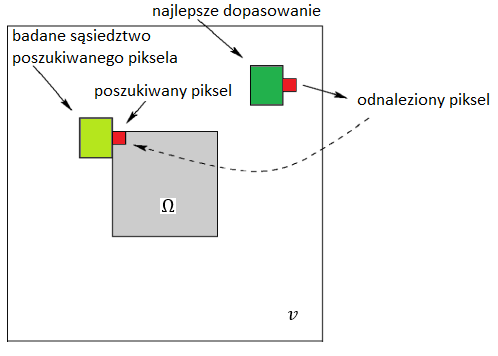
\includegraphics[scale=0.9]{rysunki/5_fig1}
	\caption{Prosty algorytm wmalowywania tekstury obrazu. Rysunek autorski.}
	\label{5_fig1}
\end{figure} \\
Zgodnie z \autoref{5_fig1} dla każdego piksela znajdującego się na granicy obszaru $\mathrm{\Omega }$ tworzone jest okno stanowiące szablon wykorzystywany do odnalezienia najlepszego dopasowania z pośród całego obrazu $v$. W przypadku odnalezienia takiego dopasowania uzyskany piksel kopiowany jest w miejsce piksela brakującego. Algorytm ten można wykonywać pobierając piksele z granicy w kolejności zgodnej z kolejnością obrotu wskazówek zegara, postępując w głąb obszaru $\mathrm{\Omega }$, aż do wypełnienia wszystkich brakujących pikseli. 
W przypadku obrazów kolorowych $I$ w przestrzeni $[R, G, B]$ wypełnianie można poprzedzić wykonaniem przekształcenia $I$ zgodnie z zależnościami \eqref{TIone}, \eqref{TItwo} i \eqref{TIthree}. Następnie każda z trzech uzyskanych warstw jest rozbijana na własną teksturę i strukturę. Kroki tego  algorytmu można przedstawić następująco:
\begin{enumerate}
\item
(Opcjonalnie) Przekształcenie warstw $R,G,B$ obrazu na współrzędne sferyczne $I_1,I_2,I_3$.
\item
Wyznaczenie $u_1,v_1,\ u_2,v_2,u_3,v_3$ na podstawie $I_1, I_2, I_3$, bądź pierwotnych warstw $R, G, B$.
\item
Wmalowanie nieznanych obszarów $\mathrm{\Omega }$ w warstwach $u_1,u_2,u_3$ dowolnie dobraną metodą.
\item
Wmalowanie obszaru $\mathrm{\Omega }$ w $v_1,v_2,v_3$ na podstawie dowolnego algorytmu syntezy tekstury $v_1$.
\end{enumerate}
\textbf{W niniejszej pracy magisterskiej do wypełnienia $u$ posłużono się mętodą Naviera-Stokes'a, natomiast do wypełnienia $v$ metodą Criminisi opisaną w rozdziale \ref{sec:crimMetod}}.
\section{Model nielokalny NLCTV. (Non-local color total variation)}
\subsection{Opis zaproponowanego rozwiązania.}
\label{sec:sNLCTV}
Pojęcie wariacji całkowitej funkcji $TV$ (total variation) w analizie obrazów pierwszy raz wprowadzone zostało przez Rudin'a, Osher'a i Fatemi’ego w \cite{rudin1992nonlinear}, gdzie proponowany model znajduje zastosowanie w usuwaniu szumów z obrazu. Następnie model $TV$ zostaje zaproponowany do wmalowywania obrazu w \cite{MathematicalModelsforNLTextureInpainting} przez Chan'a i Shen’a. Problem doboru parametrów dla modelu $TV$, właściwości oraz proces dyskretyzacji problemu minimalizacji jest dokładnie przedstawiony w \cite{getreuer2012total}. Algorytm bazujący na lokalnych funkcjonałach $TV$  charakteryzuje się zdolnością do kontynuacji geometrycznych struktur obrazu i krawędzi. Zgodnie z przedstawioną literaturą wadą algorytmu jest brak możliwości propagacji tekstury w nieznany obszar $\Omega$. Warto wspomnieć, iż w przypadku usuwania szumów z obrazów wykorzystanie operatorów lokalnych nie pozwala zachować tekstur. Problem jednoczesnej propagacji geometrii i tekstury można rozwiązać przy zastosowaniu modelu nielokalnego, który zostanie poddany analizie w niniejszej pracy. \\
Klasyczny model nielokalny wariacji całkowitej funkcji został gruntownie przebadany dla obrazów w odcieniach szarości. W przypadku obrazów kolorowych jednym z pierwszych zaproponowanych modeli jest model Mumford-Shah dokładnie opisany w \cite{jung2011nonlocal}. Model ten dla każdej z warstw obrazu kolorowego przeprowadza oddzielną analizę, prowadząc do niejednorodnego kontrastu kolorów obrazu w przestrzeni wmalowywanej $\Omega$ z jego otoczeniem $D/\mathrm{\Omega}$. Problem uzyskania jednakowego kontrastu rozwiązano poprzez propozycję nowego, szybkiego modelu przedstawionego w \cite{duan2015fast} wprowadzającego zależność pomiędzy wszystkimi warstwami obrazu kolorowego. W celu analizy nowego modelu nielokalnego wariacji całkowitej funkcji dla obrazów kolorowych $NLCTV$ (z ang. non-local color total variation) zaproponowanego w \cite{duan2015fast} należy wcześniej wprowadzić oznaczenia i zależności operatorów nielokalnych. 
Zgodnie z oznaczeniami użytymi w poprzednim rozdziale $D$ stanowi dziedzinę obrazu. Zatem obraz w odcieniach szarości możemy przedstawić jako wynik przekształcenia $I\left(x\right):D\longrightarrow R,\ x\in R$ zdefiniowany dla każdego piksela $x$ ze zbioru $D$. Wtedy nielokalny gradient pomiędzy pikselem $x$ i $y$, gdzie $x,y\in D$ z definicji możemy wyrazić zależnością:
\begin{equation}
{\mathrm{\nabla }}_{NL}I\left(x,y\right)\triangleq \left[I\left(y\right)-I\left(x\right)\right]\sqrt{w(x,y)}
\label{NLGRAD}
.
\end{equation}
Warto zauważyć, że \textbf{wynikiem} tej zależności nie jest wektor, a \textbf{wartość skalarna}. Wyrażenie stanowi proste przekształcenie $D \times D\longrightarrow R$. Wartość wagi $w(x,y)$ z definicji wyraża się następującą zależnością:
\begin{equation}
w\left(x,y\right)\triangleq {\mathrm{exp} \left\{-\frac{G_{\sigma }*{\left|I\left(x+\ \cdot \right)-I\left(y+\ \cdot \right)\right|}^2}{r^2}\right\}\ }
\label{NLWEIGHT}
,
\end{equation}
\begin{figure}[!h]
	\centering
	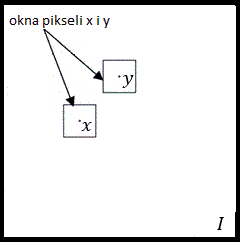
\includegraphics[scale=1]{rysunki/3_fig3.png}
	\caption{Kształt okien wykorzystywanych do obliczania wartości $w(x,y)$.}
	\label{3_fig3}
\end{figure}
gdzie $r$ to zdefiniowana wcześniej stała skalująca wartości podobieństwa pomiędzy pikselami, a operator "$\cdot$" oznacza okna scentrowane względem piksela $x$ oraz $y$ (\autoref{3_fig3}), na podstawie których liczone jest podobieństwo. Normę macierzową występującą w przedstawionej zależności można wyznaczyć korzystając z normy Frobeniusa:
\begin{equation}
{\|I\left(x+\cdot \right)-I\left(y+\cdot \right)\|}_F=\ \sum^{p_s}_{i=1}{\sum^{p_s}_{j=1}{{\left(I(x+\cdot)\big|_{i,j}-I(y+\cdot)\big|_{i,j}\right)}^2}}
\label{FROBENIUS}
,
\end{equation}
gdzie wartość $p_s$ odpowiada wielkości badanego fragmentu obrazu i stanowi wcześniej zdefiniowany parametr. Zmienna $G_\sigma$ reprezentuje macierz o rozmiarze zgodnym z operatorem otoczenia danego piksela "$\cdot$" - $p_s$. Wartości macierzy pozwalają stopniować wpływ każdego z rozpatrywanych pikseli na uzyskiwany wynik poprzez przyznawanie większego priorytetu pikselom centralnym, przy deprecjonowaniu pikseli bardziej oddalonych od centrum. Dla $G_\sigma$ zachodzi zależność:
\begin{align}
\int_{I(x+\cdot)}G_{\sigma}(y)dy = 1.
\end{align}
Rozważając okno Gauss'owskie $G_\sigma$ możemy je opisać zależnością:
\begin{align}
G_\sigma(z)=\frac{1}{Z}\exp\left(-\frac{\|z\|}{2\sigma^2}\right),
\label{oknoGaussowskie}
\end{align}
gdzie $\sigma$ odpowiada odchyleniu standardowemu, a $Z$ współczynnikowi normalizującemu. Podobnie jak w przypadku gradientu nielokalnego funkcja wagi stanowi przekształcenie $D \times D\longrightarrow R$. Kolejnymi ważnymi nielokalnymi operatorami wykonanymi w punkcie $x$ są: 
\begin{itemize}
\item
iloczyn skalarny dwóch nielokalnych przekształceń typu $\overrightarrow{p}:D \times D \longrightarrow R$ (przekształceniem $\overrightarrow{p}$ może być wspomniana funkcja wagi, bądź nielokalny gradient):
\begin{equation}
\left({\overrightarrow{p}}_1\cdot {\overrightarrow{p}}_2\right)(x)\triangleq \int_D{p_1(x,y)\cdot p_2\left(x,y\right)dy}
\label{NLPRODUCT}
,
\end{equation}
\item
moduł przekształcenia $\overrightarrow{p}$:
\begin{equation}
\left|\overrightarrow{p}\right|\left(x\right)\triangleq \sqrt{(\overrightarrow{p}\cdot \overrightarrow{p})}=\sqrt{\int_D{{\big(p(x,y)\big)}^2\mathrm{d}y}}
\label{NLMOD}
,
\end{equation}
\item
dywergencja przekształcenia $\overrightarrow{p}$:
\begin{equation}
({\mathrm{\nabla }}_{NL}\cdot \overrightarrow{p})(x)\ \triangleq \int_D{\big(p\left(x,y\right)-p\left(y,x\right)\big)\sqrt{w(x,y)}\mathrm{d}y}
\label{NLDIV}
,
\end{equation}
\item
laplasjan przekształcenia
\begin{equation}
{\mathrm{\Delta }}_{NL}\overrightarrow{p}(x)\ \triangleq \frac{1}{2}{\mathrm{\nabla }}_{NL}\cdot \Big({\mathrm{\nabla }}_{NL}I\left(x\right)\Big)=\int_D{\Big(I\left(y\right)-I\left(x\right)\Big)w(x,y)\mathrm{d}y}
\label{NLLAP}
.
\end{equation}
\end{itemize}
Warto zauważyć, iż w przypadku przekształceń w postaci gradientu nielokalnego \eqref{NLGRAD} oraz wagi \eqref{NLWEIGHT} zachodzą odpowiednio zależności:
\begin{align}
\Big(p\left(x,y\right)-p\left(y,x\right)\Big) &= \Big({\mathrm{\nabla }}_{NL}I\left(x,y\right)-{\mathrm{\nabla }}_{NL}I\left(y,x\right)\Big)  \notag =\\ 
&= \Big({\mathrm{\nabla }}_{NL}I\left(x,y\right)+{\mathrm{\nabla }}_{NL}I\left(x,y\right)\Big) \notag =\\
&=2{\mathrm{\nabla }}_{NL}I\left(x,y\right) .
\label{NLPOM}
\end{align}
Stąd w szczególnym przypadku dywergencję nielokalną można przedstawić jako: 
\begin{equation}
\Big({\mathrm{\nabla }}_{NL}\cdot \overrightarrow{p}\Big)(x)\ \triangleq \int_D{2\Big(p\left(x,y\right)\Big)\sqrt{w(x,y)}dy}
\label{NLDIVSMART}
,
\end{equation}
\begin{equation}
w(x,y) = w(y,x)
\label{SMARTWEIGHT}
.
\end{equation}
Dywergencja nielokalna stanowi przekształcenie $D \times D \longrightarrow D$.
W celu dyskretyzacji powyższych równań należy zgodnie z \cite{gilboa2008nonlocal} wprowadzić pojęcie okna poszukiwania ${\mathrm{N}}_x$, gdzie $x\in D,\ y\in {\mathrm{N}}_x$. ${\mathrm{N}}_x$ jest podzbiorem obrazu składającym się z punktów będących otoczeniem punktu $x$. Rozmiar okna stanowi wcześniej zdefiniowany parametr. Dla wszystkich pikseli w oknie zachodzi zależność ${\mathrm{N}}_x\coloneqq \left\{y:w_{x,y}>0\right\}$. Wprowadzenie okna skutkuje ograniczeniem wcześniej wprowadzonego przekształcenia $D \times D\longrightarrow R$ do $\mathrm{N} \times D\longrightarrow R$.
\begin{figure}[!h]
	\centering
	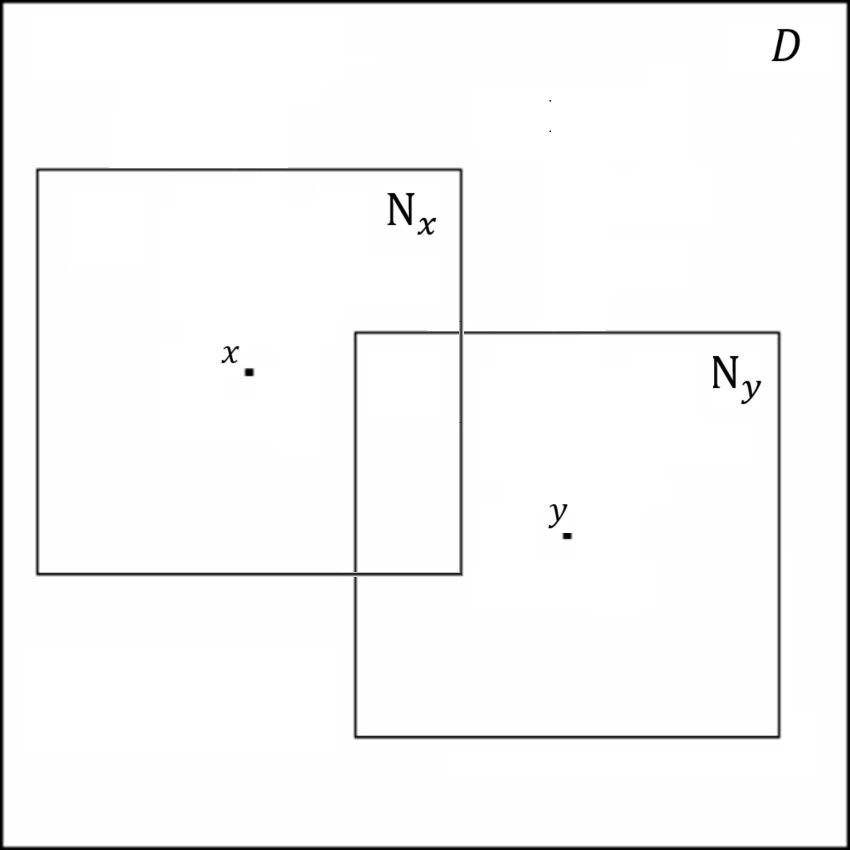
\includegraphics[scale=0.4]{rysunki/3_fig4.png}
	\caption{Przykładowe okna ${\boldsymbol{\mathrm{N}}}_{\boldsymbol{x}}\boldsymbol{,\ }{\boldsymbol{\mathrm{N}}}_{\boldsymbol{y}}$ utworzone dla pikseli $\boldsymbol{x},\boldsymbol{y}$.}
	\label{3_fig4}
\end{figure}
Operatory nielokalne można przedstawić w postaciach dyskretnych:
\begin{large}
\begin{equation}
{\mathrm{\nabla }}_{NLd}I|_{x,y}\triangleq \left(I_y-I_x\right)\sqrt{w_{x,y}}
\label{DNLGRAD}
,
\end{equation}
\begin{equation}
w_{x,y}={\mathrm{exp} \left\{-\sum_{y\in N_x,k\in N_y \\
}{{G_{\sigma}}_y \ast {\left|I_y-I_k\right|}^2}\right\}\ }
\label{DNLWEIGHT}
,
\end{equation}
\begin{equation}
{\left|\overrightarrow{p}\right|}_x\triangleq \sqrt{\sum_{y\in N_x \\ 
}{{\left(p_{x,y}\right)}^2}}
\label{DNLMAG}
,
\end{equation}
\begin{equation}
{\mathrm{\nabla }}_{NLd}\cdot \overrightarrow{p}\big|_x \triangleq \sum_{ 
y\in N_x \\ 
}{\left(p_{x,y}-p_{y,x}\right)}\sqrt{w_{x,y}}
\label{DNLDIV}
,
\end{equation}
\begin{equation}
{\mathrm{\Delta }}_{NL}{\overrightarrow{p}}\big|_x \triangleq \sum_{
y\in N_x \\ 
}{\left(I_y-I_x\right)}w_{x,y}
\label{DNLLAP}
.
\end{equation}
\end{large}
W szczególnym przypadku dla \eqref{NLDIVSMART} można zapisać:
\begin{large}
\begin{equation}
{\mathrm{\nabla }}_{NLd}\cdot \overrightarrow{p}\big|_x \triangleq \sum_{ 
y\in N_x \\ 
}{2p_{x,y}}\sqrt{w_{x,y}}
\label{DNLDIVSMART}
\end{equation}
\end{large}
Warto zauważyć, iż indeksy $x,y$ wskazują na konkretny piksel w obrazie. Lokalizacji w przestrzeni $2D$ dokonuje się przez znajomość par: $x=(i_x,j_x)$ oraz $y=(i_y,j_y)$.
Model nielokalny wariacji całkowitej funkcji oznaczany $NLTV$ (non-local total variation) definiowany dla obrazów w odcieniach szarości przyjmuje następującą postać \cite{rudin1992nonlinear}:
\begin{equation}
{\mathop{\mathrm{min}}_{u} \left\{E\left(u\right)=\ \int_D{\left|{\mathrm{\nabla }}_{NL}u(x)\right|}dx+\frac{1}{2}\int_D{\chi{\left(u-I^0\right)}^2}dx\ \right\}\ }
\label{NLTVGRAY}
,
\end{equation}
gdzie $I^0$ stanowi oryginalny obraz wejściowy, natomiast $u\left(x\right):D\mathrm{\longrightarrow }\mathrm{R}$ obraz wynikowy, będący obrazem wmalowanym, bądź w przypadku pierwotnych założeń obrazem z usuniętym szumem. W przypadku zagadnienia wmalowywania zmienna ${\chi }$ jest funkcją definiowaną na podstawie maski obrazu przyjmująca następujące wartości:
\begin{equation}
\chi \left(x\right)=\Bigg\{ \begin{array}{ll}
0, & \text{dla} \ x \in \Omega \\ 
1, & \text{dla} \ x \in D/ \Omega \end{array}
\label{maskFunction}
.
\end{equation}
Tak zdefiniowany model można przekształcić wykorzystując operację podziału Bregman’a \cite{bresson2009short}. Podział ten stosuje się w celu poprawienia wydajności obliczeniowej w przypadku dyskretnej implementacji problemu minimalizacji energii. Wprowadzenie pomocniczej zmiennej $\overrightarrow{v}=v\left(x,y\right):\ \mathrm{\Omega }\mathrm{\ } \times \ \mathrm{\Omega }\longrightarrow R$ i parametru Bregman’a $\overrightarrow{b}=\overrightarrow{b}\left(x,y\right):\ \mathrm{\Omega }\mathrm{\ }\times \ \mathrm{\Omega }\longrightarrow R$ pozwala przekształcić problem minimalizacji energii opisanej równaniem \eqref{NLTVGRAY} do następującej postaci iteracyjnej \cite{bresson2009short}:
\begin{align}
\begin{aligned}
\left(u^{k+1},{\overrightarrow{v}}^{k+1}\right) &= arg\ \mathop{\mathrm{min}}_{u,\overrightarrow{v}} E\left(u,\overrightarrow{v}\right)=\\ 
&= \biggl\{arg\ \mathop{\mathrm{min}}_{u,\overrightarrow{v}}
\int_D{|\overrightarrow{v}|\left(x\right)}dx+\frac{1}{2}\int_D{{\chi }{\left(u-I^0\right)}^2}dx+\\
&+  \frac{\mathrm{\Theta }}{2}\int_D{{\left|\overrightarrow{v}-{\mathrm{\nabla }}_{NL}u-{\overrightarrow{b}}^{k+1}\right|}^2(x)}dx\ \biggr\},
\end{aligned}
\label{NLTVGRAYMINPROB}
\end{align}
\begin{align}
{\overrightarrow{b}}^{k+1}={\overrightarrow{b}}^k+{\mathrm{\nabla }}_{NL}u^k-{\overrightarrow{v}}^k, {\overrightarrow{b}}^0={\overrightarrow{v}}^0=0.
\label{BREGMANVARIABLE}
\end{align}
gdzie $\Theta$ stanowi wcześniej zdefiniowany parametr algorytmu. Stosując podstawowe równanie rachunku wariacyjnego w postaci równania Eulera-Lagrange’a, metodę przedstawioną w \cite{tai2011fast} oraz schemat iteracyjny Gauss’a-Seidel’a, powyższe równania można sprowadzić do problemu iteracyjnego rozwiązania następujących zależności:
\begin{align}
\chi \left(u-I^0\right)+\mathrm{\Theta }{\mathrm{\nabla }}_{NL}\cdot \left({\overrightarrow{v}}^k-{\mathrm{\nabla }}_{NL}u-{\overrightarrow{b}}^{k+1}\right)=0,
\label{ELNLTV1}
\end{align}
\begin{align}
{\overrightarrow{v}}^{k+1}\mathrm{=}{\mathrm{max} \left(\left|{\mathrm{\nabla }}_{NL}u^{k+1}+{\overrightarrow{v}}^{k+1}\right|-\frac{1}{\mathrm{\Theta }},0\right)\cdot\frac{{\mathrm{\nabla }}_{NL}u^{k+1}+{\overrightarrow{b}}^{k+1}}{\left|{\mathrm{\nabla }}_{NL}u^{k+1}+{\overrightarrow{b}}^{k+1}\right|}\ }.
\label{ELNLTV2}
\end{align}
Zależności te można stosować do obrazów w odcieniach szarości, bądź obrazów kolorowych używając do  każdej z poszczególnych warstw osobnego algorytmu iteracyjnego. Zgodnie z \cite{duan2015fast} takie rozwiązanie prowadzi do niezachowania odpowiedniego kontrastu odrestaurowanej części obrazu i niezachowania krawędzi.
W celu uzależnienia od siebie wszystkich warstw obrazu autorzy w \cite{duan2015fast} proponują zastosowanie funkcjonału $MTV$ przedstawionego w \cite{yang2009fast}, funkcjonału $CTV$ przedstawionego w \cite{blomgren1998color}, bądź modelu Mumford-Shah’a dokładnie opisanego w \cite{jung2011nonlocal}. Ze względu na wydajniejszą implementację oraz najlepsze wyniki uzyskiwane w przypadku modelu \textbf{$CTV$} został on wybrany do badań w niniejszej pracy. Jeśli wykorzystamy wspomniany funkcjonał to zagadnienie minimalizacji energii przyjmie postać:
\begin{align}
{\mathop{\mathrm{min}}_{u} \left\{E\left(u\right)=\sqrt{\sum^m_{i=1}{{\left(\int_D{\left|{\mathrm{\nabla }}_{NL}u(x)\right|}dx\right)}^2}}+\frac{1}{2}\sum^m_{i=1}{\int_D{\chi{\left(u_i-I^0_i\right)}^2}dx}\ \right\}\ },
\label{ENLCTV}
\end{align}
przy czym $m$ odpowiada ilości warstw tworzących obraz kolorowy. Zastosowanie równania rachunku wariacyjnego postaci Eulera-Lagrange’a w swoim rozwiązaniu prowadzi do konieczności obliczenia nielokalnej krzywizny krzywej, będącej w przypadku dyskretyzacji rozwiązania znacząco obciążającą obliczeniowo operacją. W tym celu, podobnie jak w przypadku poprzedniego modelu $NLTV$ zastosowany zostanie heurystyczny algorytm podziału Bregman’a. Analogicznie wprowadzone zostają zmienne $\overrightarrow{v}=\big({\overrightarrow{v}}_1,{\overrightarrow{v}}_2,\ \dots ,\ \ {\overrightarrow{v}}_m\big)$ oraz $\overrightarrow{b}=\left({\overrightarrow{b}}_1,{\overrightarrow{b}}_2,\ \dots ,\ \ {\overrightarrow{b}}_m\right)$. Wtedy przytoczona energia przyjmuje iteracyjną postać:
\begin{align}
\begin{aligned}
\mathop{\mathrm{min}}_{u}E\left(u\right) &= \mathop{\mathrm{min}}_{u}\Biggl\{\sqrt{\sum^m_{i=1}{{\left(\int_D{\left|\overrightarrow{v_i}\right|(x)}dx\right)}^2}}+\\ 
&+\frac{1}{2}\sum^m_{i=1}{\int_D{ \chi {\left(u_i-I^0_i\right)}^2}dx} 
+\frac{\theta }{2}\sum^m_{i=1}{\int_D{{\left|\overrightarrow{v_i}-{\mathrm{\nabla }}_{NL}u_i- {\overrightarrow{b_i}}^{k+1}\right|}^2\left(x\right)}dx}\Biggr\},
\end{aligned}
\label{ENLCTV1}
\end{align}
\begin{align}
{\overrightarrow{b_i}}^{k+1}={\overrightarrow{b_i}}^k+{\mathrm{\nabla }}_{NL}u^k_i-{\overrightarrow{v_i}}^k,\ {{\overrightarrow{b}}_i}^0={\overrightarrow{v_i}}^0=0.
\label{ENLCTV2}
\end{align}
Przyjmując naprzemienną strategię minimalizacji energii można uzyskać równania Eulera-Lagrange’a wyznaczone oddzielnie względem zmiennych $u$ oraz $v$:
\begin{align}
\chi \left(u_i-I^0_i\right)+\mathrm{\Theta }{\mathrm{\nabla }}_{NL}\cdot \left({\overrightarrow{v_i}}^k-{\mathrm{\nabla }}_{NL}u_i-{{\overrightarrow{b}}_i}^{k+1}\right)=0,
\label{ELNLCTV1}
\end{align}
\begin{align}
\mathrm{\Theta }\left(\overrightarrow{v_i}\mathrm{-}{\mathrm{\nabla }}_{NL}u^{k+1}_i\mathrm{-}{{\overrightarrow{b}}_i}^{k+1}\right)\mathrm{+}\frac{\int_D{\left|\overrightarrow{v_i}\right|(x)}dx}{\sqrt{\sum^m_{i=1}{{\left(\int_D{\left|\overrightarrow{v_i}\right|(x)}dx\right)}^2}\ }}\frac{\overrightarrow{v_i}}{\left|\overrightarrow{v_i}\right|(x)}\mathrm{=0}.
\label{ELNLCTV2}
\end{align}
W celu przedstawienia dyskretnej postaci równań \eqref{ELNLCTV1} i \eqref{ELNLCTV2} wygodnym będzie zapis dla konkretnego piksela $z\in D$ w obrazie. W przypadku \eqref{ELNLCTV1} mamy: 
\begin{align}
\chi_z \left[{(u_i)}_z-{\left(I^0_i\right)}_z \right]+\mathrm{\Theta}{\mathrm{\nabla}}_{NL}\cdot \left[ \left({{\overrightarrow{v_i}}^k}\right)_z-{{\mathrm{\nabla}}_{NL}u_i}\big|_z-{\left({{\overrightarrow{b}}_i}^{k+1}\right)}_z \ \right]=0 .
\label{DELNLCTV1}
\end{align}
Korzystając z dyskretnych postaci równań \eqref{NLGRAD}, \eqref{NLWEIGHT}, \eqref{NLPRODUCT} i \eqref{NLDIV} równanie \eqref{ELNLCTV1} można przedstawić w postaci:
\begin{large}
\begin{align}
\begin{aligned}
{u^{k+1}_i}_{z} &= \frac{1}{\chi_z+2\mathrm{\Theta} \sum\limits_{y\in N_i} \left({w_i}\right)_{z,y}} \Biggl[2\mathrm{\Theta }\sum_{y\in N_i} {{{u^k_i}_y \left({w_i}\right)}_{z,y}}+\\
&+ \chi_z \ {I^0_i}_z -\\
&-\mathrm{\Theta} \Biggl[\sum_{y\in N_z} \left({ \left( v^k_i \right)}_{z,y} - { \left( v^k_i \right)}_{z,y} - { \left( v^k_i \right)}_{z,y} + { \left( v^k_i \right)}_{z,y}\right) \sqrt{{\left(w_i\right)}_{z,y}} \Biggr].
\end{aligned}
\label{uNLCTV}
\end{align}
\end{large}
W przypadku równania \eqref{ELNLCTV1} Eulera-Lagrange’a należy przekształcić je względem zmiennej $\overrightarrow{v}$:
\begin{align}
\begin{aligned}
{\overrightarrow{v_i}}^{k+1} &= \mathrm{max} \left(\left|{\mathrm{\nabla }}_{NL}u^{k+1}_i+{\overrightarrow{b_i}}^{k+1}\right|-\frac{\int_D{\left|\overrightarrow{v_i}\right|(x)}dx}{\mathrm{\Theta }\sqrt{\sum^m_{i=1}{{\left(\int_D{\left|{\overrightarrow{v_i}}^k\right|(x)}dx\right)}^2}\ }},0\right) \cdot\\ 
&\cdot \frac{{\mathrm{\nabla }}_{NL}u^{k+1}_i+{{\overrightarrow{b}}_i}^{k+1}}{\left|{\mathrm{\nabla }}_{NL}u^{k+1}_i+{\overrightarrow{b_i}}^{k+1}\right|}.
\label{DELNLCTV2}
\end{aligned}
\end{align}
Podobnie, korzystając z dyskretnych wersji równań \eqref{NLGRAD}, \eqref{NLWEIGHT}, \eqref{FROBENIUS}, \eqref{NLPRODUCT} i \eqref{NLDIV} równanie \eqref{DELNLCTV2} można przedstawić w postaci:
\begin{align}
{{\overrightarrow{v_i}}^{k+1}}_z \cong {\mathrm{max} \left({\left|A^{k+1}_i\right|}_z-\frac{B^k_i}{\mathrm{\Theta }\sqrt{\sum^m_{i=1}{{\left(B^k_i\right)}^2}\ }},0\right)\frac{\left(A^{k+1}_i\right)_z}{{\left|A^{k+1}_i\right|}_z}\ },
\label{VNLCTVITER}
\end{align}
gdzie:
\begin{align}
{A^{k+1}_i}_z=\left({\left(u^{k+1}_i\right)}_y-{\left(u^{k+1}_i\right)}_z\right)\sqrt{{\left(w_{i}\right)}_{z,y}}+{\left(b^{k+1}_i\right)}_{z,y},
\end{align} 
\begin{align}
{\left|A^{k+1}_i\right|}_z=\sqrt{\sum_y{{\left[\left(\left(u^{k+1}_i\right)_y-\left(u^{k+1}_i\right)_z\right)\sqrt{\left(w_i\right)_{z,y}}+\left(b^{k+1}_i\right)_{z,y}\right]}^2}\ },
\end{align}
\begin{align}
B^k_i=\sum_z{\sqrt{\sum_y{\left({v^k_i}^2\right)_{z,y}}}}.
\end{align}
\textbf{Warto przypomnieć, iż w przytoczonych wzorach $y$ odpowiada pikselom znajdującym się oknie poszukiwania ${\mathrm{N}}_z$ scentrowanym względem piksela $z$, natomiast $i$ odpowiada $i$-tej warstwie spośród warstw tworzących obraz kolorowy}. Autorzy w \cite{jung2011nonlocal} proponują zmodyfikowany sposób wyznaczania wagi uwzględniający kształt maski w obrazie:
\begin{align}
w\left(x,y\right)\triangleq {\mathrm{exp} \left\{-\frac{G_{\sigma }*{\chi }_R\left(x+\ \cdot \right){\left|I\left(x+\ \cdot \right)-I\left(y+\ \cdot \right)\right|}^2}{r^2}\right\}\ },
\label{NLWEIGHTMASK}
\end{align}
gdzie:
\begin{equation}
{\chi }\left(x\right)=\Bigg\{ \begin{array}{ll}
0, & \text{dla} \ x \in  \mathrm{\Omega} \\ 
1, & \text{dla} \ x \in  D/\mathrm{\Omega} \end{array}
.
\end{equation}
Podsumowując algorytm wmalowywania w oparciu o model $NLCTV$ z algorytmem podziału Bregman’a można przedstawić w następujących krokach:
\begin{enumerate}[I.]
\item  
Inicjalizacja zmiennych $k=0,\ \overrightarrow{b^0_i}=0,\ \overrightarrow{v^0_i}=0,\ u^0_i=f^0_i$.
\item  
Wyznaczenie wagi $w_i$ zgodnie z równaniem \eqref{NLWEIGHTMASK} dla całego obszaru obrazu $D$.
\item  
Powtarzanie aż do wyznaczenia całego nieznanego obszaru $\Omega$:
\begin{enumerate}[1)]
\item
wyznaczenie wartości $u_x$ dla każdego piksela $x$, dla którego $p_x$ zawiera conajmniej jeden punkt z poza obszaru $\Omega$, $k$ oznacza krok iteracji procesu minimalizacji w celu wyznaczenia $u$:
\begin{enumerate}[a)]
\item
\noindent wyznaczenie ${\overrightarrow{b}}^{k+1}={\overrightarrow{b}}^k+{\mathrm{\nabla }}_{NL}u^k-{\overrightarrow{v}}^k$,
\item
\noindent wyznaczenie $u^{k+1}$ na podstawie \eqref{DELNLCTV1},
\item
\noindent wyznaczenie $v^{k+1}$ na podstawie \eqref{VNLCTVITER}.
\end{enumerate}
\item  
Aktualizacja wagi $w_i$ w wypełnionym obszarze, pomniejszenie obszaru $\mathrm{\Omega }$ o wypełnione piksele.
\end{enumerate}
\end{enumerate}
\subsection{Uproszczona wersja rozwiązania.}
Złożoność obliczeniowa algorytmu $NLCTV$ powoduje, że czas potrzebny na obliczanie nowych wartości w obrazie wydłuża się. W celu skrócenia tego czasu Autorzy artykułu \cite{ColorTextureInpaintingNLCTVModel} udostępniają rozwiązanie oparte na następującej aproksymacji równania \eqref{uNLCTV}, pozwalającej uzyskać wyniki zbliżone do wyników oryginalnego algorytmu:
\begin{align}
\begin{aligned}
{{\left(u_i\right)}_l}^{k+1} &= \frac{1}{{\left({\lambda }_D\right)}_l+2\mathrm{\Theta} \sum\limits_{j\in N_i} {\left(w_i\right)}_{l,j}\ } \Biggl[2\mathrm{\Theta }\sum_{j\in N_i} {{{\left(u^k_i\right)}_j\left(w_i\right)}_{l,j}\ }\\
&+ {\left({\lambda }_D\right)}_l{\left(f_i\right)}_l\Biggr].
\end{aligned}
\label{NLH1}
\end{align}
W przytoczonym równaniu eliminacja zmiennych $v$ oraz $b$ pozwala znacznie ograniczyć wykorzystywane zasoby pamięciowe i przyspieszyć działanie algorytmu dzięki pominięciu dodatkowych obliczeń wykluczonych zmiennych. Korzyści czasowe oraz różnice w obliczonych obrazach opisany zostanie w podrozdziale \ref{ssec:NLCTVModSec}.
\section{Wariacyjny model nielokalny wmalowywania - VFI}
\label{sec:sVFI}
Kolejną z rozważanych metod będzie metoda zaproponowana przez Fedorov'a, Facciolo i Arias'a w \cite{arias2011variational}. Autorzy tej publikacji proponują optymalizację energii $\mathcal{E}(\varphi(x), u(\Omega))$ zależnej:
\begin{itemize}
\item
od nieznanego obszaru obrazu $u(\Omega)$,
\item
od mapy podobieństwa będącej funkcją przypisującą każdemu punktowi z nieznanego obszaru jego konkretny odpowiednik z obszaru znajdującego się poza maską $\varphi(x)$.
\end{itemize}
\begin{figure}[!h]
	\centering
	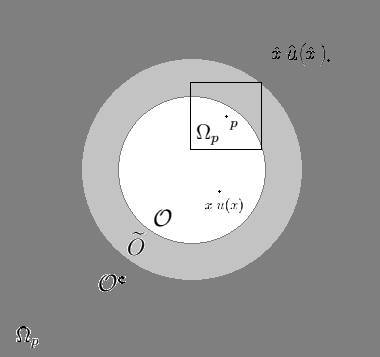
\includegraphics[scale=0.6]{rysunki/6_fig1}
	\caption{Określenie charakterystycznych obszarów obrazu. Rysunek autorski.}
	\label{6_fig1}
\end{figure}
Niech $u(x)$ oznacza funkcję przekształcającą zbiór $\Omega$ według zależności  $u:\Omega \rightarrow R$, gdzie $\Omega$ to obszar do uzupełnienia.
Niech $\hat{u}(\hat{x})$ oznacza funkcję przekształcającą zbiór $D$ według zależności $\hat{u} : D \rightarrow R$, gdzie $D$ to obszar oryginalnego obrazu nie podlegający modyfikacji.
Ponad to niech $\mathrm{N}_x$ i $\mathrm{N}_{\hat{x}}$ oznaczają podzbiory punktów obrazu scentrowane odpowiednio względem punktów $x$ i $\hat{x}$.
Wtedy zbiór $\widetilde{\Omega}$ definiuje się jako $\widetilde{\Omega} := \Omega + \sum {\mathrm{N}}_x$, gdzie $\sum {\mathrm{N}}_x$ to suma wszystkich podzbiorów utworzonych względem punktów $x \in \Omega$. Ostatecznie $D^c = D / \widetilde{\Omega}$.
Zgodnie z \cite{arias2011variational} przekształcenie $u(x)$ jest zarezerwowane dla obszaru maski (obszaru wmalowywanego), a $\hat{u}(\hat{x})$ odpowiada przekształceniu w niezmienianym obszarze obrazu $D$). 
Przekształcenie funkcji podobieństwa $\varphi(x)$ przedstawia \autoref{6_fig2}.
\begin{figure}[!h]
	\centering
	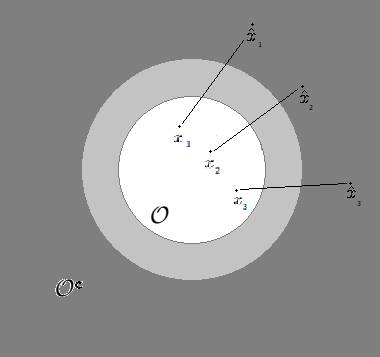
\includegraphics[scale=0.7]{rysunki/6_fig2}
	\caption{Funkcja podobieństwa $\varphi(x)$ : $\varphi(x_1)=\hat{x_1}, \varphi(x_2)=\hat{x_2}, \varphi(x_3)=\hat{x_3}$. Rysunek autorski.}
	\label{6_fig2}
\end{figure}
Energię poddawaną minimalizacji można wyrazić zależnością:
\begin{align}
\begin{aligned}
\mathcal{E}(u,\varphi) = \int_{\mathcal{\widetilde{O}}}\int_{\Omega_p}\abs{u(x+h) - \hat{u}(\varphi(x)+h)}^2\mathrm{dhdx}.
\end{aligned}
\end{align}
Funkcja ta jest niewypukła, stąd proces minimalizacji pozwala odnaleźć jedynie lokalne minima. W pracy wykorzystano iteracyjny algorytm naprzemiennej minimalizacji polegający na wyznaczaniu w każdym kroku $u(x)$ względem ustalonej wartości $\varphi(x)$, a następnie $\varphi(x)$ względem ustalonej wartości $u(x)$.
\subsection{Wyznaczenie mapy podobieństwa.}
\label{ssec:wyznaczanieMapySection}
W przypadku gdy przyjmiemy ustaloną wartość $u(x)$ (czyli $u(x) = $ const), to proces minimalizacji można opisać zależnością:
\begin{align}
\begin{aligned}
\mathop{\operatorname{arg \ min}}_{t} \ \mathcal{E}\biggl( u(x+\cdot) - {\hat{u}}\bigl((x+t)+\cdot\bigr)\biggr),\operatorname{gdzie} \ \forall \ t : x+t \in D^c
\label{minNNF}
\end{aligned}
.
\end{align}
Przez symbol $(x+\cdot)$ rozumiemy podmacierz punktów otaczających punkt $x$. 
Zmienna $t$ w tym zagadnieniu przyjmuje takie wartości ze zbioru wektorów przemieszczeń, których suma z danym wektorem położenia $x$ lokalizuje go w obszarze $D^c$ (podobnie jak na \autoref{6_fig2}, $ \ \hat{x} = x + t$, $ \ x = \hat{x} - t$). Wynikiem minimalizacji jest $\varphi$, która stanowi funkcję wyznaczającą najbliższego sąsiada punktu $x$ z przestrzeni $D^c$, $\varphi :\Omega \rightarrow D^c$. Warto zaznaczyć, że przez pojęcie najbliższego sąsiada punktu $x$ rozumiemy nie punkt znajdujący się najbliżej, ale ten piksel, dla którego zgodnie z przyjętą normą uzyskuje się najniższą wartość z pośród wszystkich możliwych:
\begin{align}
\begin{aligned}
\big\| u(x + \cdot) - \hat{u}(\hat{x}+\cdot) \big\| 
\label{normNNF}
\end{aligned}
.
\end{align}
Propozycje definicji normy są przedstawione przez autorów w \cite{MathematicalModelsforNLTextureInpainting} i zostaną opisane w dalszej części tej pracy magisterskiej. Warto zauważyć, że normę tę można również zdefiniować za pomocą równań \eqref{NLWEIGHT} bądź \eqref{FROBENIUS}. Najprostszy algorytm wyznaczania najbliższego sąsiada może osiągnąć złożoność do $O(N^3)$ i może on wymagać znacznych nakładów obliczeniowych. Autorzy w \cite{arias2011variational} proponują zastosowanie algorytmu \textbf{PatchMatch} dokładnie opisanego w \cite{barnes2009patchmatch}. Algorytm ten oparty jest na dwóch krokach. Niech punkt $x$ odpowiada współrzędnym $i, j$ obrazu, natomiast dla uproszczenia zapisu oznaczmy $u(x+\cdot)$ jako $p_u(i,j)$. Wtedy kroki te można opisać następująco:
\begin{enumerate}
\item
Losowo inicjalizujemy piksele.
\item
Definiujemy skończoną liczbę iteracji i wykonujemy następujące czynności:
\begin{enumerate}[a)]
\item
propagacja: w przypadku iteracji o numerze parzystym dla sprawdzenia wszystkich pikseli $x$ z maski w kierunku rastrowym przedstawionym na \autoref{6_fig3}, czy 
wartość $\big\| p_u(i,j) - p_{\hat{u}}\big(\varphi(i+1,j)\big) \big\|$, bądź $\big\| p_{u}(i,j) - p_{\hat{u}}\big(\varphi(i,j+1)\big) \big\|$ nie jest mniejsza od obecnie wyznaczonej wartości i w takim przypadku należy zmienić najbliższego sąsiada według formuły $\varphi(i,j) = \varphi(i+1,j)$, lub $\varphi(i,j) = \varphi(i,j+1)$, 
w przypadku iteracji o numerze nieparzystym należy sprawdzić dla wszystkich pikseli $x$ w kierunku odwrotnym do kierunku rastrowego przedstawionym na \autoref{6_fig3}, czy 
wartość $\big\| p_{u}(i,j) - p_{\hat{u}}\big(\varphi(i-1,j)\big) \big\|$ bądź $\big\| p_{u}(i,j) - p_{\hat{u}}\big(\varphi(i,j-1)\big) \big\|$ nie jest mniejsza od obecnie wyznaczonej wartości i w takim przypadku trzeba zmienić najbliższego sąsiada według formuły $\varphi(i,j) = \varphi(i-1,j)$, lub $\varphi(i,j) = \varphi(i,j-1)$,
\item
poszukiwanie w oknach: dla każdego punktu $(i,j)$ sprawdzane jest, czy w stopniowo pomniejszanych oknach centrowanych względem punktu $(i,j)$ istnieje losowy punkt $(i', j')$, dla którego zachodzi nierówność $\big\| p_{u}(i,j) - p_{\hat{u}}(i',j') \big\| < \big\| p_{u}(i,j) - p_{\hat{u}}\big(\varphi(i,j) \big)\big\|$, jeśli tak to punkt ten jest podmieniany.
\end{enumerate}
\end{enumerate}
\begin{figure}[!h]
	\centering
	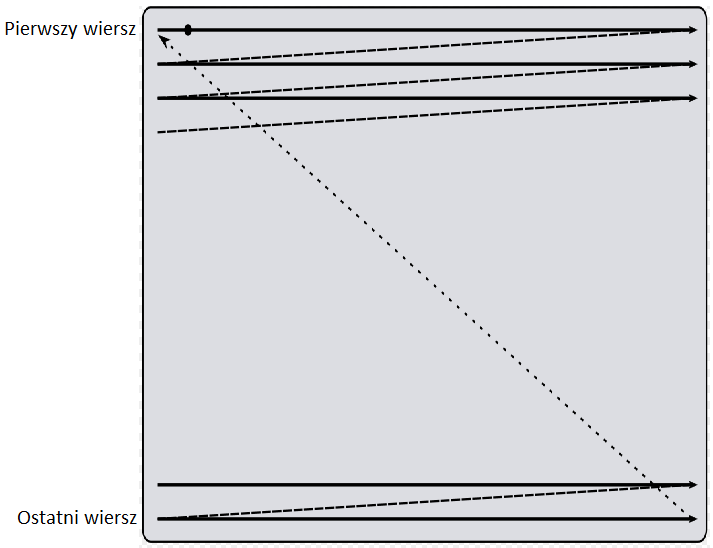
\includegraphics[scale=0.5]{rysunki/6_fig3}
	\caption{Funkcja podobieństwa $\varphi(\hat{x})$ : $x_1 = \varphi(\hat{x_1}), x_2 = \varphi(\hat{x_2}), x_3 = \varphi(\hat{x_3})$.}
	\label{6_fig3}
\end{figure}
Kroki algorytmu \textbf{PatchMatch} zostały przedstawione graficznie na \autoref{6_fig4}.
\begin{figure}[!h]
	\centering
	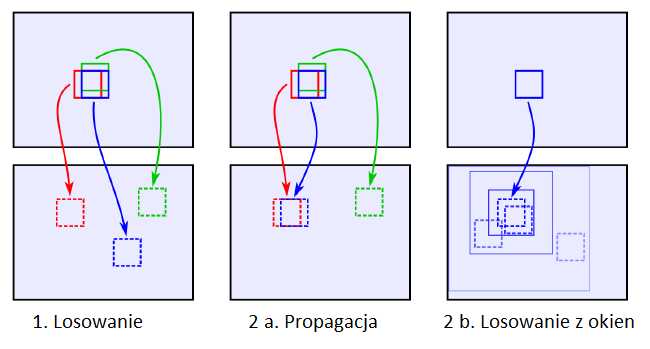
\includegraphics[scale=0.9]{rysunki/6_fig4}
	\caption{Algorytm PatchMatch. Źródło \cite{arias2011variational}.}
	\label{6_fig4}
\end{figure}
\subsection{Wyznaczenie wartości obrazu.}
Niech funkcja $e$  będzie przekształceniem $e: \mathrm{N}_x \rightarrow {\rm I\!R}^{+}$ której wartość reprezentuje sumę ważonych błędów pomiędzy dwoma fragmentami obrazu scentrowanymi względem punktów $x$ i $\hat{x}$. Korzystając z wcześniej wprowadzonych oznaczeń mamy:
\begin{align}
\begin{aligned}
e(x, \hat{x}) &= G_\sigma \ast \big\| u(x + \cdot) - u(\hat{x} + \cdot) \big\| = G_\sigma \ast \big\| p_{u}(x) - p_{\hat{u}}(\hat{x}) \big\| = \\ 
&= \int_{\mathrm{N}_x} G_\sigma(h) \big\| u(x+h) - \hat{u}(\hat{x} +h) \big\|\mathrm{dh},
\label{minUs}
\end{aligned}
\end{align}
gdzie zmienna $G_{\sigma}$ została wprowadzona dla algorytmu $NLCTV$ i opisywana jest zależnością \eqref{oknoGaussowskie}. Autorzy artykułu \cite{arias2011variational} proponują tam minimalizację następującej energii będącej akumulacją błędów pikseli:
\begin{align}
\begin{aligned}
E(u) &= \int_{\widetilde D}\int_{\mathrm{N}_x}G_\sigma(h)\cdot e \left[ u(x+h) - \hat{u}(\varphi(x)+h\right]\mathrm{dhdx}.
\label{patchMatchEnergy}
\end{aligned}
\end{align} 
Niech $z := x+h$ i $\hat{z} := \hat{x}+h$. Wprowadzamy zależność:
\begin{align}
m(z,\hat{z}) = \int_{\mathrm{N}_x}G_\sigma(h)\chi_{z-h}C_{\varphi(z-h)}(\hat{z}-h)\mathrm{dh},
\end{align}
gdzie:
\begin{itemize}
\item
zmienna $\chi$ została już zdefiniowana w modelu $NLCTV$ \eqref{maskFunction} i przyjmuje wartość $1$ poza maską i wartość $0$ w masce,
\item
zmienna $C(p)$ określa pewność - prawdopodobieństwo tego, że nowa wartość wyznaczonego piksela $p \in \Omega$ przyjęłaby właśnie tę wyznaczoną wartość - i jest ona określona następującą zależnością:
\begin{align}
C(x)=(1-c_0)exp\bigg(\frac{-\mathrm{d}\bigl(x,\partial\Omega\bigr)}{t_c}\bigg) + c_0,
\label{pewnoscVFI}
\end{align}
\end{itemize}
przy czym wartość $t_c$ określa szybkość opadania funkcji wykładniczej, $c_0$ asymptotę, do której to funkcja zmierza, a wewnętrzna zależność $\frac{-\mathrm{d}(x,\partial\Omega)}{t_c}$ określa odległość punktu od granicy maski. $C(p)$ dla $p \in D^c$ przyjmuje wartość $1$, natomiast dla $p \in \Omega$ wartość ze zbioru $\langle c_0,1)$ W zależności od zastosowanej normy \eqref{normNNF} rozwiązanie problemu minimalizacji energii uzyskuje różne postacie. Autorzy w \cite{arias2011variational} przedstawiają rozwiązanie dla następujących definicji norm:
\begin{enumerate}
\item
Ważonej nielokalnej normy uśredniającej:
\begin{align}
\begin{aligned}
\big\| p_{u}(x) - p_{\hat{u}}(\hat{x}) \big\|^{2}_{g,2} = g \ast | u(x+\cdot) - \hat{u}(\hat{x}+\cdot) |^2,
\label{nonLocalMeans}
\end{aligned}
\end{align}
\item
Ważonej nielokalnej normy euklidesowej:
\begin{align}
\begin{aligned}
\big\| p_{u}(x) - p_{\hat{u}}(\hat{x}) \big\|_{g,1} = g \ast | u(x+\cdot) - \hat{u}(\hat{x}+\cdot)|,
\label{nonLocalMedians}
\end{aligned}
\end{align}
\item
Nielokalnej normy Poissona:
\begin{align}
\begin{aligned}
\big\| p_{u}(x) - p_{\hat{u}}(\hat{x}) \big\|_{P} &= \big\| p_{u}(x) - p_{\hat{u}}(\hat{x}) \big\|^{2}_{g,2} + \big\| p_{u}(x) - p_{\hat{u}}(\hat{x}) \big\|^{2}_{g,2,\nabla} \\
&= g \ast \Big[\lambda \cdot | u(x+\cdot) - \hat{u}(\hat{x}+\cdot) | + \\
&+ (1-\lambda)\cdot |\nabla u(x+\cdot) - \nabla \hat{u}(\hat{x}+\cdot)|\Big].
\label{nonLocalpoisson}
\end{aligned}
\end{align}
\end{enumerate}
Indeksy dolne $g, 1, 2, \nabla$ przy zapisach nielokalnych norm oznaczają odpowiednio: uwzględnienie zmiennej \eqref{oknoGaussowskie} w wyznaczaniu odległości, normę wektorową $\ell_{1}$, normę wektorową $\ell_{2}$, obliczanie dystansu na podstawie dywergencji rozważanego pola. Stąd suma różnic pikseli w przypadku normy Poissona wymaga dodatkowo wyznaczenia dywergencji obrazu. Współczynnik $\lambda$ określa w jakim stopniu poszczególny człon będzie miał wpływ na ostatecznie uzyskiwany wynik. Dla trzech wspomnianych norm uzyskuje się trzy różne rozwiązania dokładnie przedstawione w pracy \cite{arias2011variational}.
\subsection{Wielostopniowy schemat wypełniania.}
W wielu metodach wypełniania braków w obrazie stosowany jest algorytm wielostopniowy, przykładem mogą być metody opisane w \cite{kawai2009image}, \cite{komodakis2007image} bądź \cite{wexler2007space}. Algorytm ten polega na utworzeniu serii mniejszych przeskalowanych obrazów, następnie wypełnianiu ich począwszy od najmniejszego z warunkami początkowymi uzyskanymi poprzez przeskalowanie do większego obrazu wcześniej wyznaczonych wartości w masce. W przypadku najmniejszego obrazu z serii warunkami początkowymi mogą być:
\begin{itemize}
\item
losowo wyznaczone wartości obrazu pobierane z obszaru $D^c$,
\item
rozwiązanie równania Poisson'a \eqref{Poisson2D}, dokładnie przedstawione w \autoref{chap:navierstokes}, metodą SOR ( z ang. succesive over relaxation method) zgodnie z zależnością \eqref{DiscreteSOR}.
\end{itemize}
Przeskalowywanie w obie strony musi odbywać się w sposób nie zniekształcający głównych struktur, obiektów i tekstur obrazu. W tym celu autorzy \cite{arias2011variational} proponują model piramidy Gauss'a. W celach wmalowywania tworzone są dwie oddzielne piramidy wyznaczające maski obrazu i same obrazy. Niech $S$ oznacza liczbę poziomów piramidy, a rozmiar oryginalnego obrazu jest oznaczany przez $s=0$. Niech rozmiar najmniejszego stopnia określa $A_{S-1}$, natomiast rozmiar oryginalnego obrazu $A_{0}$. Wtedy współczynnik próbkowania wykorzystywany do tworzenia coraz mniejszych obrazów wynosi:
\begin{align}
r := \left(\frac{A_0}{A_{s-1}}\right)^\frac{1}{s-1}.
\end{align}
W rezultacie aby uzyskać mniejszy obraz musi zachodzić zależność $r \geq 1$. Parametr $\sigma$ tworzonego filtru Gauss'a wyznaczany jest z zależności $\sigma(r)=0.62\sqrt{r^2-1}$. Rozmiar okna Gauss'a wykorzystywanego do filtrowania można przyjąć jako wartość stałą zdefiniowaną z góry. Niech indeks górny s odnosi się do zmiennych oraz do obszarów w zakresie rozważanego poziomu piramidy. Opiszmy maskę obrazu \eqref{maskFunction} na stopniu $s$ funkcją $\chi_{\Omega^{s}}$. Wtedy kolejny stopień piramidy $s+1$ dla maski  wyznaczamy z zależności:
\begin{align}
\chi_{\Omega^{s+1}}=(\downarrow_r G_{\sigma(r)} \ast \chi_{\Omega^s}) > T_{0},
\end{align}
gdzie $\downarrow_r$ oznacza, że grupa pikseli w otoczeniu o boku (współczynniku próbkowania) $r$ zostanie zastąpiona jednym pikselem. Zasadą pomniejszania obrazu jest nierówność, dzięki której stosunek pól obszarów $\frac{\Omega}{D}$ na każdym kolejnym stopniu $s$ niewiele się zmniejsza. Autorzy w \cite{arias2011variational} proponują wartość parametru $T_0=0.4$. Wprowadźmy pomocniczą funkcję skalarną $f(x) = \downarrow_r G_{\sigma(r)}\ast\chi_{\Omega^s}(x + \cdot)$. Wtedy ograniczenie możemy prosto wytłumaczyć - w przypadku gdy $f(x)$ będzie większa od $0.4$ to punkt $x$ potraktujemy jako punkt źródłowy obrazu, nie wymagający wmalowania, czyli $x \in D^{s+1}$, w przeciwnym wypadku zachodzi $x \in \Omega^{s+1}.$ W przypadku wyznaczenia obrazu na kolejnym stopniu $s+1$ piramidy wykorzystywana jest zależność:
\begin{align}
u^{s+1}(x)= \downarrow_r \frac{G \ast \chi_{\Omega^s} u^s(x)}{G \ast \chi_{\Omega^s}(x)}
\end{align}
W tej zależności pewnym ograniczeniem próbkowania w dół jest nieuwzględnianie wartości znajdujących się w obszarze $\Omega^s$. Obraz w pierwszym kroku zostaje przemnożony przez maskę przedstawiającą źródłową część obrazu, a następnie poddany operacji splotu z utworzonym filtrem Gauss'a. Mianownik tego równania służy normalizacji obliczenia. Wielostopniowy schemat wypełniania w zastosowaniu do algorytmu $VFI$ opisany w poprzednim rozdziale wymusza przy każdym przejściu ze stopnia $s$ do $s-1$ piramidy oprócz przeskalowania obrazu $u$ przeskalowanie także funkcji mapy podobieństwa $\varphi$. Obraz i mapa stanowią na każdym kolejnym poziomie $s-1$ piramidy aż do ostatniego $S$ warunki początkowe kolejnych kroków naprzemiennej minimalizacji. Do przeskalowania  został wykorzystany algorytm dokładnie przedstawiony w \cite{wexler2007space} i opisany w \cite{arias2011variational}.
\subsection{Podsumowanie algorytmu}
\label{ssec:VFIPodsumowanie}
Jeśli połączymy opisane wcześniej operacje dokonywane na obrazie to algorytm wypełniania brakującego obszaru możemy przedstawić w następujących krokach:
\begin{enumerate}
\item
Ustawienie argumentów algorytmu: obraz $u^{0}$, maska obrazu $\chi$, liczba poziomów piramidy $S$, rozmiar najmniejszego obrazu $A_{S-1}$, ilość iteracji minimalizacji energii $K$.
\item
Wyznaczenie piramidy maski stanowiącej zbiór $\{\chi^s\}_{s=0,...,S-1} \ $, wyznaczenie piramidy obrazu stanowiącej zbiór $\{u^s\}_{s=0,...,S-1} \ $.
\item
Inicjalizacja obrazu $u^{S-1}$ w obszarze $\Omega$ losowymi wartościami, bądź np. rozwiązaniem równania \eqref{DiscreteSOR}. Obliczenie mapy podobieństwa $\varphi^{S-1}$ na podstawie $u^{S-1}$ według opisu zawartego w podrozdziale \ref{ssec:wyznaczanieMapySection}.
\item
Wykonanie dla każdego z poziomów piramidy $s$ począwszy od $S-2$ do $0$ następujących kroków:
\begin{enumerate}[a)]
\item
przeskalowanie mapy podobieństwa $\varphi^s=r \cdot (\uparrow_r \varphi^{s+1})$, gdzie $\uparrow_r$ oznacza, że jedna komórka zostanie zastąpiona podmacierzą o rozmiarze (współczynniku próbkowania) $r$, następnie dla każdej komórki z podmacierzy interpolowanie jej wartości czyli najbliższego sąsiada,
\item
wyznaczenie przeskalowanego obrazu $u^s_0=r \cdot (\uparrow_r u^{s+1})$ i przepisanie wartości $u^s(\Omega)=u^s_0(\Omega)$ w celu inicjalizacji.
\item
przeprowadzenie naprzemiennie założoną z góry ilość razy z wykorzystaniem odpowiedniej normy \eqref{normNNF} dwóch minimalizacji ($i$ oznacza $i$-tą iterację):
\begin{itemize}
\item
\eqref{minNNF} w celu wyznaczenia mapy podobieństwa ${\left(\varphi^s\right)}^i$,
\item
\eqref{minUs} w celu wyznaczenia wartości obrazu ${\left(u^s\right)}^i$ w nieznanym obszarze.
\end{itemize}
\end{enumerate}
\end{enumerate}
Wynikiem powyższego algorytmu jest zbiór obrazów $\{u^s\}$ oraz map podobieństwa $\{\varphi^s\}$, gdzie $s \in {0,...,S-1}$.
\chapter{Uzupełnianie kawałkami obrazu.}
\section{Metoda Criminisi.}
\label{sec:crimMetod}
Kolejną grupą algorytmów rozważanych w niniejszej pracy jest grupa opierająca się na wypełnianiu brakujących obszarów w obrazie fragmentami pochodzącymi z ich otoczenia. W odróżnieniu od wielu algorytmów opierających się na równaniach różniczkowych metoda ta nie wykorzystuje metody dyfuzji. Pierwszy raz zaproponowana została ona w \cite{efros1999texture}, a jej podstawowy krok opiera się na schemacie przedstawionym na \autoref{4_fig1}.
\begin{figure}[!h]
	\centering
	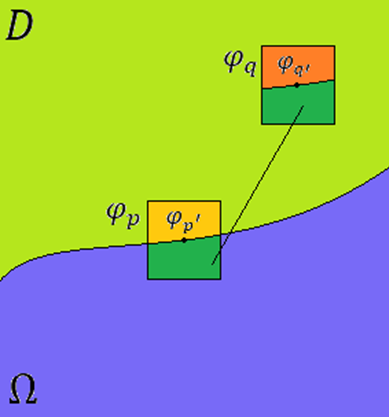
\includegraphics[scale=0.6]{rysunki/4_fig1}
	\caption{Schemat wmalowywania obrazu. Rysunek autorski.}
	\label{4_fig1}
\end{figure}
Podobnie jak w poprzednich rozdziałach zbiór $D$ oznaczony kolorem zielonym
określa znane punkty obrazu, natomiast $\Omega$ oznaczony kolorem fioletowym określa obszar przeznaczony do odrestaurowania.
Oznaczenie $u(\hat{x})$ oznacza funkcję na obszarze $D^c$, $\hat{x}  \in D^c$ (\autoref{6_fig1}).
Niech $q_{\hat{x}}$ stanowi podzbiór wartości punktów obrazu scentrowanych względem piksela $\hat{x}$ o zdefiniowanym z góry promieniu otoczenia.
Dla $q_{\hat{x}}$ zachodzi $\forall p \in q_{\hat{x}} : \chi(p) \neq 0$, gdzie $\chi$ odpowiada funkcji maski opisanej przez formułę \eqref{maskFunction} 
Niech $p_{x}$ stanowi podzbiór punktów tworzących fragment obrazu o rozmiarze równym rozmiarowi $q_{\hat{x}}$, scentrowanych względem piksela $x$, gdzie $x \in \partial \Omega$.
Zdefiniujmy dwa podzbiory punktów:
\begin{align}
\begin{aligned}
p_{x} = s_x + i_x,
\end{aligned}
\end{align}
gdzie $\forall p \in s_x : \chi(p) = 1$ przy czym $s_x$ oznacza wypełnioną część fragmentu oraz $\forall p \in i : \chi(p) = 0$ czyli $i_x$ jako brakująca część fragmentu obrazu.  
Oznaczmy odpowiednio zbiory $\hat{s}_{\hat{x}}$ i $\hat{i}_{\hat{x}}$ będące przesunięciem zbiorów $s_x$ i $i_x$ o wektor $\overrightarrow{|x \hat{x}|}$:
\begin{align}
\begin{aligned}
q_{\hat{x}} = \hat{s}_{\hat{x}} + \hat{i}_{\hat{x}}.
\end{aligned}
\end{align}
Podstawową operacją wmalowywania metodą propagacji tekstury obrazu jest znalezienie pary
 najbardziej podobnych do siebie fragmentów $\left\langle p_{x}, q_{\hat{x}} \right\rangle $ oraz zgodnie z \autoref{4_fig1} przepisanie wartości odpowiednich pikseli z wyznaczonego zbioru $\hat{i}_{\hat{x}}$ do odpowiadających im pikseli w zbiorze $i_x$ oznaczonych kolorem ciemnoniebieskim. Zapisując to w sposób formalny szukamy:
\begin{align}
\mathrm{arg} \mathop{\mathrm{min}}_{\hat{y} \in D^c} \big\| u(p_x) - \hat{u} (q_{\hat{y}} ) \big\| .
\label{FROBDIST}
\end{align}
Autorzy w \cite{criminisi2004region} proponują mierzyć odległość pomiędzy dwoma fragmentami $d\left( u(p_x), \hat{u} (q_{\hat{y}}) \right)$ jako sumę kwadratów różnic odpowiadających sobie pikseli ze zbiorów $s_x$ i ${\hat{s}}_{\hat{y}}$:
\begin{align}
d\left( u(s_x) - \hat{u}( \hat{s}_{\hat{y}} )\right)= \sum_{z \in s_x} \left( \hat{u}(z + \overrightarrow{|x \hat{x}|}) - u(z) \right)^2 .
\label{FROBENIUS2} 
\end{align}
W celu odrestaurowania obrazu powyższy schemat powtarzany jest aż do momentu wypełnienia całego obszaru $\mathrm{\Omega }$.
Metoda wmalowywania pierwszy raz przedstawiona w  \cite{efros1999texture} nie zakłada żadnego priorytetu ani kolejności wypełniania braków ustalanej na podstawie otoczenia maski. Tak przeprowadzana synteza obrazu pomimo wyznaczenia dla danego piksela trafnego dopasowania względem zdefiniowanej odległości może prowadzić do niespójności obrazu, przykład na \autoref{5_fig2}
\begin{figure}[!h]
	\centering
	\includegraphics[scale=0.3]{rysunki/5_fig2}
	\caption{Niespójność obrazu przy najlepszym dopasowaniu. $A$ - odrestaurowywany obraz, $B$ - wynik algorytmu, $C$ - oczekiwany wynik. Rysunek autorski.}
	\label{5_fig2} 
\end{figure}
\begin{figure}[!h]
	\centering
	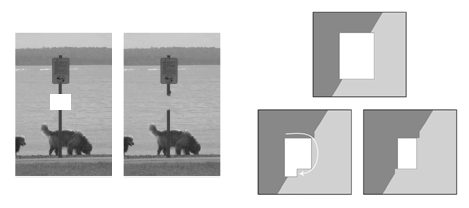
\includegraphics[scale=1]{rysunki/4_fig2}
	\caption{Wpływ prostego schematu wypełniania braków na wynikową teksturę obrazu. Źródło \cite{criminisi2004region}.}
	\label{4_fig2} 
\end{figure}
W 2004 roku Criminisi w \cite{criminisi2004region} skorzystał z koncepcji próbkowania fragmentów obrazu proponując nowe podejście do wyznaczania kolejności ich wmalowywania.  Kolejność wypełniania wyznaczana jest na podstawie izolinii poziomu jasności obrazu. W każdej iteracji algorytmu dla pikseli sąsiadujących z maską wyznaczane są wartości priorytetu wypełniania. Następnie wypełnienie odbywa się dla piksela o największym priorytecie. Dzięki nowemu podejściu izolinie będące granicami struktur obrazu są kontynuowane w miejscach odrestaurowywanych.
Algorytm przedstawiony w \cite{criminisi2004region} opiera się na powtarzaniu trzech głównych kroków w każdej iteracji wykonywanej do momentu wypełnienia wszystkich pikseli ze zbioru $\mathrm{\Omega }$.
Każda kolejna iteracja prowadzi do przesunięcia granicy maski $\partial \Omega$ w jej głąb. Pierwsze dwa kroki w pojedynczej iteracji służą do wyznaczenia priorytetu $P\left(x\right)$ dla każdego piksela obrazu znajdującego się na granicy maski $x \in \partial \Omega$, natomiast trzeci krok służy znalezieniu najlepszego punktu dopasowania $\hat{x}$.
Priorytet $P \left( x \right)$ każdego piksela $x$ wyznaczany jest z zależności:
\begin{align}
P\left( x \right)=C_t(x)\cdot D_t(x).
\label{PRIORITY}
\end{align}
Pierwszy krok w każdej wykonywanej iteracji związany jest z obliczeniem wartości funkcji $C_t(x)$ definiowanej (z ang. $C_t$ - confidence term, $D_t$ - data term) jako:
\begin{align}
C_t\left( x \right)=\ \frac{\sum_{z \in s_x} {C(z)}}{\left|p_x\right|},
\label{confidenceTerm}
\end{align}
gdzie $\left| p_x\right |$ - liczba pikseli w analizowanym fragmencie - rozmiar rozważanego okna,
a $\mathbf{C(x)}$ \textbf{to funkcja przypisująca wszystkim pikselom z obrazu poziom wiarygodności odwzorowania oryginalnego obrazu}
(zastosowanie równania \eqref{pewnoscVFI} jest niewielką zmianą w stosunku do oryginalnej propozycji definicji funkcji $C(x)$ przez autorów w \cite{criminisi2004region}). Funkcja $C_t(x)$ jest sumą wartości $C_t(y)$ wszystkich pikseli z analizowanego fragmentu obrazu $y \in s_x$ scentrowanego względem piksela $x$, które znajdują się w przestrzeni wyznaczonego już obrazu, podzieloną przez ilość pikseli w danym fragmencie. Funkcję tę interpretuje się jako czynnik wymuszający koncentryczne, czyli postępujące wypełnianie wzdłuż granicy maski nieznanych punktów zgodnie z pierwotnym założeniem opisanym w \cite{efros1999texture}. Wynika to z pierwszeństwa jakie wprowadza funkcja $C_t$ przypisując w każdej iteracji coraz niższe wartości kolejnym wypełnianym pikselom. W ten sposób pierwszeństwo wypełniania uzyskują wycinki obrazu zawierające większą liczbę pikseli wypełnionych w poprzednich iteracjach, bądź zawierających oryginalne części obrazu. Mniejszą wartość $C_t$ w każdym kroku interpretuje się jako mniejszą pewność co do wyznaczonych wartości koloru w obrazie.
Drugi krok w każdej wykonywanej iteracji związany jest z obliczeniem wartości funkcji $D_t(x)$ definiowanej jako:
\begin{align}
D_t(x)= \frac{\left|\left( \nabla^{\bot}u_x \right) n_x\right|}{\alpha },
\label{DataTerm}
\end{align}
gdzie człon ${\mathrm{\nabla }}^{\bot }u_x$ podobnie jak w przypadku równania Naviera-Stokes'a odpowiada kierunkowi rozchodzenia się izolinii obrazu, natomiast  $n_x$ to wektor normalny (prostopadły) do granicy maski $\partial \mathrm{\Omega }$ w punkcie piksela $x$.
\begin{figure}[!h]
	\centering
	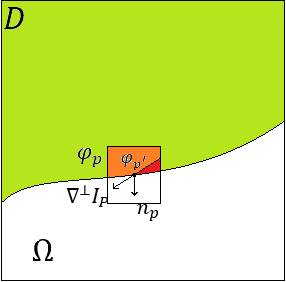
\includegraphics[scale=0.6]{rysunki/4_fig3}
	\caption{Oznaczenie wektorów wykorzystywanych do liczenia wartości $D(x)$. Rysunek autorski.}
	\label{4_fig3} 
\end{figure}
Zgodnie z \autoref{4_fig3} funkcja $D_t$ w sposób liczbowy określa z jaką siłą izolinia obrazu ${\mathrm{\nabla }}^{\bot }u_x$ dotyka granicy maski. Siła ta zależy również od wektora normalnego i jest największa gdy oba wspomniane wektory normalny i wektor izolinii są do siebie równoległe (zgodnie z iloczynem skalarnym wektorów ${\mathrm{cos} \ 0^0\ }=1)$.
W przeciwieństwie do definicji składnika $C_t$ funkcję $D_t$ można zinterpretować jako człon odpowiedzialny za przyznanie wyższego priorytetu pikselowi, stanowiącemu część struktury, która według wyników badań z zakresu psychologii widzenia powinna być kontynuowana w głąb odrestaurowywanego obszaru. Funkcja $D_t$ wpływa na zmniejszenie pojawiającego się w metodzie zjawiska wprowadzania niespójności obrazu. Niech funkcja $f(p)$ w punkcie obrazu $p \in D \cup \Omega \ $, gdzie $C(p) > 0$ przyjmuje wartość 0, a w punktach $C(p) = 0$ niech funkcja ta przyjmuje wartość 1, $f : (\Omega \cup D \to \{0,1\}$.  Wtedy korzystając z zależności \eqref{dfdx} i \eqref{dfdy} wektor normalny do granicy maski możemy wyznaczyć z następujących równań:
\begin{align}
n_p= \left[-n_{p_x}\frac{1}{l}\ ,\ -n_{p_y} \frac{1}{l}\right] =\left[-\frac{f_{i+1,j}+f_{i-1,j}}{2h}\cdot \frac{1}{l}, \  -\frac{f_{i,j+1} + f_{i,j-1}}{2h} \cdot \frac{1}{l}\right],
\label{KIERUNEK}
\end{align}
\begin{align}
l= \sqrt{n^2_{p_x} + n^2_{p_y}}.
\label{POMKIERUNEK}
\end{align}
Dyskretyzacja równania \eqref{DataTerm} zgodnie z \eqref{u}, \eqref{v}, \eqref{KIERUNEK} i \eqref{POMKIERUNEK} prowadzi do następującego równania:
\begin{align}
D(p)=\ \left|u{\cdot n}_x\frac{1}{L}-v\cdot n_y\frac{1}{L}\right|.
\end{align}
Znając wartości $C_t\left(x\right)$ oraz $D_t(x)$ dla każdego piksela z granicy maski można wyznaczyć wartość priorytetów $P(x)$. Na ich podstawie wybierane jest okno $p(x)$, a następnie najlepsze odwzorowanie $q_{\hat{x}}$.
Podsumowując operację wmalowywania obrazu można przedstawić w postaci następującego algorytmu. Algorytm ten należy powtarzać aż do wypełnienia wszystkich pikseli z $\mathrm{\Omega }$:
\begin{enumerate}
\item
Na podstawie \eqref{LAPLASJAN} wyznaczamy granicę maski $\mathrm{\partial }\mathrm{\Omega }$.
\item
Na podstawie \eqref{PRIORITY} wyznaczamy priorytety wszystkich pikseli z granicy maski $\mathrm{\partial }\mathrm{\Omega }$.
\item
Na podstawie \eqref{FROBENIUS} wyznaczamy najlepsze dopasowanie dla okna utworzonego na podstawie punktu drugiego.
\item
Zgodnie z \autoref{4_fig1} przepisujemy wartości z okna najlepszego dopasowania w restaurowany obszar.
\end{enumerate}
\section{Pojęcie głównych struktur.}
\label{sec:crimMetodSalient}
\subsection{Manualne definiowanie struktur.}
Poprawa algorytmu przedstawiona w \cite{criminisi2004region} prowadzi do polepszenia otrzymywanych wyników, lecz nie w optymalnym stopniu. W celu dalszej minimalizacji uzyskiwanych niespójności w obrazie i optymalizacji pod kątem szybkości działania algorytmów zostały wprowadzone kolejne modyfikacje: \cite{StructurePropagationManual},  \cite{malluvalasaimplementation}, \cite{SalientStrucTexProp}. 
Jednym z istotnych ulepszeń algorytmu wmalowywania w oparciu o kopiowanie fragmentów jest wprowadzenie zależności kolejności ich wstawiania w oparciu o główne struktury w obrazie.
Różnica pomiędzy algorytmem przedstawionym w \cite{criminisi2004region}, a algorytmem opisanym w \cite{StructurePropagationManual} polega na wstępnej definicji przez użytkownika grupy punktów znajdujących się w masce. Najczęściej są to krzywe, które zgodnie z psychologią widzenia powinny być kontynuowane w głąb maski tworząc odpowiednie połączenia między sobą. Krzywe te charakteryzują się ograniczoną grupą pikseli mogących stanowić źródło uzupełniania maski. Ograniczając pole obszaru $D^c$ dla każdej kontynuowanej krzywej (a najczęściej dla pary łączonych krzywych) znacząco przyspiesza się krok iteracji związany z odnalezieniem najlepszego dopasowania $p_x$ oraz $q_{\hat{x}}$. Schemat wmalowywania w oparciu o powyższy algorytm przedstawia \autoref{4_fig4}.
\begin{figure}[!h]
	\centering
	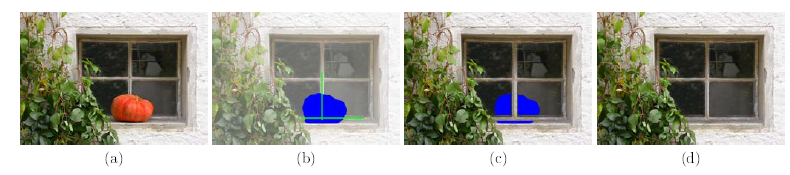
\includegraphics[scale=1.1]{rysunki/4_fig4}
	\caption{Koncepcja wmalowywania w oparciu o główne struktury obrazu. Źródło \cite{StructurePropagationManual}.}
	\label{4_fig4} 
\end{figure}
\textbf{W niniejszej pracy zaimplementowano i sprawdzono odrestaurowywanie obrazu na podstawie zadawanych ręcznie przez użytkownika głównych linii zgodnie z procedurą opisaną w  \cite{StructurePropagationManual}.}
\subsection{Automatyczne wykrywanie struktur.}
\textbf{Autor niniejszej pracy podjął się również implementacji w pełni automatycznego programu do procesu wmalowywania opierającego się na metodzie przedstawionej w publikacji \cite{SalientStrucTexProp}}. Zaproponowano tam  dodatkową analizę obrazu ograniczającą interakcję użytkownika wyłącznie do wprowadzenia maski. Autorzy wspomnianej publikacji proponują wykonać dwa dodatkowe kroki:
\begin{enumerate}
\item
Wyznaczyć główne struktury obrazu.
\item
Rozwiązać następujące zależności:
\begin{align}
D(i,j)\triangleq IP\cdot \left[\alpha \cdot D_1\left(f^i_C,f^j_C\right)\ +\ \beta {\cdot D}_2\left(f^i_T,f^j_T\right)+\gamma {\cdot D}_3\left(f^i_{Cur},f^j_{Cur}\right)\right],
\label{SalientDistance}
\end{align}
\begin{align}
Paired\left(i,j\right)={\mathrm{arg}\ \mathop{\mathrm{min}}_{i,j\ \epsilon \mathrm{\ }\{1,..,N\}} D(i,j)\ },
\label{SalientPair}
\end{align}
\end{enumerate}
gdzie człon $IP$ określa czy para głównych struktur $(i,j)$ jest do siebie równoległa, czy nie, $D_1$ to liczbowa reprezentacja podobieństwa kolorów, $D_2$ to liczbowa reprezentacja podobieństwa tekstur, a $D_3$ to liczbowa reprezentacja podobieństwa krzywizn. 
Analiza powyższych równań zostanie wykonana w sposób szczegółowy dla każdego z członów $\alpha \cdot D_1\left(f^i_C,f^j_C\right)\ $,$\ \beta {\cdot D}_2\left(f^i_T,f^j_T\right)$, oraz $\gamma {\cdot D}_3\left(f^i_{Cur},f^j_{Cur}\right)$. Krokiem wstępnym do rozwiązania powyższych równań według \cite{SalientStrucTexProp} jest wyznaczenie głównych struktur na podstawie obrazu wejściowego poddanego wstępnemu rozmyciu funkcją Gauss'a:
\begin{align}
G\left(i,j\right)=\frac{1}{\sqrt{2\pi }\sigma }e^{\frac{i^2+j^2}{2{\sigma }^2}}.
\label{rozmycieGaussa}
\end{align}
Operacji rozmycia dokonuje się poprzez operację splotu obrazu z odpowiednio wygenerowaną macierzą wyznaczoną na podstawie powyższego równania. Operacja rozmycia pozwala pozbyć się mniej znaczących krawędzi z obrazu zostawiając tylko najistotniejsze cechy, które powinny być kontynuowane w niewyznaczonym obszarze. Po operacji rozmycia autorzy w \cite{SalientStrucTexProp} proponują wykrycie głównych struktur na podstawie transformacji falkowej oraz odpowiednio wyznaczonych lokalnych maksimów dla funkcji powstałych na podstawie wspomnianej transformacji. Po tak  przeprowadzonej operacji uzyskuje się wszystkie główne struktury obrazu. Zbiorem krawędzi poddanych analizie są ostatecznie struktury, dla których dochodzi do przecięcia ze zdefiniowaną maską $\mathrm{\Omega }$ zgodnie z \autoref{4_fig5} (jako maska traktowany jest samochód).
\begin{figure}[!h]
	\centering
	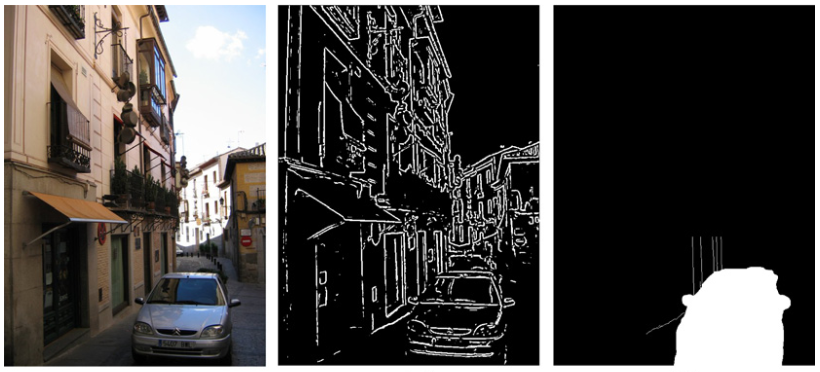
\includegraphics[scale=0.8]{rysunki/4_fig5}
	\caption{Koncepcja wmalowywania w oparciu o główne struktury obrazu. źródło \cite{StructurePropagationManual}.}
	\label{4_fig5} 
\end{figure}
Dla każdej linii stykającej się z obszarem $\mathrm{\Omega }$ wyznaczony zostaje punkt środkowy. Względem środka tego punktu tworzone jest okno  $f^i$ o wcześniej zdefiniowanym obszarze. Pierwszym członem w równaniu \eqref{SalientDistance} wyznaczonym na podstawie utworzonego okna $f^i$ jest $D_1\left(f^i_C,f^j_C\right)$. Symbole $f^i_C$ oraz $f^j_C$ stanowią posegmentowane fragmenty obrazu względem wcześniej zdefiniowanej liczby głównych, dominujących kolorów w obrazie. Dla każdego wycinka $f^i_C$ można zdefiniować zbiór punktów $(c_k,p_k)$, gdzie $c_k$ odpowiada danemu kolorowi, natomiast $p_k$ jego procentowemu udziałowi we fragmencie $f^i$, przy $k=1,\dots ,M$. Dysponując zbiorami punktów dla okien $f^i_C$,$\ f^j_C$ można liczbowo przedstawić ich poziom podobieństwa obliczając \cite{chen2005adaptive}:
\begin{align}
D_1\left(f^i_C,f^j_C\right)=IOCCD({\left(c_k,p_k\right)}_i,{\left(c_k,p_k\right)}_j,
\label{colDistance}
\end{align}
czyli obliczając normę $IOCCD$, z ang. improved optimal color composition distance, która to reprezentuje liczbowo stopień podobieństwa okien na podstawie kompozycji kolorystycznej.
Dokładna analiza oraz sposób wyznaczania podobieństwa okien $f^i$ przedstawione są w pozycji \cite{chen2005adaptive}.
Drugim członem w równaniu \eqref{SalientDistance} jest $D_2\left(f^i_T,f^j_T\right)$ określające stopień podobieństwa tekstur znajdujących się w utworzonych oknach $f$. Dla każdego obszaru $f^i$ wyznaczana jest macierz $MR8(f^i)$. Macierz uzyskiwana jest na podstawie odpowiedzi wybranego fragmentu obrazu na grupę 38 filtrów przedstawionych na \autoref{4_fig6}.
\begin{figure}[!h]
	\centering
	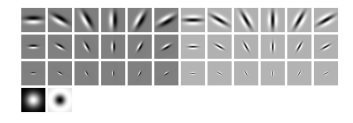
\includegraphics[scale=1.7]{rysunki/4_fig6}
	\caption{Bank 38 filtrów grupy MR8. źródło \cite{varma2009statistical}.}
\label{4_fig6}
\end{figure}
Przez odpowiedź obrazu na filtr należy rozumieć operację splotu z macierzą odpowiadającą definicji konkretnego filtru. W grupie filtrów $MR8$ branych pod uwagę znajduje się filtr Gauss'owski, oraz filtr $LOG$ będący laplasjanem funkcji Gauss'owskiej.
Na pozostałe 36 filtrów składają się dwie grupy filtrów utworzonych na podstawie filtru krawędziowego oraz filtru (w języku angielskim) "bar filter". Każdy z nich przedstawiony jest w sześciu orientacjach oraz trzech skalach zgodnie z \autoref{4_fig6}. Maksymalna odpowiedź na bazę trzydziestu ośmiu filtrów definiowana jest następująco:
\begin{align}
I_{fmax}(p)=\mathrm{max}\big[(I_{f1}(p),I_{f2}(p),\dots ,I_{f38}(p) \big],
\end{align}
gdzie $p$ - piksel obrazu poddanego filtracji, $p\in I$, $I_{fi}$ - odpowiedź obrazu $I$ na $i$-ty filtr z bazy filtrów. Wzajemne podobieństwo wyznaczonych okien odpowiadających głównym strukturom w obrazie można wyrazić zależnością:
\begin{align}
D_2{\left(f^i_T,f^j_T\right)}_i=\frac{{\left|MR8\left(f^i\right)-MR8\left(f^j\right)\right|}_F}{250}=\frac{{\left|f^i_T-f^j_T\right|}_F}{250}.
\end{align}
W przedstawionej zależności norma oznaczona literą $F$ oznacza normę Frobeniusa liczoną zgodnie z \eqref{FROBENIUS}.
Dokładny algorytm klasyfikacji tekstur przedstawiony został przez Manika Varma'e i Adrew Zisserman'a w \cite{varma2009statistical}. Ostatnim członem w równaniu \eqref{SalientDistance} jest człon $D_3\left(f^i_{cur},f^j_{cur}\right)$ odpowiadający liczbowej reprezentacji podobieństwa krzywizn ze zbioru głównych struktur. Autorzy w \cite{SalientStrucTexProp} nie podają jednak sposobu wyznaczenia normy:
\begin{align}
D_3\left(f^i_{cur},f^j_{cur}\right)=\ \left|curvature_i-curvature_j\right|.
\end{align}
Proponują oni natomiast aby każdą z wyznaczonych głównych struktur obrazu przedstawić w postaci równania wielomianu drugiego stopnia. Aproksymacji współczynników wielomianu można dokonać na podstawie rozwiązania następującego równania macierzowego:
\begin{align}
\left[ \begin{array}{ccc}
n & \sum{x_i} & \sum{x^2_i} \\ 
\sum{x_i} & \sum{x^2_i} & \sum{x^3_i} \\ 
\sum{x^2_i} & \sum{x^3_i} & \sum{x^4_i} \end{array}
\right]\cdot \left[ \begin{array}{c}
a_0 \\ 
a_1 \\ 
a_2 \end{array}
\right]=\left[ \begin{array}{c}
\sum{y_i} \\ 
\sum{x_iy_i} \\ 
\sum{{x^2_iy}_i} \end{array}
\right],
\end{align}
gdzie $n$ określa liczbę zastosowanych par $(x_i,y_i)$, a wielomian przedstawia się w postaci:
\begin{align}
curvature_i={f_i\left(x\right)=a}_{0_i}+a_{1_i}x+a_{2_i}x^2.
\end{align}
Według wyznaczonych równań, pary głównych struktur uzyskane w dalszych krokach algorytmu, propagowane są w głąb obszaru $\mathrm{\Omega }$, aż do momentu ich przecięcia. Ostatnią ważną zmienną w równaniu \eqref{SalientDistance} jest $IP$. Jest to zmienna, która przyjmuje wartość zerową, gdy badana para głównych struktur nie jest do siebie równoległa, bądź przyjmuje wartość jeden w przeciwnym wypadku. Aby uzyskać równania prostych opisujące wyznaczone krzywe można dokonać aproksymacji na podstawie transformacji Hough'a. Transformacja ta bazuje na następującej postaci równania prostej:
\begin{align}
y=\ -\frac{{\mathrm{cos} \theta \ }}{{\mathrm{sin} \theta \ }}x+\frac{r}{{\mathrm{sin} \theta \ }}.
\label{HOUGHTRANSFORM}
\end{align}
Posługiwanie się parametrami $\theta $ oraz $r$ pozwala uniknąć niejednoznaczności, w przypadku opisu linii pionowych oraz umożliwia przedstawienie prostej w postaci jednego punktu w przestrzeni Hough'a. Przekształcenie z przestrzeni $D^c$ można przedstawić następująco:
\begin{figure}[!h]
	\centering
	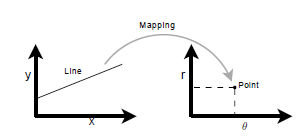
\includegraphics[scale=1.35]{rysunki/4_fig7}
	\caption{Odwzorowanie prostej w przestrzeni Hough’a. Źródło \cite{houghTransform}}.
\label{4_fig7}
\end{figure}
Posługując się parametrem $\theta$ określającym kąt pomiędzy wyznaczoną prostą a osią $x$ łatwo określić czy badane proste są do siebie równoległe. Aby wyznaczyć parametry prostej z równania \eqref{HOUGHTRANSFORM} zgodnie z \cite{houghTransform} należy każdemu punktowi tworzącemu prostą przypisać grupę punktów z przestrzeni Hough'a dla których wszystkie możliwe proste utworzone na ich podstawie zawierałyby badany punkt. Ostatecznie parametry prostej pochodzą z punktu, dla którego w przestrzeni Hough'a występuje największa gęstość powtarzających się punktów. Transformację przedstawia \autoref{4_fig8}:
\begin{figure}[!h]
	\centering
	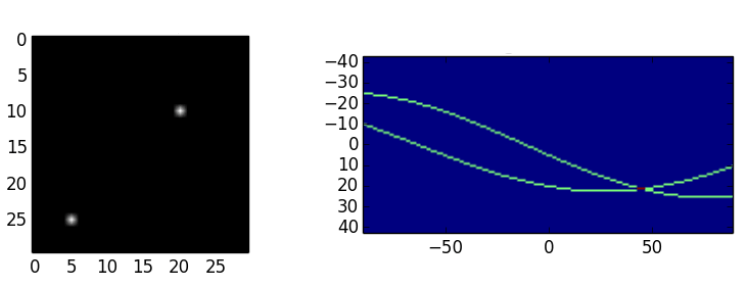
\includegraphics[scale=0.65]{rysunki/4_fig8}
	\caption{Transformacja dwóch punktów do dwóch krzywych w przestrzeni Hough'a. Punkt przecięcia definiuje prostą zawierającą dwa punkty (wygenerowano za pomocą programu Matlab).}
\label{4_fig8}
\end{figure}
Dokładną analizę transformacji można znaleźć w \cite{houghTransform}.
Pojawiające się współczynniki $\alpha ,\beta ,\gamma $ w równaniu \eqref{SalientDistance} stanowią wcześniej zdefiniowane wartości przypisujące procentowy wpływ poszczególnych członów na ostateczną wartość dopasowania $D(i,j)$. Według \cite{SalientStrucTexProp} najważniejszym dopasowaniem jest dopasowanie kolorów, następnie tekstur i krzywizn. Stąd należy przyjmować $\alpha >\beta >\gamma $ gdzie suma współczynników wynosi 1. \textbf{W pracy zbadano powyższe rozwiązanie w ograniczeniu do wykorzystania członów $D_1\left(f^i_C,f^j_C\right)$ oraz $IP$}. Człon $D_2\left(f^i_T,f^j_T\right)$ jest istotny w przypadku obrazów monochromatycznych o różnej teksturze. \textbf{Autor niniejszej pracy zauważa, że w przypadku obrazów kolorowych w większości przypadków linie granicy głównych struktur tworzone są poprzez gradienty kolorów}.
\chapter{Autorska modyfikacja algorytmów}
\section{Modyfikacja algorytmu bazującego na równaniu Naviera-Stokesa}
\subsection{Dyskretyzacja dyfuzji anizotropowej}
\label{ssec:anisModNS}
Jedną z głównych niedogodności rozwiązania opartego na równaniu mechaniki płynów jest konieczność przyjęcia takich parametrów, dla których uzyskuje się jednocześnie stabilność, sprawność obliczeń oraz odpowiednią dokładność rozwiązania (ograniczenie rozmycia uzyskanego obrazu). Implementacja równania \eqref{NavierAdv} według oryginalnie przedstawionego w publikacji \cite{au2001image} sposobu dyskretyzacji, nie pozwala wpłynąć na uzyskiwany ostatecznie wynik pomimo wielu prób parametryzacji. To skłoniło autora ninijszej pracy do zmiany sposobu dyskretyzacji na sposób przedstawiony w \cite{van2005algorithms}. Algorytm ten wykorzystuje asymetryczny schemat liczenia pierwszej pochodnej funkcji. Niech pierwsze pochodne lewostronne przyjmą postać:
\begin{equation}
\frac{\partial^-f}{\partial x}\bigg|_{i,j}=\frac{f_{i,j}-f_{i-1,j}}{\Delta x}
\label{leftdfdx}
,
\end{equation}
\begin{equation}
{\frac{{\partial }^-f}{\partial y}}\bigg|_{i,j}=\frac{f_{i,j}-f_{i,j-1}}{\Delta y}
\label{leftdfdy}
\end{equation}
i analogicznie pochodne prawostronne zapiszmy jako:
\begin{equation}
{\frac{{\partial }^+f}{\partial x}}\bigg|_{i,j}=\frac{f_{i+1,j}-f_{i,j}}{\Delta x} 
\label{rightdfdx}
,
\end{equation}
\begin{equation}
{\frac{{\partial }^+f}{\partial y}}\bigg|_{i,j}=\frac{f_{i,j+1}-f_{i,j}}{\Delta y}
\label{rightdfdy}
.
\end{equation}
Zależności te znajdą zastosowanie w wyznaczeniu wyrażeń
${\partial }_y \Big(g\left(\left|\nabla \omega \right|\right){\partial }_y\omega \Big)$ oraz
${\partial }_x\Big(g\left(\left|\nabla \omega \right|\right){\partial }_x\omega \Big)$. Stosując naprzemiennie schemat lewostronny i prawostronny do liczenia wartości pochodnych wewnętrznych i zewnętrznych w wyniku otrzymujemy ogólny schemat centralny. Zatem ostatecznie równanie \eqref{NavierAdv} można przedstawić w następującej postaci dyskretnej:
\begin{align}
\begin{aligned}
{\left\{ad\right\}}_{i,j}
&= \frac{1}{2}\biggl[\left(g_{i,j}+g_{i+1,j}\right)\left({\omega }_{i+1,j}-{\omega }_{i,j}\right) -\\[1ex]
&- \left(g_{i-1,j}+g_{i,j}\right)\left({\omega }_{i,j}-{\omega }_{i-1,j}\right) +  \\[1ex]
&+ \left(g_{i,j}+g_{i,j+1}\right)\left({\omega }_{i,j+1}-{\omega }_{i,j}\right) -\\[1ex]
&- \left(g_{i,j-1}+g_{i,j}\right)\left({\omega }_{i,j}-{\omega }_{i,j-1}\right)\biggl].
\end{aligned}
\label{discreteAnisotropic2}
\end{align}
\subsection{Algorytm wmalowywania tekstury obrazu}
Jednym ze sposobów wmalowywania jest osobne rozpatrywanie uzyskanej w wyniku segmentacji struktury i tekstury obrazu. \textbf{Autor niniejszej pracy proponuje wypełnianie tekstury w oparciu o metodę Criminisi'ego opisaną w podrozdziale \ref{sec:crimMetod}} zamiast stosowania metody przedstawionej na rysunku \ref{5_fig1}.
\section{Modyfikacja algorytmu Criminisi.}
\label{ssec:crimMod}
\subsection{Modyfikacja źródła czerpania dopasowania.}
\label{ssec:crimModSource}
W niniejszej pracy algorytm wypełniania fragmentami obrazu zmieniono przez wprowadzenie okna poszukiwania $r_x$, będącego otoczeniem piksela $x$ z bokiem o długości $r$. Wprowadzone okno ogranicza zbiór pikseli, dla których tworzony jest fragment obrazu $q_{\hat{x}}$ porównywany z $p_{x}$.
Piksel $\hat{x}$ przedstawimy jako $\hat{x} \in r_x$, a zbiór $r_x$ jako 
$\forall \ \hat{x} \in r_x: \forall \ p \in q_{\hat{x}} \cap \ \Omega = \emptyset$. Zapisując formalnie - wprowadzamy dodatkową funkcję $f_r$ tworzącą dla każdego piksela $x$ podzbiór $r_x$:
\begin{align}
r_x = f_r(x).
\end{align}
Takie zmniejszenie pozwala ograniczyć czas odnalezienia najlepszego wzorca \eqref{FROBDIST} - $|s_x| > |r_x|$. Zmniejszenie okna poszukiwania pozwala także poprawić jednolitość uzyskiwanych struktur. Na rysunku \ref{4_fig9}, dla piksela $p$ podczas wyznaczania najlepszego dopasowania \eqref{FROBDIST} prawdopodobieństwo wstawienia piksela z ze strukury obcej, np. 1 czy 4, jest mniejsze.
\begin{figure}[!h]
	\centering
	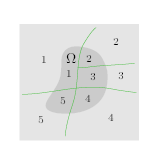
\includegraphics[scale=0.4]{rysunki/4_fig9}
	\caption{Grupowanie podzbiorów stanowiących źródło fragmentów wykorzystywanych do syntezy podzbiorów nieznanego obszaru $\boldsymbol{\mathrm{\Omega }}$. Rysunek autorski.}
\label{4_fig9}
\end{figure}
\subsection{Modyfikacja sposobu wyznaczania podobieństwa.}
\label{ssec:modDistForCrim}
W niniejszej pracy przetestowano różne rodzaje odległości $d\left( u(p_x), \hat{u} (q_{\hat{y}}) \right)$  zastępując oryginalną odległosć wprowadzoną przez autorów w \cite{criminisi2004region} definicję \eqref{FROBENIUS2} równaniami: \eqref{NLWEIGHT}, \eqref{normNNF}, \eqref{nonLocalMeans}, \eqref{nonLocalMedians} oraz \eqref{nonLocalpoisson}.
\subsection{Modyfikacja funkcji $D_t$.}
\label{ssec:modDtForCrim}
Granicę maski $\partial \mathrm{\Omega }$ wyznacza się wykorzystując operację erozji i dylacji. Innym sposobem jest zastosowanie dyskretnego splotu maski z macierzą reprezentującą laplasjan dla siatki 8-spójnej: 
\begin{equation}
s_8 = 
\left[ \begin{array}{ccc}
1 & 1 & 1 \\ 
1 & -8 & 1 \\ 
1 & 1 & 1 \end{array}
\right]
\label{LAPLASJAN}
.
\end{equation}
Poprawę dokładności wyznaczania wektorów $n_x$ oraz $\nabla^\bot u_x$ (\autoref{4_fig3}) wnikających wgłąb nieznanego obszaru, a więc i poprawę dokładności algorytmu, w niniejszej pracy uzyskuje się przez uwzględnienie różniczek wyznaczanych dla wszystkich pikseli stanowiących otoczenie głównego piksela $x$. Wpływ każdej z różniczek na ostatecznie wyznaczaną wartość jest procentowo określany.
Na przykład niech otoczenie piksela $(i, j)$ stanowi macierz o rozmiarze $3 \times 3$. Wtedy jeśli chcemy wyznaczyć $n_{p_{(i,j)}}$ zastosujemy równanie:
\begin{equation}
\begin{bmatrix}
n_{p_{(i,j)}}
\end{bmatrix}
=\frac{1}{2h}
\cdot
\begin{bmatrix}
-1 & 0 & 1
\end{bmatrix}
\cdot
\begin{bmatrix}
f_{i-1, j-1} & f_{i-1, j} & f_{i-1, j+1}\\ 
f_{i,   j-1} & f_{i,   j} & f_{i,   j+1}\\
f_{i+1, j-1} & f_{i+1, j} & f_{i+1, j+1}
\end{bmatrix}
\cdot
\begin{bmatrix}
c_1\\ 
c_2\\
c_3
\end{bmatrix},
\end{equation}
gdzie $c_1, c_2, c_3$ oznaczają współczynniki stopniujące wpływ różniczek (mogą być wyznaczane na podstawie rozkładu Gauss'a). Analogicznie postępujemy dla innych rozmiarów.
\section{Model NLCTV}
\label{sec:smodNLCTV}
\subsection{Modyfikacja funkcji wagi.}
W trakcie testowania algorytmu pożądanym przez Autora tej pracy magisterskiej stało się poszerzenie zbyt lokalnej analizy obrazu, skutkującej nieodpowiednią kontynuacją struktury. Zwiększanie parametrów wejściowych takich jak rozmiar fragmentu obrazu $p_x$ i rozmiar okna $\text{N}_x$ powoduje, że struktury w uzyskiwanych wynikach stają się coraz bardziej rozmyte, połączone ze sobą. Wypełniony obraz nie posiada także tekstury. Aby uniknąć tego zjawiska Autor tej pracy zaproponował modyfikację funkcji wagi \eqref{NLWEIGHT} do następującej postaci:
\begin{align}
\begin{aligned}
w\left(x,y\right) &= {\mathrm{exp} \left\{-\frac{G_{\sigma }*{\big|I\left(x+\ \cdot \right)-I\left(y+\ \cdot \right)\big|}^2}{r^2}\right\} \cdot}\\
&\cdot {\mathrm{exp} \left\{-\frac{G_{\sigma }*{\Big|I\big(x+\ s(\cdot) \big)-I\big(y+\ s(\cdot) \big)\Big|}^2}{r^2}\right\} }.
\label{NLWEIGHTMODIFIED}
\end{aligned}
\end{align}
W przytoczonej zależności człon $s(\cdot)$ oznacza przeskalowanie  domyślnej wartości przyjętego rozmiaru fragmentu obrazu do rozmiaru $s$-krotnie większego. Edycja nie dotyczy pozostałej części  algorytmu i wpływa jedynie na wartość obliczanej wagi.
\section{Połączenie syntezy obrazu z funkcją wagi.}
Kolejną modyfikacją algorytmu $NLCTV$ wykonaną przez Autora tej pracy jest zastąpienie równania \eqref{NLH1}, metodą syntezy obrazu bazującej na metodzie syntezy tekstury. Kroki nowego algorytmu można wtedy przedstawić w następującym schemacie postępowania:
\begin{enumerate}
\item
Wyznaczeniu funkcji wagi $w$ zgodnie z zależnością \eqref{DNLWEIGHT}.
\item
Powtarzaniu aż do uzyskania zbioru $\Omega = \emptyset$ następujących czynności:
\begin{itemize}
\item
znajdowania dla każdego $x \in \partial\Omega$ najlepszego dopasowania $\hat{x} \in D \cap \mathrm{N}_x$:
\begin{large}
\begin{align}
\hat{x} = \mathop{\mathrm{arg \ max}}_{p \in D \cap \mathrm{N}_x} w(x,\hat{x}),
\end{align}
\end{large}
a następnie przypisania:
\begin{align}
u(x) = \hat{u}(\hat{x}),
\end{align}
\item
i pomniejszenia maski $\Omega$ o granicę $\partial\Omega$.
\end{itemize}
\end{enumerate}
\chapter{Testy algorytmów}
\section{Analizowane obrazy.}
W niniejszej pracy testom poddano następującą grupę obrazów:
\begin{longtable}[h!]{|c|c|}
    \hline
    Obraz & Dane \\ \hline

    \begin{minipage}{.65\textwidth}
    \vspace{0.2cm}
    \centering
    \includegraphics[height=5.8cm]{imgmask/kotmyszm}
    \vspace{0.2cm}
    \end{minipage}
    &
    \begin{minipage}{.35\textwidth}
    \begin{tabular}{ l l  }
		Wymiar: & 500 $\times$ 375 \\
		Udział maski: &  28\% \\
		Nazwa: & \fullkotmyszm
    \end{tabular}
    \end{minipage} \\ \hline
    
    \begin{minipage}{.65\textwidth}
    \vspace{0.2cm}
    \centering
    \includegraphics[height=5.8cm]{imgmask/maciek1m}
    \vspace{0.2cm}
    \end{minipage}
    &
    \begin{minipage}{.35\textwidth}
    \begin{tabular}{ l l  }
	Wymiar: & 410 $\times$ 308 \\
	Udział maski: & 28\% \\
	Nazwa: & \fullmaciekIm
    \end{tabular}
    \end{minipage} \\ \hline
    
    \begin{minipage}{.65\textwidth}
    \vspace{0.2cm}
    \centering
    \includegraphics[height=5.8cm]{imgmask/Obr1m}
    \vspace{0.2cm}
    \end{minipage}
    &
    \begin{minipage}{.35\textwidth}
    \begin{tabular}{ l l  }
	Wymiar: & 614 $\times$ 461 \\
	Udział maski: & 9\% \\
	Nazwa: & \fullObrIm
    \end{tabular}
    \end{minipage} \\ \hline
    
    \begin{minipage}{.65\textwidth}
    \vspace{0.2cm}
    \centering
    \includegraphics[height=5.8cm]{imgmask/Obr4m}
    \vspace{0.2cm}
    \end{minipage}
    &
    \begin{minipage}{.35\textwidth}
    \begin{tabular}{ l l  }
	Wymiar: & 576 $\times$ 360 \\
	Udział maski: & 7\% \\
	Nazwa: & \fullObrIVm
    \end{tabular}
    \end{minipage} \\ \hline

    \begin{minipage}{.65\textwidth}
    \vspace{0.2cm}
    \centering
    \includegraphics[height=5.8cm]{imgmask/Obr5m}
    \vspace{0.2cm}
    \end{minipage}
    &
    \begin{minipage}{.35\textwidth}
    \begin{tabular}{ l l  }
	Wymiar: & 650 $\times$ 570 \\
	Udział maski: & 28\% \\
	Nazwa: & \fullObrVm
    \end{tabular}
    \end{minipage} \\ \hline

    \begin{minipage}{.65\textwidth}
    \vspace{0.2cm}
    \centering
    \includegraphics[height=6.8cm]{imgmask/Obr6m}
    \vspace{0.2cm}
    \end{minipage}
    &
    \begin{minipage}{.35\textwidth}
    \begin{tabular}{ l l  }
	Wymiar: & 655 $\times$ 491 \\
	Udział maski: & 9\% \\
	Nazwa: & \fullObrVIm
    \end{tabular}
    \end{minipage} \\ \hline
    
    \begin{minipage}{.65\textwidth}
    \vspace{0.2cm}
    \centering
    \includegraphics[height=5.8cm]{imgmask/Obr15m}
    \vspace{0.2cm}
    \end{minipage}
    &
    \begin{minipage}{.35\textwidth}
    \begin{tabular}{ l l  }
	Wymiar: & 1772 $\times$ 1181 \\
	Udział maski: & 4.5\% \\
	Nazwa: & \fullObrXVm
    \end{tabular}
    \end{minipage} \\ \hline

    \begin{minipage}{.65\textwidth}
    \vspace{0.2cm}
    \centering
    \includegraphics[height=7cm]{imgmask/Obr17m}
    \vspace{0.2cm}
    \end{minipage}
    &
    \begin{minipage}{.35\textwidth}
    \begin{tabular}{ l l  }
	Wymiar: & 206 $\times$ 308 \\
	Udział maski: & 14\% \\
	Nazwa: & \fullObrXVIIm
    \end{tabular}
    \end{minipage} \\ \hline

    \begin{minipage}{.65\textwidth}
    \vspace{0.2cm}
    \centering
    \includegraphics[height=7cm]{imgmask/Obr19m}
    \vspace{0.2cm}
    \end{minipage}
    &
    \begin{minipage}{.35\textwidth}
    \begin{tabular}{ l l  }
	Wymiar: & 461 $\times$ 615 \\
	Udział maski: & 7\% \\
	Nazwa: & \fullObrXIXm
    \end{tabular}
    \end{minipage} \\ \hline

    \begin{minipage}{.65\textwidth}
    \vspace{0.2cm}
    \centering
    \includegraphics[height=5.8cm]{imgmask/Obr28km}
    \vspace{0.2cm}
    \end{minipage}
    &
    \begin{minipage}{.35\textwidth}
    \begin{tabular}{ l l  }
	Wymiar: & 820 $\times$ 615 \\
	Udział maski: & 28\% \\
	Nazwa: & \fullObrXXVIIIkm
    \end{tabular}
    \end{minipage} \\ \hline

    \begin{minipage}{.65\textwidth}
    \vspace{0.2cm}
    \centering
    \includegraphics[height=5.8cm]{imgmask/Osoba_drugam}
    \vspace{0.2cm}
    \end{minipage}
    &
    \begin{minipage}{.35\textwidth}
    \begin{tabular}{ l l  }
	Wymiar: & 2592 $\times$ 1944 \\
	Udział maski: & 28\% \\
	Nazwa: & \fullOsobaDrugam
    \end{tabular}
    \end{minipage} \\ \hline
    
    \begin{minipage}{.65\textwidth}
    \vspace{0.2cm}
    \centering
    \includegraphics[height=5.8cm]{imgmask/Obr13m}
    \vspace{0.2cm}
    \end{minipage}
    &
    \begin{minipage}{.35\textwidth}
    \begin{tabular}{ l l  }
	Wymiar: & 1181 $\times$ 1772 \\
	Udział maski: & 4\% \\
	Nazwa: & \fullObrXIIIm
    \end{tabular}
    \end{minipage} \\ \hline
    \caption{Obrazy poddane analizie.}
  \label{imgmasks}
\end{longtable}
\section{Równanie mechaniki płynu.}
\label{sec:NVResult}
\subsection{Rozwiązanie równania Naviera-Stokes'a.}
Przykładowe wyniki  przedstawia Tab. \ref{TabNavierStokes}. \textbf{Wyniki uzyskane przy zastosowaniu schematu centralnego opisanego przez równanie \eqref{NavierDiffAdvCen} w porównaniu z wynikami otrzymanymi z zastosowaniem schematu "do przodu" opisanego przez równanie \eqref{NavierDiffAdvFor} nie wykazują znaczących różnic}. W przypadku dyfuzji anizotropowej opisanej przez równanie \eqref{NavierAdv}  \textbf{przedstawione w pracy sposoby dyskretyzacji} nie minimalizują wystarczająco rozmycia w odrestaurowywanej masce i mają znikomy wpływ na dokładność wyznaczonego obrazu. Również modyfikacja Autora opisana w podrozdziale \ref{ssec:anisModNS} ma znikomy wpływ na dokładność wyznaczonego obrazu.
\textbf{W trakcie badań Autor niniejszej pracy zauważył, że rozmycie obrazu w znaczącym stopniu spowodowane jest zgrubną dokładnością rozwiązania równania \eqref{Poisson}}. Warto zaznaczyć, że równanie \eqref{DiscreteSOR} rozwiązywane jest w każdej iteracji i w każdej iteracji wprowadza rozmycie, im bliżej środka wypełnianego obszaru tym większe. Przykładowe wyniki w zależności od parametru $h$  przedstawia \autoref{SORMethod}. Jeśli $\Delta t <0.1$ w równaniu \eqref{NavierDiffAdvFor} to stabilność algorytmu jest zachowana przy wartościach $h \geq 0.9$. W celu uzyskania dokładniejszej kontynuacji struktury należy rozważyć bardziej zaawansowane algorytmy dyskretyzacji równania mechaniki płynów, na przykład metody opisane w \cite{tschumperle2006fast}. Kontynuacja obrazu na podstawie równania mechaniki płynów nie jest metodą gwarantującą poprawną kontynuację tekstury. 
\begin{longtable}[h!]{|c|c|}
	\hline
	Obraz & Dane \\ \hline
    \begin{minipage}{.65\textwidth}
    \vspace{0.2cm}
    \centering
    \includegraphics[height=5.8cm]{TESTY/NavierStokes/{Obr4m.pngITER_10000dt_0.015h_3pr_2tns_2021.6256}.png}
    \vspace{0.2cm}
    \end{minipage}
    &
    \begin{minipage}{.3\textwidth}
		\begin{tabular}{ l l }
		Wynik & \ObrIVmu \\
		$\Delta t$ & = 0.01 \\
		$h$ & = 3 \\
		$t$ & = 2021.63s
		\end{tabular}	
    \end{minipage}  \\ \hline

    \begin{minipage}{.65\textwidth}
    \vspace{0.2cm}
    \centering
    \includegraphics[height=7.5cm]{TESTY/NavierStokes/{Obr17m.pngITER_10000dt_0.015h_3pr_2tns_3225.3982}.png}
    \vspace{0.2cm}
    \end{minipage}
    &
    \begin{minipage}{.3\textwidth}
		\begin{tabular}{ l l }
			Wynik & \ \ObrXVIImu \\
			$\Delta t$ & = 0.01 \\
			$h$ & = 3 \\
			$t$ & = 3225.40s
		\end{tabular}	
    \end{minipage}  \\ \hline

    \begin{minipage}{.65\textwidth}
    \vspace{0.2cm}
    \centering
    \includegraphics[height=7.5cm]{TESTY/NavierStokes/{maciek1m.pngITER_10000dt_0.015h_3pr_2tns_1736.7717}.png}
    \vspace{0.2cm}
    \end{minipage}
    &
    \begin{minipage}{.3\textwidth}
		\begin{tabular}{ l l }
			Wynik & \maciekImu \\
			$\Delta t$ &= 0.01 \\
			$h$ &= 3 \\
			$t$ &= 1736.77s
		\end{tabular}	
    \end{minipage}  \\ \hline
	\caption{Wmalowywanie obrazów bazujące na metodzie zaczerpniętej z równań występujących w mechanice płynów.}
	\label{TabNavierStokes}
\end{longtable}

\begin{longtable}[h!]{|c|c|}
    \hline
		Obraz & Dane \\ \hline
    \begin{minipage}{.65\textwidth}
    \vspace{0.2cm}
    \centering
    \includegraphics[height=5.8cm]{TESTY/SOR/{SOR}.png}
    \vspace{0.2cm}
    \end{minipage}
    &
    \begin{minipage}{.3\textwidth}
		Przykładowy obraz oryginalny
    \end{minipage}
    \\ \hline
    \begin{minipage}{.65\textwidth}
    \vspace{0.2cm}
    \centering
    \includegraphics[height=5.8cm]{TESTY/SOR/{SORITER_1h_1}.png}
    \vspace{0.2cm}
    \end{minipage} 
    &
    \begin{minipage}{.3\textwidth}
		Wynik dla parametru $h=1$
    \end{minipage} \\ \hline

    \begin{minipage}{.65\textwidth}
    \vspace{0.2cm}
    \centering
    \includegraphics[height=5.8cm]{TESTY/SOR/{SORITER_1h_10}.png}
    \vspace{0.2cm}
    \end{minipage}
    &
    \begin{minipage}{.3\textwidth}
		Wynik dla parametru $h=10$
    \end{minipage} \\ \hline
	\caption{Wyniki obrazów uzyskane metodą sukcesywnej nadrelaksacji (SOR), używanej w równaniu Naviera Stokesa (wpływ parametru $h$).}
	\label{SORMethod}
\end{longtable}
Dla większej wartości parametru $h$ uzyskuje się większą dokładność wyznaczonego obrazu. Niezależnie od dobrania parametru wynik generuje zjawisko rozmycia ostrych krawędzi obrazu.
\subsection{Segmentacja obrazu na strukturę i teksturę z wykorzystaniem metod Navier-Stokes'a i Criminisi.}
Przykłady obrazów poddanych segmentacji przedstawia \autoref{TabSegmentation}.\\
\begin{longtable}[h!]{|c|c|}
    \hline
    \multicolumn{2}{|c|}{
    	Segmentacja obrazu
    } \\ \hline
    \begin{minipage}{0.5\textwidth}
    \centering
	Obraz przed segmentacją
    \end{minipage}
	&
    \begin{minipage}{0.5\textwidth}
    \centering
	Wydzielona struktura obrazu
    \end{minipage}\\ \hline
    \multicolumn{2}{|c|}{
    \centering
    	$\lambda = 0.005$, $t=2.67s$, wynik \kotmyszmu
    } \\ \hline
    \begin{minipage}{0.5\textwidth}
    \vspace{0.2cm}
    \centering
    \includegraphics[height=5cm]{{imgmask/kotmyszm}.png}
    \vspace{0.2cm}
    \end{minipage}
	&
    \begin{minipage}{0.5\textwidth}
    \vspace{0.2cm}
    \centering
    \includegraphics[height=5cm]{{TESTY/SEGMENTACJA/kotmyszm.bmpUlambda_0.005ts_2.6707}.png}
    \vspace{0.2cm}
    \end{minipage}\\ \hline
    
    \multicolumn{2}{|c|}{
    \centering
    	$\lambda = 0.03$, $t=0.52s$, wynik \ObrXVIImu
    } \\ \hline
    \begin{minipage}{0.5\textwidth}
    \vspace{0.2cm}
    \centering
    \includegraphics[height=6cm]{{imgmask/Obr17m}.png}
    \vspace{0.2cm}
    \end{minipage}
	&
    \begin{minipage}{0.5\textwidth}
    \vspace{0.2cm}
    \centering
    \includegraphics[height=6cm]{{TESTY/SEGMENTACJA/Obr17m.pngUlambda_0.03ts_0.52276}.png}
    \vspace{0.2cm}
    \end{minipage}\\ \hline
    
    \multicolumn{2}{|c|}{
    \centering
    	$\lambda = 0.03$, $t=2.99s$, wynik \ObrIVmu
    } \\ \hline
    \begin{minipage}{0.5\textwidth}
    \vspace{0.2cm}
    \centering
    \includegraphics[height=4.5cm]{{imgmask/Obr4m}.png}
    \vspace{0.2cm}
    \end{minipage}
	&
    \begin{minipage}{0.5\textwidth}
    \vspace{0.2cm}
    \centering
    \includegraphics[height=4.5cm]{{TESTY/SEGMENTACJA/Obr4m.pngUlambda_0.03ts_2.9892}.png}
    \vspace{0.2cm}
    \end{minipage}\\ \hline
	\caption{Segmentacja obrazu na strukturę i teksturę.}
	\label{TabSegmentation}
\end{longtable}
Czas trwania segmentacji obrazu nie przekracza kilku sekund. Przy zmniejszaniu parametru $\lambda$ otrzymujemy większą gładkość wynikowej struktury obrazu. \textbf{W niniejszej pracy magisterskiej do syntezy struktury wykorzystano metodę Naviera-Stokesa, a do uzupełnienia tekstury metodę Criminisi}. Wyniki algorytmu przedstawia \autoref{TabNavierStokesSegm}. W tabeli Autor tej pracy magisterskiej porównuje wyniki z wynikami algorytmu bez wcześniejszej segmentacji obrazu.
\begin{longtable}[h!]{|c|c|}
    \hline
    \begin{minipage}{0.5\textwidth}
    \centering
	Metoda bez segmentacji
    \end{minipage}
	&
    \begin{minipage}{0.5\textwidth}
    \centering
	Metoda z segmentacją
    \end{minipage}\\ \hline


    \multicolumn{2}{|c|}{
    \centering
    Wyniki \ObrIVmu
    } \\ \hline

    \begin{minipage}{0.5\textwidth}
    \vspace{0.2cm}
    \centering
    \includegraphics[height=4.5cm]{TESTY/NavierStokes/{Obr4m.pngITER_10000dt_0.015h_3pr_2tns_2021.6256}.png}
    \vspace{0.2cm}
    \end{minipage}
	&
    \begin{minipage}{0.5\textwidth}
    \vspace{0.2cm}
    \centering
        Wynik \ObrIVmu
    \includegraphics[height=4.5cm]{{TESTY/NavierStokes/Obr4m.pngITER_16000dt_0.01h_1pr_2ts_0.37671tns_3310.8032tt_58.261}.png}
    \vspace{0.2cm}
    \end{minipage}\\ \hline

    \multicolumn{2}{|c|}{
    \centering
        Wyniki \ObrXVIImu
    } \\ \hline

    \begin{minipage}{0.5\textwidth}
    \vspace{0.2cm}
    \centering
    \includegraphics[height=7.5cm]{TESTY/NavierStokes/{Obr17m.pngITER_10000dt_0.015h_3pr_2tns_3225.3982}.png}
    \vspace{0.2cm}
    \end{minipage}
	&
    \begin{minipage}{0.5\textwidth}
    \vspace{0.2cm}
    \centering
    \includegraphics[height=7.5cm]{TESTY/NavierStokes/{Obr17m.pngdt_0.01h_1pr_3ts_0.49582tns_526.7624tt_26.033}.png}
    \vspace{0.2cm}
    \end{minipage}\\ \hline
	\caption{Porównanie wyników uzyskanych metodą rozwiązania równania Navier'a-Stokes'a do metody z algorytmem segmentacji.}
	\label{TabNavierStokesSegm}
\end{longtable}
Oddzielna synteza tekstury skutkuje jej kontynuacją wgłąb maski. W porównaniu z podrozdziałem \ref{sec:NVResult} \textbf{uzyskujemy nielokalny charakter rozwiązania}. Efekt rozmycia głównego algorytmu odrestaurowania struktury negatywnie wpływa na jakość obszaru wynikowego. Wynik tworzony z oddzielnie odrestaurowanej tekstury i struktury obrazu może prowadzić do powstania nieprawidłowych wyników w postaci nowych kolorów obrazu. Wadą algorytmu, co łatwo zauważyć w tabeli \ref{TabNavierStokesSegm} jest możliwość wstawienia do danej struktury obcej dla niej tekstury, pochodzącej z innej części obrazu.  W przypadku algorytmu dokonującego syntezy tekstury oddzielnie dla każdej z trzech segmentowanych warstw uzyskiwane wyniki również prowadzą do niepożądanego zjawiska tworzenia nowych kolorów w obrazie.
\subsection{Podsumowanie implementacji.}
Autor tej pracy magisterskiej sprawdził zaproponowane i opisane przez niego sposoby dyskretyzacji równań dyfuzji przy użyciu skryptów napisanych w Matlab'ie. \textbf{Do dalszych porównań metod bazujących na mechanice płynów (dyfuzji) z pozostałymi zaproponowanymi w tej pracy posłużono się implementacją zawartą w bibliotece OpenCV dostarczaną w ramach wolnego (ogólnodostępnego) oprogramowania.} Występuje tutaj dyskretyzacja dyfuzji oparta na równaniu przedstawionym w \cite{BertalmioNavierStokes} i zmniejsza efekt rozmycia stosując metodę przedstawioną w \cite{telea2004image}. Przykłady rozwiązań przedstawia tabela \ref{NavierStokesOpenCV}.
\begin{longtable}[h!]{|c|c|}
    \hline
    $t = 0.56$ s, wynik \maciekImu
    &
    $t = 0.62$ s, wynik \ObrXIXmu \\ \hline \hline

    \begin{minipage}{0.5\textwidth}
    \vspace{0.2cm}
    \centering
    
    \includegraphics[height=5.5cm]{{TESTY/OpenCV/Obr/maciek1}.png}
    \vspace{0.2cm}
    \end{minipage}
	&
    \begin{minipage}{0.5\textwidth}
    \vspace{0.2cm}
    \centering
    \includegraphics[height=6.5cm]{{TESTY/OpenCV/Obr/Obr19}.png}
    \vspace{0.2cm}
    \end{minipage} \\ \hline

    $t = 0.78$ s, wynik \ObrIVmu
    &
    $t = 0.44$ s, wynik \ObrXVIImu \\ \hline \hline

    \begin{minipage}{0.5\textwidth}
    \vspace{0.2cm}
    \centering
    \includegraphics[height=5cm]{{TESTY/OpenCV/Obr/Obr4}.png}
    \vspace{0.2cm}
    \end{minipage}
	&
    \begin{minipage}{0.5\textwidth}
    \vspace{0.2cm}
    \centering
    \includegraphics[height=7cm]{{TESTY/OpenCV/Obr/Obr17}.png}
    \vspace{0.2cm}
    \end{minipage} \\ \hline
	\caption{Rozwiązania uzyskane z wykorzystaniem biblioteki OpenCV, $ \ t$ - czas wmalowywania.}
	\label{NavierStokesOpenCV}
\end{longtable}
\textbf{Znaczna różnica w czasach wmalowywania obrazów} w głównej mierze (oprócz sposobu implementacji) spowodowana jest wolnym czasem wykonywania operacji matematycznych na macierzach w środowisku Matlab - w porównaniu do podstawowych implementacji w językach C/C++.
\section{Uzupełnianie kawałkami obrazu.}
\subsection{Metoda Criminisi.}
Przykładowe wyniki przedstawia tabela:
\begin{longtable}[h!]{|c|c|}
    \hline
    Obraz & Dane \\ \hline

    \begin{minipage}{.65\textwidth}
    \vspace{0.2cm}
    \centering
    \includegraphics[height=6.5cm]{TESTY/CRIM2004/Obr17/{Obr17m.pngpr_3sr_8006alfa_0.2t_31.7202}.png}
    \vspace{0.2cm}
    \end{minipage}
    &
    \begin{minipage}{.35\textwidth}
    \begin{tabular}{l l}
    	Wynik & \ObrXVIImu \\
         $|p_x|_r$:& 3 \\
         $t$: & 31.72s
    \end{tabular}
    \end{minipage} \\ \hline
    
    \begin{minipage}{.65\textwidth}
    \vspace{0.2cm}
    \centering
    \includegraphics[height=6.5cm]{TESTY/CRIM2004/Obr17/{Obr17m.pngpr_15sr_8006alfa_0.2t_22.4205}.png}
    \vspace{0.2cm}
    \end{minipage}
    &
    \begin{minipage}{.35\textwidth}
    \begin{tabular}{l l}
        	Wynik & \ObrXVIImu \\
         $|p_x|_r$: & 15 \\
         $t$: & 22.42s
    \end{tabular}
    \end{minipage} \\ \hline  
    
    \begin{minipage}{.65\textwidth}
    \vspace{0.2cm}
    \centering
    \includegraphics[height=6.5cm]{TESTY/CRIM2004/Obr17/{Obr17m.pngpr_23sr_8006alfa_0.2t_20.7783}.png}
    \vspace{0.2cm}
    \end{minipage}
    &
    \begin{minipage}{.35\textwidth}
    
    \begin{tabular}{l l}
        	Wynik & \ObrXVIImu \\
         $|p_x|_r$: & 23 \\
         $t$: & 20.77s
    \end{tabular}
    \end{minipage} \\ \hline
    
    \begin{minipage}{.65\textwidth}
    \vspace{0.2cm}
    \centering
    \includegraphics[height=4.7cm]{TESTY/CRIM2004/Obr4/{Obr4m.pngpr_3sr_8010alfa_0.2t_213.2492}.png}
    \vspace{0.2cm}
    \end{minipage}
    &
    \begin{minipage}{.35\textwidth}
    \begin{tabular}{l l}
    	Wynik & \ObrIVmu \\
         $|p_x|_r$: & 3 \\
         $t$: & 213.25s
    \end{tabular}
    \end{minipage} \\ \hline
    
    \begin{minipage}{.65\textwidth}
    \vspace{0.2cm}
    \centering
    \includegraphics[height=4.7cm]{TESTY/CRIM2004/Obr4/{Obr4m.pngpr_15sr_8010alfa_0.2t_113.4021}.png}
    \vspace{0.2cm}
    \end{minipage}
    &
    \begin{minipage}{.35\textwidth}
    \begin{tabular}{l l}
        	Wynik & \ObrIVmu \\
         $|p_x|_r$: & 15 \\
         $t$: & 113.40s
    \end{tabular}
    \end{minipage} \\ \hline  
    
    \begin{minipage}{.65\textwidth}
    \vspace{0.2cm}
    \centering
    \includegraphics[height=4.7cm]{TESTY/CRIM2004/Obr4/{Obr4m.pngpr_23sr_8010alfa_0.2t_134.3072}.png}
    \vspace{0.2cm}
    \end{minipage}
    &
    \begin{minipage}{.35\textwidth}
    \begin{tabular}{l l}
        	Wynik & \ObrIVmu \\
         $|p_x|_r$: & 23 \\
         $t$: & 134.31s
    \end{tabular}
    \end{minipage} \\ \hline
    
    \begin{minipage}{.65\textwidth}
    \vspace{0.2cm}
    \centering
    \includegraphics[height=6cm]{TESTY/CRIM2004/Obr19/{Obr19m.pngpr_3sr_8011alfa_0.2t_294.2353}.png}
    \vspace{0.2cm}
    \end{minipage}
    &
    \begin{minipage}{.35\textwidth}
    \begin{tabular}{l l}
    Wynik & \ObrXIXmu \\
         $|p_x|_r$: & 3 \\
         $t$: & 294.24s
    \end{tabular}
    \end{minipage} \\ \hline
    
    \begin{minipage}{.65\textwidth}
    \vspace{0.2cm}
    \centering
    \includegraphics[height=6.5cm]{TESTY/CRIM2004/Obr19/{Obr19m.pngpr_11sr_8011alfa_0.2t_181.0897}.png}
    \vspace{0.2cm}
    \end{minipage}
    &
    \begin{minipage}{.35\textwidth}
    \begin{tabular}{l l}
        Wynik & \ObrXIXmu \\
         $|p_x|_r$: & 11 \\
         $t$: & 181.10s
    \end{tabular}
    \end{minipage} \\ \hline  
    
    \begin{minipage}{.65\textwidth}
    \vspace{0.2cm}
    \centering
    \includegraphics[height=6.5cm]{TESTY/CRIM2004/Obr19/{Obr19m.pngpr_23sr_8011alfa_0.2t_196.3067}.png}
    \vspace{0.2cm}
    \end{minipage}
    &
    \begin{minipage}{.35\textwidth}
    \begin{tabular}{l l}
        Wynik & \ObrXIXmu \\
         $|p_x|_r$: & 23 \\
         $t$: & 196.31s
    \end{tabular}
    \end{minipage} \\ \hline
    
    \begin{minipage}{.65\textwidth}
    \vspace{0.2cm}
    \centering
    \includegraphics[height=6.5cm]{TESTY/CRIM2004/Obr13/{Obr13m.pngpr_3sr_8012alfa_0.2t_565.4799}.png}
    \vspace{0.2cm}
    \end{minipage}
    &
    \begin{minipage}{.35\textwidth}
    \begin{tabular}{l l}
            Wynik & \ObrXIIImu \\
         $|p_x|_r$: & 3 \\
         $t$: & 565.48s
    \end{tabular}
    \end{minipage} \\ \hline
    
    \begin{minipage}{.65\textwidth}
    \vspace{0.2cm}
    \centering
    \includegraphics[height=6cm]{TESTY/CRIM2004/Obr13/{Obr13m.pngpr_11sr_8012alfa_0.2t_294.7297}.png}
    \vspace{0.2cm}
    \end{minipage}
    &
    \begin{minipage}{.35\textwidth}
    \begin{tabular}{l l}
                Wynik & \ObrXIIImu \\
         $|p_x|_r$: & 11 \\
         $t$: & 294.73s
    \end{tabular}
    \end{minipage} \\ \hline  
    
    \begin{minipage}{.65\textwidth}
    \vspace{0.2cm}
    \centering
    \includegraphics[height=6cm]{TESTY/CRIM2004/Obr13/{Obr13m.pngpr_23sr_8012alfa_0.2t_328.5629}.png}
    \vspace{0.2cm}
    \end{minipage}
    &
    \begin{minipage}{.35\textwidth}
    \begin{tabular}{l l}
                Wynik & \ObrXIIImu \\
         $|p_x|_r$: & 23 \\
         $t$: & 328.56s
    \end{tabular}
    \end{minipage} \\ \hline
    
  \caption{Wyniki metody Criminisi, $|p_x|_r$ - długość boku skrawka w pikselach tworzonego skrawka obrazu $p_x$.}
  \label{CRIMTEST}
\end{longtable}

Wyniki przedstawione w tabeli \ref{CRIMTEST} wyznaczono dla \textbf{optymalnego ustawienia parametru $\alpha=0.2$} (definiowanego w związku z \eqref{DataTerm}). Biorąc pod uwagę charakter działania algorytmu i błędy jakie powstają przy jego zastosowaniu można stwierdzić, że zmiana wspomnianego parametru w praktyce nie wpływa na obrazy końcowe. W zależności od rozpatrywanego obrazu rozmiar fragmentu obrazu może wpływać na odpowiedniość syntezy struktury. W przypadku \ObrXVIImu \ mały rozmiar fragmentu obrazu skutkuje odpowiednią kontynuacją dachu budynku. W przypadku \ObrIVmu \ średni wymiar fragmentu obrazu pozwala na odpowiednią syntezę plaży. W przypadku  \ObrVImu \ największy rozmiar fragmentu obrazu zagwarantował dla obserwatora względnie najbliższe odtworzenie zawartości maski. \textbf{W ogólnym rozrachunku metoda w każdym z wyników wprowadza wadę w postaci nieprawidłowego elementu w danej ze struktur obrazu. Niezależnie od modyfikacji wspomnianych w podrozdziałach \ref{ssec:crimMod}, \ref{ssec:modDtForCrim} i \ref{ssec:modDistForCrim} w swoim podejściu generuje charakterystyczne dla siebie niespójności}.
\subsection{Główne struktury obrazu.}
\subsubsection{Automatyczne wykrywanie głównych struktur.}
Autorzy artykułu \cite{SalientStrucTexProp} nie opisują dokładnego sposobu wyznaczania głównych struktur, łączenia w pary, a następnie wyznaczania równań kontynuacji w obszar maski. Autor niniejszej pracy, wziąłwszy pod uwagę przeciętne wyniki uzyskiwane w następnym podrozdziale, gdzie manualne wprowadzenie głównych struktur wiąże się z ich idealnym wyznaczeniem, odszedł od dalszych prac, przedstawienia wyników i udoskonaleń tego rozwiązania.
Złożoność problemu implementacji oraz nie spełnione oczekiwania co do wyników uzyskiwanych dla zaimplementowanego rozwiązania skłoniły Autora tej pracy do zaproponowania innego rozwiązania. Zaimplementowana metoda działa jedynie na obrazach, na których bardzo łatwo wyróżnić linie głównych struktur jedynie w przypadku gdy linie te nie tworzą złożonych kształtów.
\subsubsection{Manualne wprowadzanie głównych struktur.}
W celu poprawy jakości uzyskiwanych struktur zgodnie z artykułem \cite{StructurePropagationManual} przebadano algorytm wmalowywania również pod kątem priorytetowego wypełnienia głównych struktur obrazu \textbf{zgodnie z wytycznymi wprowadzonymi ręcznie przez użytkownika}. Punkty linii głównej struktury znajdujące się w obszarze maski stanowią miejsca, które wypełniane są priorytetowo. Doświadczalnie została również dobrana długość boku skrawka dla każdego obrazu $|p_x|_r$.
\begin{longtable}[h!]{|c|c|}
    \hline
    Obraz & Dane \\ \hline

    \begin{minipage}{.65\textwidth}
    \vspace{0.2cm}
    \centering
    \includegraphics[height=7cm]{TESTY/SALCRIM2004/SALIENT/{5_9_Obr6m}.png}
    \vspace{0.2cm}
    \end{minipage}
    &
    \begin{minipage}{.35\textwidth}
		\fullObrVIm \\
        $|p_x|_r$: 9 \\
        Główne struktury: 5
    \end{minipage} \\ \hline

    \begin{minipage}{.65\textwidth}
    \vspace{0.2cm}
    \centering
    \includegraphics[height=6cm]{TESTY/SALCRIM2004/SALIENT/{4_8_Obr13m}.png}
    \vspace{0.2cm}
    \end{minipage}
    &
    \begin{minipage}{.35\textwidth}
    	\fullObrXIIIm \\
        $|p_x|_r$: 8 \\
        Główne struktury: 4
    \end{minipage} \\ \hline

    \begin{minipage}{.65\textwidth}
    \vspace{0.2cm}
    \centering
    \includegraphics[height=7cm]{TESTY/SALCRIM2004/SALIENT/{3_4_Obr17m}.png}
    \vspace{0.2cm}
    \end{minipage}
    &
    \begin{minipage}{.35\textwidth}
    		\fullObrXVIIm \\
        $|p_x|_r$: 4 \\
        Główne struktury: 3
    \end{minipage} \\ \hline

    \begin{minipage}{.65\textwidth}
    \vspace{0.2cm}
    \centering
    \includegraphics[height=7cm]{TESTY/SALCRIM2004/SALIENT/{1_12_Obr19m}.png}
    \vspace{0.2cm}
    \end{minipage}
    &
    \begin{minipage}{.35\textwidth}
    		\fullObrXIXm \\
        $|p_x|_r$: 12 \\
        Główne struktury: 1
    \end{minipage} \\ \hline
	\caption{Główne struktury testowanych obrazów manualnie wprowadzone przez użytkownika razem z parametrem $|p_x|_r$.}
\end{longtable}

Linie granic głównych struktur przedstawiono kolorem czerwonym. \textbf{Autor tej pracy magisterskiej proponuje, aby część wspólna obrazu oryginalnego poza maską wraz z linią głównej struktury stanowiły zbiór, z którego pobierane jest najlepsze dopasowanie (oddzielnie dla każdej wypełnianej struktury)}. Wartość $|p_x|_r$ manualnie ustawiono na minimalną wartość zdolną zachować właściwości charakterystyczne dla danej granicy tworzonej przez główne struktury (\autoref{PatchProperSize}).
\begin{figure}[!h]
	\centering
	\includegraphics[scale=1]{rysunki/SalientPatch.png}
	\caption{Przykład skrawków obrazu leżących na granicy struktur: kolor zielony przedstawia skrawek o wymiarze pozwalającym scharakteryzować granicę, kolorem czerwonym - skrawek jest zbyt mały.}
	\label{PatchProperSize}
\end{figure}
\pagebreak
\newpage
Pośrednie wyniki wypełniania struktur przedstawiono w tabeli:
\begin{longtable}[h!]{|c|c|}
    \hline
    Obraz & Dane \\ \hline

    \begin{minipage}{.65\textwidth}
    \vspace{0.2cm}
    \centering
    \includegraphics[height=6cm]{TESTY/SALCRIM2004/TESTY/Obr6/{5_9_Obr6m.pngpr_9sr_100000alfa_0.2t_0.49515}.png}
    \vspace{0.2cm}
    \end{minipage}
    &
    \begin{minipage}{.35\textwidth}
		Wynik obrazu \ObrVImu \\
		t: 0.50s \\
		Procent wyznaczonej maski: 32.1 \%
    \end{minipage} \\ \hline

    \begin{minipage}{.65\textwidth}
    \vspace{0.2cm}
    \centering
    \includegraphics[height=5cm]{TESTY/SALCRIM2004/TESTY/Obr13/{4_8_Obr13m.pngpr_8sr_100000alfa_0.2t_0.31031}.png}
    \vspace{0.2cm}
    \end{minipage}
    &
    \begin{minipage}{.35\textwidth}
		Wynik obrazu \ObrXIIImu \\
		t: 0.31s \\
		Procent wyznaczonej maski: 16.27 \%
    \end{minipage} \\ \hline

    \begin{minipage}{.65\textwidth}
    \vspace{0.2cm}
    \centering
    \includegraphics[height=6cm]{TESTY/SALCRIM2004/TESTY/Obr17/{3_4_Obr17m.pngpr_4sr_12alfa_0.2t_0.080489}.png}
    \vspace{0.2cm}
    \end{minipage}
    &
    \begin{minipage}{.35\textwidth}
		Wynik obrazu \ObrXVIImu \\
		t: 0.08s \\
		Procent wyznaczonej maski: 12.24 \%
    \end{minipage} \\ \hline

    \begin{minipage}{.65\textwidth}
    \vspace{0.2cm}
    \centering
    \includegraphics[height=6cm]{TESTY/SALCRIM2004/TESTY/Obr19/{1_12_Obr19m.pngpr_12sr_100000alfa_0.2t_0.36266}.png}
    \vspace{0.2cm}
    \end{minipage}
    &
    \begin{minipage}{.35\textwidth}
		Wynik obrazu \ObrXIXmu \\
		t: 0.36s \\
		Procent wyznaczonej maski: 22.85 \%
    \end{minipage} \\ \hline
	\caption{Wynik wyznaczania głównych struktur testowanych obrazów.}
	\label{GS}
\end{longtable}
Wyznaczenie głównych struktur w każdym z obrazów testowych nie wymagało czasu obliczeniowego dłuższego niż $1s$.
\textbf{Autor tej pracy magisterskiej stwierdza, że w uproszczeniu można przyjąć, że algorytm ten pozwala oszczędzić czas jaki byłby potrzebny na proces wmalowywania głównych struktur (w tabeli \ref{GS}):}
\begin{align}
    t \cdot \left(100 - p \right) \%,
\end{align}
gdzie $p$ - procent z tabeli \ref{GS}, $t$ z tabeli \ref{CRIMTEST}. Ostatecznie przykładowe wyniki przedstawia  tabela:
\begin{longtable}[h!]{|c|c|}
    \hline
    Obraz & Dane \\ \hline

    \begin{minipage}{.65\textwidth}
    \vspace{0.2cm}
    \centering
    \includegraphics[height=5.8cm]{TESTY/SALCRIM2004/TESTY/Obr6/{5_9_Obr6m.pngpr_9sr_63alfa_0.2t_12.0559}.png}
    \vspace{0.2cm}
    \end{minipage}
    &
    \begin{minipage}{.35\textwidth}
		Wynik \ObrVImu \\
		$t$: 12.05s
    \end{minipage} \\ \hline

    \begin{minipage}{.65\textwidth}
    \vspace{0.2cm}
    \centering
    \includegraphics[height=5.8cm]{TESTY/SALCRIM2004/TESTY/Obr13/{4_8_Obr13m.pngpr_8sr_56alfa_0.2t_16.2741}.png}
    \vspace{0.2cm}
    \end{minipage}
    &
    \begin{minipage}{.35\textwidth}
    		Wynik \ObrXIIImu \\
		$t$: 16.27s
    \end{minipage} \\ \hline

    \begin{minipage}{.65\textwidth}
    \vspace{0.2cm}
    \centering
    \includegraphics[height=6.5cm]{TESTY/SALCRIM2004/TESTY/Obr17/{3_4_Obr17m.pngpr_4sr_12alfa_0.2t_1.5704}.png}
    \vspace{0.2cm}
    \end{minipage}
    &
    \begin{minipage}{.35\textwidth}
    		Wynik \ObrXVIImu \\
		$t$: 1.57s
    \end{minipage} \\ \hline

    \begin{minipage}{.65\textwidth}
    \vspace{0.2cm}
    \centering
    \includegraphics[height=6.5cm]{TESTY/SALCRIM2004/TESTY/Obr19/{1_12_Obr19m.pngpr_12sr_84alfa_0.2t_12.8458}.png}
    \vspace{0.2cm}
    \end{minipage}
    &
    \begin{minipage}{.35\textwidth}
    		Wynik \ObrXIXmu \\
		$t$: 12.85s
    \end{minipage} \\ \hline
	\caption{Wynik wyznaczania głównych struktur testowanych obrazów.}
	\label{CrimSalStructRes}
\end{longtable}

\textbf{Wszystkie przedstawione wyniki otrzymano ograniczając okno poszukiwań zgodnie z podrozdziałem \ref{ssec:crimModSource} (dla kroku po wyznaczeniu głównych struktur) przyjmując jako parametr} $\mathbf{|s_x|_r = 3 \cdot 	|p_x|_r}$ ($|s_x|_r$ trzykrotnie większe). W przypadku \ObrVImu , \ObrXVIImu \ i \ObrXIXmu \ wyniki w porównaniu do wyników z tabeli \ref{CRIMTEST} posiadają lepszą syntezę głównych struktur; ograniczenie okna poszukiwania \textbf{skraca tu o rząd wielkości czas potrzebny} na wyznaczenie głównego obrazu. W przypadku \ObrXVmu \ i \ObrXIIImu \ pomimo wstępnej syntezy głównych struktur nie udało się uniknąć błędów w postaci obcych wartości w różnych strukturach obrazu. Ograniczenie okna poszukiwania może wprowadzać dodatkowe błędy w przypadku niejednoznaczności struktur znajdujących się w pobliżu granicy maski. Analizując uzyskany wynik dla \ObrXVIImu \ po prawej części maski widzimy, że algorytm wypełniania ogranicza źródło wzorca do błędnego źródła zawierającego część pozostawionej w obrazie postaci (postać z prawej strony obrazu traktowana jest jako niejednoznaczność). Wadą algorytmu wypełniania jest konieczność dodatkowej korekcji fotometrycznej uzyskanego wyniku zgodnie z \cite{StructurePropagationManual} przedstawionym na \autoref{7_fig1}, która wygładza lokalne granice powstałe w wyniku syntezy fragmentów. 
\begin{figure}[!h]
	\centering
	\includegraphics[scale=0.5]{rysunki/7_fig1}
	\caption{Korekcja fotometryczna obrazu w przypadku propagacji głównych struktur obrazu. Źródło \cite{StructurePropagationManual}.}
	\label{7_fig1} 
\end{figure}
\textbf{Aby dodatkowo ograniczyć błędy nieodpowiedniej syntezy struktur w obrazie Autor tej pracy magisterskiej w dalszych badaniach proponuje segmentację celem wyznaczenia głównych dominujących kolorów} i na ich podstawie korzystając z metody przedstawionej w \cite{chen2005adaptive} badanie podobieństwa rozważanych skrawków (czyli skorzystanie ze wspomnianej zależności \eqref{colDistance}).
Najskuteczniejszym ograniczeniem niespójności struktury może być dodatkowy parametr wejściowy algorytmu w postaci dodatkowej maski $\Omega '$ definiowanej przez użytkownika stanowiącej zbiór pikseli, które nie powinny pojawić się we wmalowywanym obszarze. Niech:
\begin{equation}
\chi' \left(x\right)=\Bigg\{ \begin{array}{ll}
0, & \text{dla} \ x \in \Omega' \\ 
1, & \text{dla} \ x \in D/ \Omega' \end{array}
\Bigg\}
\end{equation}
Wtedy dla każdego $\hat{q}_{\hat{x}}$ należy spełnić warunek:
\begin{align}
\forall x \in \hat{q}_{\hat{x}} : {\lambda }'(x) = 1
\end{align}
\section{Nielokalny model NLCTV.}
\subsection{Porównanie rozwiązania oryginalnego z rozwiązaniem uproszczonym.}
\label{ssec:NLCTVModSec}
Porównanie wyników algorytmu oryginalnego i uproszczonego przedstawia \autoref{NLCTVVSNLHI}. Podobieństwo obrazów mierzy się współczynnikiem:
\begin{align}
f = \frac{100}{256}\frac{1}{c| \Omega |} \sum^c_{k=1}{\sum^m_{i=1}{\sum^n_{j=1}{ | I_1(i,j,k)-I_2(i,j,k) |}}} \ \%
\end{align}
gdzie $n$ oznacza liczbę warstw obrazu tworzących kolor, $m, \ n$ to rozmiary obrazu, $|\Omega|$ to pole obszaru maski. Do porównania algorytmów wykorzystano dodatkowo badaną grupę obrazów przedstawioną w \autoref{NLCTVVSNLHIIM}.
\begin{longtable}[h!]{| c | c |}
    \hline
    Obraz & Dane \\ \hline

    \begin{minipage}{.65\textwidth}
    \vspace{0.2cm}
    \centering
    \includegraphics[height=5.5cm]{TESTY/NLCTVNLH1/IM/bar}
    \vspace{0.2cm}
    \end{minipage}
    &
    \begin{minipage}{.35\textwidth}
    \begin{tabular}{l l}
	Wymiar: & 81$\times$81 \\
	Udział maski: & 10\% \\
	Nazwa: & obraz nr 1
	\end{tabular}
    \end{minipage} \\ \hline

    \begin{minipage}{.65\textwidth}
    \vspace{0.2cm}
    \centering
    \includegraphics[height=5cm]{TESTY/NLCTVNLH1/IM/TEST}
    \vspace{0.2cm}
    \end{minipage}
    &
    \begin{minipage}{.35\textwidth}
    \begin{tabular}{l l}
	Wymiar: & 113$\times$66 \\
	Udział maski: & 6\% \\
	Nazwa: & obraz nr 2
	\end{tabular}
    \end{minipage} \\ \hline
    
    \begin{minipage}{.65\textwidth}
    \vspace{0.2cm}
    \centering
    \includegraphics[height=4.5cm]{TESTY/NLCTVNLH1/IM/Wood}
    \vspace{0.2cm}
    \end{minipage}
    &
    \begin{minipage}{.35\textwidth}
    \begin{tabular}{l l}
	Wymiar: & 134$\times$81 \\
	Udział maski: & 11\% \\
	Nazwa: & obraz nr 3
	\end{tabular}
    \end{minipage} \\ \hline
  \caption{Dodatkowa grupa obrazów testowych dla nielokalnego modelu $NLCTV$.}
  \label{NLCTVVSNLHIIM}
\end{longtable}
\begin{longtable}[h!]{|c|c|}
    \hline
    Oryginalny & Uproszczony \\ \hline
    
    \multicolumn{2}{|c|}{
    	Parametry:  $h=2$, $|p_x|_r=2$, $|s_x|_r=4$, $\lambda=0.01$, $\sigma=0.5$
    } \\

    \multicolumn{2}{|c|}{
    	Wyniki: $t_1=150.07$, $t_2=13.06$, $f=0.31$\%
    } \\ \hline
    
    \begin{minipage}{0.5\textwidth}
    \vspace{0.2cm}
    \centering
    \includegraphics[height=4.5cm]{{TESTY/NLCTVNLH1/ORIG/bh_2t_150.07}.png}
    \vspace{0.2cm}
    \end{minipage}
    &
    \begin{minipage}{0.5\textwidth}
    \vspace{0.2cm}
    \centering
    \includegraphics[height=4.5cm]{{TESTY/NLCTVNLH1/NLH1/bh_2_t_13.06}.png}
    \vspace{0.2cm}
    \end{minipage} \\ \hline
    
    \multicolumn{2}{|c|}{
    	Parametry:  $h=15$, $|p_x|_r=2$, $|s_x|_r=4$, $\lambda=0.01$, $\sigma=0.5$
    } \\

    \multicolumn{2}{|c|}{
    	Wyniki: $t_1=172.46$, $t_2=13.99$, $f=2.41$\%
    } \\ \hline

    \begin{minipage}{0.5\textwidth}
    \vspace{0.2cm}
    \centering
    \includegraphics[height=4.5cm]{{TESTY/NLCTVNLH1/ORIG/bh_15_t_172.46}.png}
    \vspace{0.2cm}
    \end{minipage}
    &
    \begin{minipage}{0.5\textwidth}
    \vspace{0.2cm}
    \centering
    \includegraphics[height=4.5cm]{{TESTY/NLCTVNLH1/NLH1/bh_15_t_13.99}.png}
    \vspace{0.2cm}
    \end{minipage} \\ \hline
    
    \multicolumn{2}{|c|}{
    	Parametry:  $h=2$, $|p_x|_r=2$, $|s_x|_r=4$, $\lambda=0.01$, $\sigma=0.5$
    } \\ 

    \multicolumn{2}{|c|}{
    	Wyniki: $t_1=219.95$ $t_2=12.96$ $f=0.8$\%
    } \\ \hline

    \begin{minipage}{0.5\textwidth}
    \vspace{0.2cm}
    \centering
    \includegraphics[height=4.5cm]{{TESTY/NLCTVNLH1/ORIG/th_2_t_219.95}.png}
    \end{minipage}
    &
    \begin{minipage}{0.5\textwidth}
    \vspace{0.2cm}
    \centering
    \includegraphics[height=4.5cm]{{TESTY/NLCTVNLH1/NLH1/th_2t_12.96}.png}
    \end{minipage} \\ \hline
    \multicolumn{2}{|c|}{
    	Parametry:  $h=15$, $|p_x|_r=2$, $|s_x|_r=4$, $\lambda=0.01$, $\sigma=0.5$
    } \\   

    \multicolumn{2}{|c|}{
    	Wyniki: $t_1=227.01$ $t_2=13.13$ $f=2.2$\%
    } \\ \hline    

    \begin{minipage}{0.5\textwidth}
    \vspace{0.2cm}
    \centering
    \includegraphics[height=4.5cm]{{TESTY/NLCTVNLH1/ORIG/th_10_t_227.01}.png}
    \end{minipage}
    &
    \begin{minipage}{0.5\textwidth}
    \vspace{0.2cm}
    \centering
    \includegraphics[height=4.5cm]{{TESTY/NLCTVNLH1/NLH1/th_10_t_13.13}.png}
    \end{minipage} \\ \hline

    \multicolumn{2}{|c|}{
    	Parametry:  $h=0.5$, $|p_x|_r=7$, $|s_x|_r=15$, $\lambda=0.01$, $\sigma=0.5$
    } \\  

    \multicolumn{2}{|c|}{
    	Wyniki: $t_1=3870.58$ $t_2=122.32$ $f=0.13$\%
    } \\ \hline    
    
    \begin{minipage}{0.5\textwidth}
    \vspace{0.2cm}
    \centering
    \includegraphics[height=4.5cm]{{TESTY/NLCTVNLH1/ORIG/nlctvgs_r_15p_r7h_0.5sw_1_t_3870.584639}.png}
    \vspace{0.2cm}
    \end{minipage}
    &
    \begin{minipage}{0.5\textwidth}
    \vspace{0.2cm}
    \centering
    \includegraphics[height=4.5cm]{{TESTY/NLCTVNLH1/NLH1/nlh1ws_r_15p_r7h_0.5sw_1_t_122.321}.png}
    \vspace{0.2cm}
    \end{minipage} \\ \hline
  
	\caption{Wynik wyznaczania głównych struktur testowanych obrazów.}
	\label{NLCTVVSNLHI}
\end{longtable}
Parametr $\lambda$ służy do przemnożenia wartości $\chi$ danej wzorem\eqref{maskFunction} zmieniając:
\begin{equation}
\chi \left(x\right)=\left\{ \begin{array}{c}
0\ x \in \Omega \\ 
\ \ \ \ \ \lambda\ x \in D/ \Omega \end{array}
\right\}
\end{equation}
Parametr $|s_x|_r$ określa wymiar długości boku w pikselach tworzonego okna $\mathrm{N_x}$ (z ang. search window).
Maksymalny procentowy błąd $f$ w przytoczonych testach nie przekracza wartości 3\% i można uznać go za pomijalny. Różnica pomiędzy obrazami rośnie wraz ze wzrostem współczynnika $h$. Wizualne dostrzeżenie różnicy w obrazach otrzymanych przez zastosowanie wspomnianych algorytmów jest prawie niemożliwe. Wszystkie z pozostałych testów wykonano dla algorytmu uproszczonego. Czasy uzyskania wyników różnią się o rząd wielkości. \textbf{Uproszczony algorytm w znaczącym stopniu przyspiesza algorytm wmalowywania}. Przykładowe wyniki dla różnych parametrów uproszczonego algorytmu $NLCTV$ przedstawia tabela \autoref{NLH1Tab}.

\newpage

\begin{longtable}[h!]{|c|c|}
    \hline
    \multicolumn{2}{|c|}{
    	Obrazy
    } \\ \hline 
    \multicolumn{2}{|c|}{
		\textbf{Wpływ parametru $h$ na odwzorowanie tekstur i struktur}
    } \\ \hline  \hline 
    \multicolumn{2}{|c|}{
	wyniki \ObrXVIImu
    } \\ \hline 
    \begin{minipage}{0.5\textwidth}
    \vspace{0.2cm}
    \centering
    Parametry: \\
    $|s_x|_r$: 25 \\
    $|p_x|_r$: 10 \\
    $h$: 2 \\
    Wyniki: \\ 
    t: 2041.85s 
    \vspace{0.2cm}
    \end{minipage}
    &
    \begin{minipage}{0.5\textwidth}
    \vspace{0.2cm}
    \centering
    Parametry: \\
    $|s_x|_r$: 25 \\
    $|p_x|_r$: 10 \\
    $h$: 5 \\
    Wyniki: \\ 
    t: 2299.78s  
    \vspace{0.2cm}
    \end{minipage} \\ \hline
    \begin{minipage}{0.5\textwidth}
    \vspace{0.2cm}
    \centering
    \includegraphics[height=6.5cm]{{TESTY/NLCTVORIG/Adds/Obr17m.pngs_r_25p_r10h_2sw_1t_2041.8515}.png}
    \vspace{0.2cm}
    \end{minipage}
	&
    \begin{minipage}{0.5\textwidth}
    \vspace{0.2cm}
    \centering
    \includegraphics[height=6.5cm]{{TESTY/NLCTVORIG/Adds/Obr17m.pngs_r_25p_r10h_5sw_1t_2299.7753}.png}
    \vspace{0.2cm}
    \end{minipage}\\ \hline

    \multicolumn{2}{|c|}{
	wyniki \ObrXIXmu
    } \\ \hline 
    
    \begin{minipage}{0.5\textwidth}
    \vspace{0.2cm}
    \centering
    Parametry: \\
    $|s_x|_r$: 25 \\
    $|p_x|_r$: 10 \\
    $h$: 2 \\
    Wyniki: \\ 
    t: 2041.85s 
    \vspace{0.2cm}
    \end{minipage}
    &
    \begin{minipage}{0.5\textwidth}
    \vspace{0.2cm}
    \centering
    Parametry: \\
    $|s_x|_r$: 25 \\
    $|p_x|_r$: 10 \\
    $h$: 5 \\
    Wyniki: \\ 
    t: 2299.78s  
    \vspace{0.2cm}
    \end{minipage} \\ \hline
    \begin{minipage}{0.5\textwidth}
    \vspace{0.2cm}
    \centering
    \includegraphics[height=5.5cm]{{TESTY/NLCTVORIG/Adds/Obr19m.pngs_r_20p_r7h_2sw_1t_5032.0394}.png}
    \vspace{0.2cm}
    \end{minipage}
	&
    \begin{minipage}{0.5\textwidth}
    \vspace{0.2cm}
    \centering
    \includegraphics[height=5.5cm]{{TESTY/NLCTVORIG/Adds/Obr19m.pngs_r_20p_r7h_5sw_3t_21013.3605}.png}
    \vspace{0.2cm}
    \end{minipage}\\ \hline

    \multicolumn{2}{|c|}{
	wyniki \ObrVImu
    } \\ \hline
    
    \begin{minipage}{0.5\textwidth}
    \vspace{0.2cm}
    \centering
    Parametry: \\
    $|s_x|_r$: 9 \\
    $|p_x|_r$: 3 \\
    $h$: 10 \\
    Wyniki: \\ 
    t: 387.14s 
    \vspace{0.2cm}
    \end{minipage}
    &
    \begin{minipage}{0.5\textwidth}
    \vspace{0.2cm}
    \centering
    Parametry: \\
    $|s_x|_r$: 9 \\
    $|p_x|_r$: 3 \\
    $h$: 12 \\
    Wyniki: \\ 
    t: 395.05s  
    \vspace{0.2cm}
    \end{minipage} \\ \hline
    \begin{minipage}{0.5\textwidth}
    \vspace{0.2cm}
    \centering
    \includegraphics[height=5.5cm]{{TESTY/NLCTVORIG/Obr6/Obr6m.pngs_r_9p_r3h_10sw_1t_387.1384}.png}
    \vspace{0.2cm}
    \end{minipage}
	&
    \begin{minipage}{0.5\textwidth}
    \vspace{0.2cm}
    \centering
    \includegraphics[height=5.5cm]{{TESTY/NLCTVORIG/Obr6/Obr6m.pngs_r_9p_r3h_12sw_1t_395.0529}.png}
    \vspace{0.2cm}
    \end{minipage}\\ \hline

    \multicolumn{2}{|c|}{
		\textbf{Wpływ parametrów $|s_x|_r$ i $|p_x|_r$ na odwzorowanie tekstur i struktur. }\newline
    } \\ 

    \multicolumn{2}{|c|}{
		($h$ dla małych $|s_x|_r$ i $|p_x|_r$ wyznaczone jako minimalne stabilne)
    } \\\hline  \hline 

    \multicolumn{2}{|c|}{
	wyniki \kotmyszmu
    } \\ \hline 
    
    \begin{minipage}{0.5\textwidth}
    \vspace{0.2cm}
    \centering
    Parametry: \\
    $|s_x|_r$: 24 \\
    $|p_x|_r$: 8 \\
    $h$: 3 \\
    Wyniki: \\ 
    t: 38923.738s 
    \vspace{0.2cm}
    \end{minipage}
    &
    \begin{minipage}{0.5\textwidth}
    \vspace{0.2cm}
    \centering
    Parametry: \\
    $|s_x|_r$: 5 \\
    $|p_x|_r$: 3 \\
    $h$: 10 \\
    Wyniki: \\ 
    t: 150.56s  
    \vspace{0.2cm}
    \end{minipage} \\ \hline
    \begin{minipage}{0.5\textwidth}
    \vspace{0.2cm}
    \centering
    \includegraphics[height=4.5cm]{{TESTY/NLCTVORIG/Adds/kotmyszm.bmps_r_24p_r8h_3sw_1t_38923.7386}.png}
    \vspace{0.2cm}
    \end{minipage}
	&
    \begin{minipage}{0.5\textwidth}
    \vspace{0.2cm}
    \centering
    \includegraphics[height=4.5cm]{{TESTY/NLCTVORIG/KotMysz/kotmysz_m.pngs_r_5p_r3h_10sw_1t_150.5554}.png}
    \vspace{0.2cm}
    \end{minipage}\\ \hline

    \multicolumn{2}{|c|}{
	wyniki \ObrImu
    } \\ \hline 
    
    \begin{minipage}{0.5\textwidth}
    \vspace{0.2cm}
    \centering
    Parametry: \\
    $|s_x|_r$: 20 \\
    $|p_x|_r$: 7 \\
    $h$: 2 \\
    Wyniki: \\ 
    t: 16271.66s 
    \vspace{0.2cm}
    \end{minipage}
    &
    \begin{minipage}{0.5\textwidth}
    \vspace{0.2cm}
    \centering
    Parametry: \\
    $|s_x|_r$: 5 \\
    $|p_x|_r$: 3 \\
    $h$: 10 \\
    Wyniki: \\ 
    t: 150.56s  
    \vspace{0.2cm}
    \end{minipage} \\ \hline
    \begin{minipage}{0.5\textwidth}
    \vspace{0.2cm}
    \centering
    \includegraphics[height=4.5cm]{{TESTY/NLCTVORIG/Adds/Obr1m.pngs_r_20p_r7h_2sw_1t_16271.6586}.png}
    \vspace{0.2cm}
    \end{minipage}
	&
    \begin{minipage}{0.5\textwidth}
    \vspace{0.2cm}
    \centering
    \includegraphics[height=4.5cm]{{TESTY/NLCTVORIG/Obr1/Obr1m.pngs_r_5p_r3h_10sw_1t_104.9599}.png}
    \vspace{0.2cm}
    \end{minipage}\\ \hline

    \caption{Wynikowe obrazu dla algorytmu $NLCTV$.}
    \label{NLH1Tab}
\end{longtable}

Model nielokalny wariacji całkowitej w pierwszych publikacjach dotyczących przetwarzania obrazów został zastosowany w filtracji, usuwaniu elementów tekstury i szumu, segmentacji obrazu na strukturę i teksturę, przykład \cite{buades2005non}.
Istotnym parametrem algorytmu jest parametr $h$, który w przypadku małych wartości nadaje ostry charakter funkcji wagi $w$. W przypadku zwiększania wartości $h$ gradient wartości wagi $w$ maleje, co powoduje dokładniejsze usunięcie szumów i tekstury w obrazie. Duża wartość parametru $h$ przekłada się na niską dokładność wmalowania obrazu: rozmycie odtworzonej struktury i braku kontynuacji tekstury. W przypadku małych wartości parametru $|s_x|_r$ i $|p_x|_r$, przy małej wartości parametru $h$ i braku ściśle powtarzających się tekstur obrazu algorytm generuje kolory będące poza paletą dostarczaną w obrazie, bądź przechodzi w obszar niestabilności. W przypadku małych wartości parametru  $|s_x|_r$ i $|p_x|_r$, przy dużej wartości parametru $h$ w wyniku otrzymuje się rozmyty obraz. Duża wartość parametru $h$ generuje prawidłowe wyniki wyłącznie w sytuacji ściśle powtarzających się tekstur obrazu znajdujących się w jednej strukturze. Zastosowanie odpowiednio dużych wartości parametrów $|s_x|_r$, $|p_x|_r$ pozwala przyjąć małą wartość parametru $h$ z zachowaniem stabilności skutkiem czego mamy prawidłową syntezę wyznaczanego obszaru.
Wadą tego algorytmu jest znaczące wydłużenie czasu potrzebnego na obliczenie obrazu maski w przypadku dużych wartości $|s_x|_r$ i $|p_x|_r$ \textbf{pomimo zastosowania algorytmu uproszczonego}. W głównej mierze do przyrostu czasu przyczynia się funkcja wyznaczania wagi $w$. Dla komputera wyposażonego w 8 GB pamięci RAM górnym limitem parametrów jest $|s_x|_r <30$, $|p_x|_r$ dla obrazu o wymiarze $500x500$. \textbf{Autor niniejszej pracy zaleca następujące parametry algorytmu:}
\begin{enumerate}
\item Obraz ze ściśle powtarzającą się teksturą z maską w zakresie jednej struktury
\begin{itemize}
\item $|s_x|_r < 6$,
\item $|p_x|_r < 4$,
\item $h > 5$.
\end{itemize}
\item Pozostałe obrazy
\begin{itemize}
\item $|s_x|_r > 15$,
\item $|p_x|_r > 5$,
\item $h < 5$.
\end{itemize}
\end{enumerate}
Wadą tego algorytmu jest brak skutecznej kontynuacji charakteryzującej się losowością tekstury - \fullkotmyszm, \fullObrIm .
\subsection{Modyfikacja funkcji wagi.}
Wyniki przedstawiono w tabeli \ref{NLH1SWOVER1} (parametr $sw$ określa czynnik $ s(\cdot)$ wprowadzony w równaniu \eqref{NLWEIGHTMODIFIED} wykorzystywany do powiększenia skrawka  $|p_x|$  ):

\begin{longtable}[h!]{|c|c|}
    \hline
    \multicolumn{2}{|c|}{
		Wpływ parametru $sw$ na odwzorowanie tekstur i struktur, $|s_x|_r$,$ \ |p_x|_r$ \textbf{są równe}
    } \\ \hline  \hline
    
        \multicolumn{2}{|c|}{
		wyniki \maciekImu
    } \\ \hline 
    
    \begin{minipage}{0.5\textwidth}
    \vspace{0.2cm}
    \centering
    Parametry: \\
    $h$: 3 \\
    $sw$: 3 \\
    Wyniki: \\ 
    t: 27579.38s 
    \vspace{0.2cm}
    \end{minipage}
    &
    \begin{minipage}{0.5\textwidth}
    \vspace{0.2cm}
    \centering
    Parametry: \\
    $h$: 3 \\
    $sw$: 1 \\
    Wyniki: \\ 
    t: 4987.13s  
    \vspace{0.2cm}
    \end{minipage} \\ \hline
    \begin{minipage}{0.5\textwidth}
    \vspace{0.2cm}
    \centering
    \includegraphics[height=5.5cm]{{TESTY/NLCTVORIG/Adds/maciek1m.pngs_r_23p_r10h_3sw_3t_27579.3828}.png}
    \vspace{0.2cm}
    \end{minipage}
	&
    \begin{minipage}{0.5\textwidth}
    \vspace{0.2cm}
    \centering
    \includegraphics[height=5.5cm]{{TESTY/NLCTVORIG/Adds/maciek1m.pngs_r_23p_r10h_3sw_1t_4987.1313}.png}
    \vspace{0.2cm}
    \end{minipage}\\ \hline

        \multicolumn{2}{|c|}{
		wyniki \ObrXVIImu
    } \\ \hline 
    
    \begin{minipage}{0.5\textwidth}
    \vspace{0.2cm}
    \centering
    Parametry: \\
    $h$: 5 \\
    $sw$: 3 \\
    Wyniki: \\ 
    t: 12766.72s 
    \vspace{0.2cm}
    \end{minipage}
    &
    \begin{minipage}{0.5\textwidth}
    \vspace{0.2cm}
    \centering
    Parametry: \\
    $h$: 5 \\
    $sw$: 1 \\
    Wyniki: \\ 
    t: 2299.78s  
    \vspace{0.2cm}
    \end{minipage} \\ \hline
    \begin{minipage}{0.5\textwidth}
    \vspace{0.2cm}
    \centering
    \includegraphics[height=7cm]{{TESTY/NLCTVORIG/Adds/Obr17m.pngs_r_25p_r10h_5sw_3t_12766.7184}.png}
    \vspace{0.2cm}
    \end{minipage}
	&
    \begin{minipage}{0.5\textwidth}
    \vspace{0.2cm}
    \centering
    \includegraphics[height=7cm]{{TESTY/NLCTVORIG/Adds/Obr17m.pngs_r_25p_r10h_5sw_1t_2299.7753}.png}
    \vspace{0.2cm}
    \end{minipage}\\ \hline

        \multicolumn{2}{|c|}{
		wyniki \ObrXIXmu
    } \\ \hline 
    
    \begin{minipage}{0.5\textwidth}
    \vspace{0.2cm}
    \centering
    Parametry: \\
    $h$: 3 \\
    $sw$: 3 \\
    Wyniki: \\ 
    t: 21601.97s 
    \vspace{0.2cm}
    \end{minipage}
    &
    \begin{minipage}{0.5\textwidth}
    \vspace{0.2cm}
    \centering
    Parametry: \\
    $h$: 3 \\
    $sw$: 1 \\
    Wyniki: \\ 
    t: 5037.52s  
    \vspace{0.2cm}
    \end{minipage} \\ \hline
    \begin{minipage}{0.5\textwidth}
    \vspace{0.2cm}
    \centering
    \includegraphics[height=7cm]{{TESTY/NLCTVORIG/Adds/Obr19m.pngs_r_20p_r7h_3sw_3t_21601.9746}.png}
    \vspace{0.2cm}
    \end{minipage}
	&
    \begin{minipage}{0.5\textwidth}
    \vspace{0.2cm}
    \centering
    \includegraphics[height=7cm]{{TESTY/NLCTVORIG/Adds/Obr19m.pngs_r_20p_r7h_3sw_1t_5037.5187}.png}
    \vspace{0.2cm}
    \end{minipage}\\ \hline

    \caption{Wynikowe obrazy dla algorytmu $NLCTV$ z modyfikacją wagi.}
    \label{NLH1SWOVER1}
\end{longtable}
Wyniki uzyskane dla zmodyfikowanej funkcji wagi pokazują dokładniejszą kontynuację struktury, nie wpływając w znaczącym stopniu na poprawę tekstury obrazu. Wadą algorytmu jest znaczne wydłużenie czasu wyznaczenia funkcji wagi, będącej najistotniejszym czynnikiem w algorytmie wpływającym na długość trwania obliczeń.
\subsection{Połączenie syntezy obrazu z funkcją wagi.}
Zaproponowany sposób pozwala uniknąć sytuacji, w której w szukanym obszarze pojawia się kolor będący poza paletą dostępnych kolorów w oryginalnym obrazie. Taki sposób wyznaczania wpływa na wartość wag obliczanych w kolejnych iteracjach i niweluje błąd rozmycia. Algorytm ten charakteryzuje się lepszą kontynuacją tekstury. Wadą jest kilkukrotnie wydłużony czas obliczeń. Podobnie jak dla modelu $NLCTV$ można tutaj zastosować modyfikację funkcji wagi $w$, jednak Autor niniejszej pracy pominął ten krok ze względu na dłuższe działanie algorytmu (modyfikacja funkcji wagi również wydłuża czas działania). Wyniki przedstawia tabela:
\begin{longtable}[h!]{|c|c|}
    \hline
	Algorytm oryginalny
	&
	Modyfikacja algorytmu
	\\ \hline
    \multicolumn{2}{|c|}{
    \begin{minipage}{1\textwidth}
    \centering
    \vspace{0.2cm}
    Parametry:
    $|s_x|_r$: 7
    $|p_x|_r$: 3,
    wyniki \ObrXVIImu
    \vspace{0.2cm}
    \end{minipage}
    } \\ \hline 
    t: 27.62s
    &
    t: 71.98s \\ \hline 
    \begin{minipage}{0.5\textwidth}
    \vspace{0.2cm}
    \centering
    \includegraphics[height=6cm]{{TESTY/NLCTVORIG/Bungee/Obr17m.pngs_r_7p_r3h_12sw_1t_27.618}.png}
    \vspace{0.2cm}
    \end{minipage}
	&
    \begin{minipage}{0.5\textwidth}
    \vspace{0.2cm}
    \centering
    \includegraphics[height=6cm]{{TESTY/NLCTVCRIMMETSW1/Obr17/sw_1h_6pr_3sr_7t71.9817Obr17m}.png}
    \vspace{0.2cm}
    \end{minipage}\\ \hline

    \multicolumn{2}{|c|}{
    \begin{minipage}{1\textwidth}
    \centering
    \vspace{0.2cm}
    Parametry:
    $|s_x|_r$: 9
    $|p_x|_r$: 5,
        wyniki \ObrImu
    \vspace{0.2cm}
    \end{minipage}
    } \\ \hline 
    t: 488.76s
    &
    t: 1602s \\ \hline 
    \begin{minipage}{0.5\textwidth}
    \vspace{0.2cm}
    \centering
    \includegraphics[height=5cm]{{TESTY/NLCTVORIG/Obr1/Obr1m.pngs_r_9p_r5h_10sw_1t_488.7574}.png}
    \vspace{0.2cm}
    \end{minipage}
	&
    \begin{minipage}{0.5\textwidth}
    \vspace{0.2cm}
    \centering
    \includegraphics[height=5cm]{{TESTY/NLCTVCRIMMETSW1/17092019/Obr1m.pngs_r_9p_r5h_3sw_1t_1602.5597}.png}
    \vspace{0.2cm}
    \end{minipage}\\ \hline

    \multicolumn{2}{|c|}{
    \begin{minipage}{1\textwidth}
    \centering
    Parametry:
    $|s_x|_r$: 7
    $|p_x|_r$: 3,
        wyniki \ObrXIXmu
    \end{minipage}
    } \\ \hline 
    t: 140.31s
    &
    t: 233.18s \\ \hline 
    \begin{minipage}{0.5\textwidth}
    \vspace{0.2cm}
    \centering
    \includegraphics[height=7cm]{{TESTY/NLCTVORIG/Banan/Obr19m.pngs_r_7p_r3h_12sw_1t_140.3111}.png}
    \vspace{0.2cm}
    \end{minipage}
	&
    \begin{minipage}{0.5\textwidth}
    \vspace{0.2cm}
    \centering
    \includegraphics[height=7cm]{{TESTY/NLCTVCRIMMETSW1/17092019/Obr19m.pngs_r_7p_r3h_1sw_1t_233.1842}.png}
    \vspace{0.2cm}
    \end{minipage}\\ \hline

    \caption{Porównanie do oryginalnego algorytmu $NLCTV$.}
    \label{NLH1UMOD}
\end{longtable}
\section{Wmalowywanie za pomocą modelu nielokalnego wariacji całkowitej.}
Wszystkie przeprowadzone testy wykonano dla stałych parametrów związanych ze składnikiem pewności $C$ (z ang. confidence term) przy następujących parametrach:
\begin{itemize}
\item
ilość poziomów tworzonej piramidy $S=7$,
\item
rozmiar obrazu dla najwyższego poziomu w piramidzie 
\begin{align}
A_{S-1}=\frac{1.5 \cdot ps}{\mathrm{max}_{x \in \mathcal{O}}d(x,\mathcal{O}^{c})}
,
\end{align}
gdzie $ps = |\Omega|$ oznacza długość boku fragmentu obrazu.
\end{itemize}
Parametry związane z samym składnikiem pewności $C$ co do pikseli wewnątrz maski przyjęto jako stałe i równe:
\begin{itemize}
\item
dla sposobu rozkładu funkcji parametr $t_{c}=5.0$,
\item 
dla asymptoty, do której dąży funkcja $c_{0}=0.1$.
\end{itemize}
\textbf{Żaden z obrazów przed operacją wmalowywania nie był wstępnie wypełniany} (o takiej możliwości wspominano w podrozdziale \ref{ssec:VFIPodsumowanie}).
\begin{longtable}[h!]{|c|c|}
    \hline
    \multicolumn{2}{|c|}{
    	Obrazy
    } \\ \hline 
    \multicolumn{2}{|c|}{
    	Porównanie odwzorowania tekstur w zależności od normy
    } \\ \hline   \hline 
    
        \multicolumn{2}{|c|}{
    	wyniki \kotmyszmu
    } \\ \hline 
    
    \begin{minipage}{0.5\textwidth}
    \vspace{0.2cm}
    \centering
    Parametry: \\
    Norma: \eqref{nonLocalMedians} \\
    Długość boku fragmentu obrazu: 7 \\
    Wyniki: \\ 
    t: 234.16s 
    \vspace{0.2cm}
    \end{minipage}
    &
    \begin{minipage}{0.5\textwidth}
    \vspace{0.2cm}
    \centering
    Parametry: \\
    Norma: \eqref{nonLocalMeans} \\
    Długość boku fragmentu obrazu: 7 \\
    Wyniki: \\ 
    t: 258.49s  
    \vspace{0.2cm}
    \end{minipage} \\ \hline
    \begin{minipage}{0.5\textwidth}
    \vspace{0.2cm}
    \centering
    \includegraphics[height=5cm]{{TESTY/VFI/KotMysz/kotmyszm.png_nlmedians_sc7_0.124744_initnone_ps7_10000_conf5_0.1_t234.135}.png}
    \vspace{0.2cm}
    \end{minipage}
	&
    \begin{minipage}{0.5\textwidth}
    \vspace{0.2cm}
    \centering
    \includegraphics[height=5cm]{{TESTY/VFI/KotMysz/kotmyszm.png_nlmeans_sc7_0.124744_initnone_ps7_10000_conf5_0.1_t258.485}.png}
    \vspace{0.2cm}
    \end{minipage}\\ \hline

    \begin{minipage}{0.5\textwidth}
    \vspace{0.2cm}
    \centering
    Parametry: \\
    Norma:  \eqref{nonLocalMedians} \\ 
    Długość boku fragmentu obrazu: 7 \\
    Wyniki: \\ 
    t: 234.16s 
    \vspace{0.2cm}
    \end{minipage}
    &
    \begin{minipage}{0.5\textwidth}
    \vspace{0.2cm}
    \centering
    Parametry: \\
    Norma:  \eqref{nonLocalpoisson} \\
    Długość boku fragmentu obrazu: 7 \\
    Wyniki: \\ 
    t: 763.77s  
    \vspace{0.2cm}
    \end{minipage} \\ \hline
    \begin{minipage}{0.5\textwidth}
    \vspace{0.2cm}
    \centering
    \includegraphics[height=5cm]{{TESTY/VFI/KotMysz/kotmyszm.png_nlmedians_sc7_0.124744_initnone_ps7_10000_conf5_0.1_t234.135}.png}
    \vspace{0.2cm}
    \end{minipage}
	&
    \begin{minipage}{0.5\textwidth}
    \vspace{0.2cm}
    \centering
    \includegraphics[height=5cm]{{TESTY/VFI/KotMysz/kotmyszm.png_nlpoisson_l0.1_sc7_0.124744_initnone_ps7_10000_conf5_0.1_t763.773}.png}
    \vspace{0.2cm}
    \end{minipage}\\ \hline


    \multicolumn{2}{|c|}{
    	Porównanie uzyskanej spójności w zależności od normy
    } \\ \hline \hline
    
            \multicolumn{2}{|c|}{
    	wyniki \ObrIVmu
    } \\ \hline 
    \begin{minipage}{0.5\textwidth}
    \vspace{0.2cm}
    \centering
    Parametry: \\
    Norma:  Poisson'a \\
    Długość boku fragmentu obrazu: 9 \\
    Wyniki: \\ 
    t: 391.50s 
    \vspace{0.2cm}
    \end{minipage}
    &
    \begin{minipage}{0.5\textwidth}
    \vspace{0.2cm}
    \centering
    Parametry: \\
    Norma:  \eqref{nonLocalMedians} $(L^1)$ \\
    Długość boku fragmentu obrazu: 9 \\
    Wyniki: \\ 
    t: 146.55s  
    \vspace{0.2cm}
    \end{minipage}\\ \hline
    \begin{minipage}{0.5\textwidth}
    \vspace{0.2cm}
    \centering
    \includegraphics[height=4.5cm]{{TESTY/VFI/Obr4/Obr4m.png_nlpoisson_l0.1_sc7_0.321429_initnone_ps9_10000_conf5_0.1_t391.501}.png}
    \vspace{0.2cm}
    \end{minipage}
	&
    \begin{minipage}{0.5\textwidth}
    \vspace{0.2cm}
    \centering
    \includegraphics[height=4.5cm]{{TESTY/VFI/Obr4/Obr4m.png_nlmedians_sc7_0.321429_initnone_ps9_10000_conf5_0.1_t146.551}.png}
    \vspace{0.2cm}
    \end{minipage}\\ \hline

    \begin{minipage}{0.5\textwidth}
    \vspace{0.2cm}
    \centering
    Parametry: \\
    Norma:  \eqref{nonLocalMeans} \\
    Długość boku fragmentu obrazu: 9 \\
    Wyniki: \\ 
    t: 150.99s 
    \vspace{0.2cm}
    \end{minipage}
    &
    \begin{minipage}{0.5\textwidth}
    \vspace{0.2cm}
    \centering
    Parametry: \\
    Norma:  \eqref{nonLocalMedians} $(L^1)$ \\
    Długość boku fragmentu obrazu: 9 \\
    Wyniki: \\ 
    t: 146.55s  
    \vspace{0.2cm}
    \end{minipage}\\ \hline
    \begin{minipage}{0.5\textwidth}
    \vspace{0.2cm}
    \centering
    \includegraphics[height=4.5cm]{{TESTY/VFI/Obr4/Obr4m.png_nlmeans_sc7_0.321429_initnone_ps9_10000_conf5_0.1_t150.992}.png}
    \vspace{0.2cm}
    \end{minipage}
	&
    \begin{minipage}{0.5\textwidth}
    \vspace{0.2cm}
    \centering
    \includegraphics[height=4.5cm]{{TESTY/VFI/Obr4/Obr4m.png_nlmedians_sc7_0.321429_initnone_ps9_10000_conf5_0.1_t146.551}.png}
    \vspace{0.2cm}
    \end{minipage}\\ \hline
    
    \multicolumn{2}{|c|}{
    	Porównanie uzyskanej spójności w zależności od rozmiaru fragmentu obrazu
    } \\ \hline \hline
    
            \multicolumn{2}{|c|}{
    	wyniki \maciekImu
    } \\ \hline 
    
    \begin{minipage}{0.5\textwidth}
    \vspace{0.2cm}
    \centering
    Parametry: \\
    Norma:  Poisson'a\\
    Długość boku fragmentu obrazu: 13 \\
    Wyniki: \\ 
    t: 711.47s 
    \vspace{0.2cm}
    \end{minipage}
    &
    \begin{minipage}{0.5\textwidth}
    \vspace{0.2cm}
    \centering
    Parametry: \\
    Norma:  \eqref{nonLocalpoisson}\\
    Długość boku fragmentu obrazu: 3 \\
    Wyniki: \\ 
    t: 81.19s  
    \vspace{0.2cm}
    \end{minipage}\\ \hline
    \begin{minipage}{0.5\textwidth}
    \vspace{0.2cm}
    \centering
    \includegraphics[height=5cm]{{TESTY/VFI/Maciek1/maciek1m.png_nlpoisson_l0.1_sc7_0.414894_initnone_ps13_10000_conf5_0.1_t711.471}.png}
    \vspace{0.2cm}
    \end{minipage}
	&
    \begin{minipage}{0.5\textwidth}
    \vspace{0.2cm}
    \centering
    \includegraphics[height=5cm]{{TESTY/VFI/Maciek1/maciek1m.png_nlpoisson_l0.1_sc7_0.0957447_initnone_ps3_10000_conf5_0.1_t81.1885}.png}
    \vspace{0.2cm}
    \end{minipage}\\ \hline
    \begin{minipage}{0.5\textwidth}
    \vspace{0.2cm}
    \centering
    Parametry: \\
    Norma:  medianowa\\
    Długość boku fragmentu obrazu: 13 \\
    Wyniki: \\ 
    t: 259.07s 
    \vspace{0.2cm}
    \end{minipage}
    &
    \begin{minipage}{0.5\textwidth}
    \vspace{0.2cm}
    \centering
    Parametry: \\
    Norma:  \eqref{nonLocalMedians}\\
    Długość boku fragmentu obrazu: 3 \\
    Wyniki: \\ 
    t: 16.24s  
    \vspace{0.2cm}
    \end{minipage}\\ \hline
    \begin{minipage}{0.5\textwidth}
    \vspace{0.2cm}
    \centering
    \includegraphics[height=5cm]{{TESTY/VFI/Maciek1/maciek1m.png_nlmedians_sc7_0.414894_initnone_ps13_10000_conf5_0.1_t259.072}.png}
    \vspace{0.2cm}
    \end{minipage}
	&
    \begin{minipage}{0.5\textwidth}
    \vspace{0.2cm}
    \centering
    \includegraphics[height=5cm]{{TESTY/VFI/Maciek1/maciek1m.png_nlmedians_sc7_0.0957447_initnone_ps3_10000_conf5_0.1_t16.2396}.png}
    \vspace{0.2cm}
    \end{minipage}\\ \hline
    
    \begin{minipage}{0.5\textwidth}
    \vspace{0.2cm}
    \centering
    Parametry: \\
    Norma:  \eqref{nonLocalMeans}\\
    Długość boku fragmentu obrazu: 13 \\
    Wyniki: \\ 
    t: 370.96s 
    \vspace{0.2cm}
    \end{minipage}
    &
    \begin{minipage}{0.5\textwidth}
    \vspace{0.2cm}
    \centering
    Parametry: \\
    Norma:  \eqref{nonLocalMeans}\\
    Długość boku fragmentu obrazu: 3 \\
    Wyniki: \\ 
    t: 20.50s  
    \vspace{0.2cm}
    \end{minipage}\\ \hline
    \begin{minipage}{0.5\textwidth}
    \vspace{0.2cm}
    \centering
    \includegraphics[height=4.5cm]{{TESTY/VFI/Maciek1/maciek1m.png_nlmeans_sc7_0.414894_initnone_ps13_10000_conf5_0.1_t370.964}.png}
    \vspace{0.2cm}
    \end{minipage}
	&
    \begin{minipage}{0.5\textwidth}
    \vspace{0.2cm}
    \centering
    \includegraphics[height=4.5cm]{{TESTY/VFI/Maciek1/maciek1m.png_nlmeans_sc7_0.0957447_initnone_ps3_10000_conf5_0.1_t20.4957}.png}
    \vspace{0.2cm}
    \end{minipage}\\ \hline

    \multicolumn{2}{|c|}{
    	wyniki \ObrXVIImu
    }\\
    \hline
    \begin{minipage}{0.5\textwidth}
    \vspace{0.2cm}
    \centering
    Parametry: \\
    Norma:  Poisson'a\\
    Długość boku fragmentu obrazu: 11 \\
    Wyniki: \\ 
    t: 715.38s 
    \vspace{0.2cm}
    \end{minipage}
    &
    \begin{minipage}{0.5\textwidth}
    \vspace{0.2cm}
    \centering
    Parametry: \\
    Norma:  \eqref{nonLocalpoisson}\\
    Długość boku fragmentu obrazu: 3 \\
    Wyniki: \\ 
    t: 37.36s  
    \vspace{0.2cm}
    \end{minipage}\\ \hline
    \begin{minipage}{0.5\textwidth}
    \vspace{0.2cm}
    \centering
    \includegraphics[height=6cm]{{TESTY/VFI/Obr17/Obr17m.png_nlpoisson_l0.1_sc7_0.771837_initnone_ps11_10000_conf5_0.1_t715.376}.png}
    \vspace{0.2cm}
    \end{minipage}
	&
    \begin{minipage}{0.5\textwidth}
    \vspace{0.2cm}
    \centering
    \includegraphics[height=6cm]{{TESTY/VFI/Obr17/Obr17m.png_nlpoisson_l0.1_sc7_0.210501_initnone_ps3_10000_conf5_0.1_t37.3627}.png}
    \vspace{0.2cm}
    \end{minipage}\\ \hline
    \begin{minipage}{0.5\textwidth}
    \vspace{0.2cm}
    \centering
    Parametry: \\
    Norma:  medianowa\\
    Długość boku fragmentu obrazu: 13 \\
    Wyniki: \\ 
    t: 374.35s 
    \vspace{0.2cm}
    \end{minipage}
    &
    \begin{minipage}{0.5\textwidth}
    \vspace{0.2cm}
    \centering
    Parametry: \\
    Norma:  \eqref{nonLocalMedians}\\
    Długość boku fragmentu obrazu: 3 \\
    Wyniki: \\ 
    t: 12.14s  
    \vspace{0.2cm}
    \end{minipage}\\ \hline
    \begin{minipage}{0.5\textwidth}
    \vspace{0.2cm}
    \centering
    \includegraphics[height=6.5cm]{{TESTY/VFI/Obr17/Obr17m.png_nlmedians_sc7_0.912172_initnone_ps13_10000_conf5_0.1_t374.347}.png}
    \vspace{0.2cm}
    \end{minipage}
	&
    \begin{minipage}{0.5\textwidth}
    \vspace{0.2cm}
    \centering
    \includegraphics[height=6.5cm]{{TESTY/VFI/Obr17/Obr17m.png_nlmedians_sc7_0.210501_initnone_ps3_10000_conf5_0.1_t12.1388}.png}
    \vspace{0.2cm}
    \end{minipage}\\ \hline
    
    \begin{minipage}{0.5\textwidth}
    \vspace{0.2cm}
    \centering
    Parametry: \\
    Norma:  \eqref{nonLocalMeans}\\
    Długość boku fragmentu obrazu: 13 \\
    Wyniki: \\ 
    t: 585.15s 
    \vspace{0.2cm}
    \end{minipage}
    &
    \begin{minipage}{0.5\textwidth}
    \vspace{0.2cm}
    \centering
    Parametry: \\
    Norma:  \eqref{nonLocalMeans}\\
    Długość boku fragmentu obrazu: 3 \\
    Wyniki: \\ 
    t: 18.08s  
    \vspace{0.2cm}
    \end{minipage}\\ \hline
    \begin{minipage}{0.5\textwidth}
    \vspace{0.2cm}
    \centering
    \includegraphics[height=7cm]{{TESTY/VFI/Obr17/Obr17m.png_nlmeans_sc7_0.912172_initnone_ps13_10000_conf5_0.1_t585.154}.png}
    \vspace{0.2cm}
    \end{minipage}
	&
    \begin{minipage}{0.5\textwidth}
    \vspace{0.2cm}
    \centering
    \includegraphics[height=7cm]{{TESTY/VFI/Obr17/Obr17m.png_nlmeans_sc7_0.210501_initnone_ps3_10000_conf5_0.1_t18.0773}.png}
    \vspace{0.2cm}
    \end{minipage}\\ \hline

    \multicolumn{2}{|c|}{
    	Rozmycie tekstur w zależności od rozmiaru fragmentu obrazu
    } \\
    \multicolumn{2}{|c|}{
    	dla normy Poisson'a $(\lambda=0.1)$
    } \\ \hline \hline
    
                \multicolumn{2}{|c|}{
    	wyniki \ObrIVmu
    } \\ \hline 
    
    \begin{minipage}{0.5\textwidth}
    \vspace{0.2cm}
    \centering
    Parametry: \\
    Norma:  Poisson'a\\
    Długość boku fragmentu obrazu: 3 \\
    Wyniki: \\ 
    t: 57.79s 
    \vspace{0.2cm}
    \end{minipage}
    &
    \begin{minipage}{0.5\textwidth}
    \vspace{0.2cm}
    \centering
    Parametry: \\
    Norma:  \eqref{nonLocalpoisson}\\
    Długość boku fragmentu obrazu: 13 \\
    Wyniki: \\ 
    t: 984.07s  
    \vspace{0.2cm}
    \end{minipage}\\ \hline
    \begin{minipage}{0.5\textwidth}
    \vspace{0.2cm}
    \centering
    \includegraphics[height=4.5cm]{{TESTY/VFI/Obr4/Obr4m.png_nlpoisson_l0.1_sc7_0.107143_initnone_ps3_10000_conf5_0.1_t57.794}.png}
    \vspace{0.2cm}
    \end{minipage}
	&
    \begin{minipage}{0.5\textwidth}
    \vspace{0.2cm}
    \centering
    \includegraphics[height=4.5cm]{{TESTY/VFI/Obr4/Obr4m.png_nlpoisson_l0.1_sc7_0.464286_initnone_ps13_10000_conf5_0.1_t984.07}.png}
    \vspace{0.2cm}
    \end{minipage}\\ \hline
  \caption{Porównanie norm wmalowywania}\label{VFITESTS}
\end{longtable}
\newpage
\begin{longtable}[h!]{|c|c|}
    \hline
    Wyniki  \OsobaDrugamu & Parametry \\ \hline

    \begin{minipage}{.65\textwidth}
    \vspace{0.2cm}
    \centering
    \includegraphics[height=4.5cm]{{TESTY/VFI/Osoba_druga/Osoba_drugam.png_nlpoisson_l0.1_sc7_0.139368_initnone_ps13_10000_conf5_0.1_t16316.7}.png}
    \vspace{0.2cm}
    \end{minipage}
    &
    \begin{minipage}{.35\textwidth}
    Norma:  \eqref{nonLocalpoisson} \\
    Długość boku fragmentu obrazu: 13 \\
    Wyniki: \\ 
    t: 16316.70s  
    \end{minipage} \\ \hline
    
    \begin{minipage}{.65\textwidth}
    \vspace{0.2cm}
    \centering
    \includegraphics[height=4.5cm]{{TESTY/VFI/Osoba_druga/Osoba_drugam.png_nlmeans_sc7_0.139368_initnone_ps13_10000_conf5_0.1_t6857.42}.png}
    \vspace{0.2cm}
    \end{minipage}
    &
    \begin{minipage}{.35\textwidth}
    Norma:  \eqref{nonLocalMeans} \\
    Długość boku fragmentu obrazu: 13 \\
    Wyniki: \\ 
    t: 6857.42s  
    \end{minipage} \\ \hline

    \begin{minipage}{.65\textwidth}
    \vspace{0.2cm}
    \centering
    \includegraphics[height=4.5cm]{{TESTY/VFI/Osoba_druga/Osoba_drugam.png_nlmedians_sc7_0.0536029_initnone_ps5_10000_conf5_0.1_t1381.94}.png}
    \vspace{0.2cm}
    \end{minipage}
    &
    \begin{minipage}{.35\textwidth}
    Norma:  \eqref{nonLocalMeans} \\
    Długość boku fragmentu obrazu: 5 \\
    Wyniki: \\ 
    t: 1381.94s
    \end{minipage} \\ \hline

	\caption{Nielokalny charakter algorytmu }
	\label{NONLOCALITYVFI}
\end{longtable}

Trzy zaprezentowane normy różnią się sposobem porównywania ze sobą fragmentów obrazu.
Wyniki uzyskane za pomocą norm $L^2$ stanowią gładką kontynuację obrazu wgłąb maski, natomiast wyniki oparte na $L^1$ faworyzują gwałtowne zmiany obrazu.
Wyniki uzyskane dla normy bazującej na medianie \eqref{nonLocalMedians} charakteryzują się dokładniejszym odwzorowaniem tekstury np \fullkotmyszm,  nie gwarantując ostatecznie spójności obrazu w obszarze maski np \fullObrIVm.
Charakterem swoich wyników mogą przypominać wyniki otrzymywane z zastosowaniem metody bazującej na metodzie Criminisi'niego ze znacząco ograniczoną wadą niespójności w obrazie.
Analizując wyniki \maciekImu \ i \ObrXVIImu, można zauważyć większą skuteczność odwzorowania struktur w przypadku większego rozmiaru fragmentu obrazu, w szczególności dla normy wyrażonej wzorem \eqref{nonLocalMedians}.
Zwiększający się  rozmiar fragmentu obrazu w przypadku normy Poissona prowadzi do głębszego rozmycia odrestaurowywanego obszaru, a w przypadku normy uśredniającej do lepszego odrestaurowania struktury i tekstury np wyniki \ObrIVmu.
Parametr $\lambda$ wpływa na zdolność kontynuacji ostrych krawędzi obrazu.
W przypadku zerowej wartości nadaje charakter wypełniania obrazu podobny do algorytmu korzystającego z równań mechaniki płynów.
Dla każdego z przypadków zwiększenie rozmiaru fragmentu obrazu przyczynia się do wydłużenia czasu uzyskania ostatecznego wyniku.
Najlepszymi właściwościami charakteryzuje się norma wyrażona wzorem \eqref{nonLocalpoisson} stanowiąca połączenie normy $L^1$ z $L^2$.
Wszystkie z opisanych norm gwarantują kontynuację powtarzających się głównych schematów obrazu - \autoref{NONLOCALITYVFI}.
\section{Porównanie algorytmów wmalowywania.}
\subsection{Obrazy wykorzystane do porównania.}
Do porównania ze sobą algorytmów wykorzystano cztery obrazy testowe przedstawione w \autoref{COMPAREIMAGES}. Za obraz idealnie wypełniony uznajemy obraz oryginalny bez nałożonej maski.
\begin{longtable}[h!]{|c|c|}
    \hline
    Obraz z maską & Obraz oryginalny \\ \hline

    \multicolumn{2}{|c|}{
		\SNRI
    } \\ \hline 
    \begin{minipage}{0.5\textwidth}
    \vspace{0.2cm}
    \centering
    \includegraphics[height=5cm]{TESTY/SSIM/mask/SNR1m.png}
    \vspace{0.2cm}
    \end{minipage}
	&
    \begin{minipage}{0.5\textwidth}
    \vspace{0.2cm}
    \centering
    \includegraphics[height=5cm]{TESTY/SSIM/ORIG/SNR1.png}
    \vspace{0.2cm}
    \end{minipage}\\ \hline

    \multicolumn{2}{|c|}{
		\SNRII
    } \\ \hline 
    \begin{minipage}{0.5\textwidth}
    \vspace{0.2cm}
    \centering
    \includegraphics[height=5.5cm]{TESTY/SSIM/mask/SNR2m.png}
    \vspace{0.2cm}
    \end{minipage}
	&
    \begin{minipage}{0.5\textwidth}
    \vspace{0.2cm}
    \centering
    \includegraphics[height=5.5cm]{TESTY/SSIM/ORIG/SNR2.png}
    \vspace{0.2cm}
    \end{minipage}\\ \hline

    \multicolumn{2}{|c|}{
		\SNRIII
    } \\ \hline 
    \begin{minipage}{0.5\textwidth}
    \vspace{0.2cm}
    \centering
    \includegraphics[height=5.5cm]{TESTY/SSIM/mask/SNR3m.png}
    \vspace{0.2cm}
    \end{minipage}
	&
    \begin{minipage}{0.5\textwidth}
    \vspace{0.2cm}
    \centering
    \includegraphics[height=5.5cm]{TESTY/SSIM/ORIG/SNR3.png}
    \vspace{0.2cm}
    \end{minipage}\\ \hline

    \multicolumn{2}{|c|}{
		\SNRIV
    } \\ \hline 
    \begin{minipage}{0.5\textwidth}
    \vspace{0.2cm}
    \centering
    \includegraphics[height=5.5cm]{TESTY/SSIM/mask/SNR4m.png}
    \vspace{0.2cm}
    \end{minipage}
	&
    \begin{minipage}{0.5\textwidth}
    \vspace{0.2cm}
    \centering
    \includegraphics[height=5.5cm]{TESTY/SSIM/ORIG/SNR4.png}
    \vspace{0.2cm}
    \end{minipage}\\ \hline
    \caption{Obrazy wykorzystane do porównania algorytmów wmalowywania.}
	\label{COMPAREIMAGES}
\end{longtable}
\subsection{Wskaźnik podobieństwa.}
Stopień poprawności odrestaurowanego obszaru określa współczynnik $SSIM \in \langle -1,1 \rangle$. Wartość 1 odpowiada idealnemu odtworzeniu obrazu, -1 idealnemu niedopasowaniu. Współczynnik ten wyznaczany jest na podstawie statystyki bazując na porównywaniu ze sobą grupy pikseli. Przy wykorzystaniu histogramu, wartości średniej, rozłożenia pikseli pozwala holistycznie określić różnicę pomiędzy rozpatrywanymi obrazami, w sposób podobny do sposobu  postrzegania przez człowieka. Współczynnik wyznacza się z zależności:
\begin{align}
\begin{aligned}
SSIM = l(x,y) + c(x,y) + s(x,y),
\end{aligned}
\end{align}
gdzie $x,y$ stanowią grupy pikseli, $l(x,y)$ określa natężenie światła, $c(x,y)$ kontrast i $s(x,y)$ strukturę obrazu.
\begin{align}
\begin{aligned}
l(x,y) = \frac{2 \mu_x \mu_y + C_1}{\mu^2_x + \mu^2_y + C_1},
\end{aligned}
\end{align}
\begin{align}
\begin{aligned}
l(x,y) = \frac{2 \sigma_x \sigma_y + C_2}{\sigma^2_x + \sigma^2_y + C_1},
\end{aligned}
\end{align}
\begin{align}
\begin{aligned}
s(x,y) = \frac{\sigma_{xy} + C_3}{\sigma_{x}\sigma_{y}+C_3}.
\end{aligned}
\end{align}
Zmienne $\mu_x$, $\mu_y$, $\sigma_{x}$, $\sigma_{y}$, $\sigma_{xy}$ stanowią lokalne średnie, odchylenia standardowe i kowariancję.
\subsection{Porównanie i podsumowanie wybranych algorytmów.}
Algorytmy zostały zbadane dla różnych parametrów wypełniania. Zestawienie w tabelach wykonane jest biorąc pod uwagę najlepszy wyniki dla każdej z grupy. Porównanie przedstawiają tabele \ref{TabCompare} i \ref{TabTimeCompare}.
\ \linebreak
\begin{table}[!h]
    \centering
    \begin{tabular}{|p{4cm}|p{9cm}|}
        \hline
         Skrót & Pełna nazwa metody \\ \hline \hline
         NS    & Metoda wykorzystująca równianie Naviera-Stokesa \\ \hline
         NS TS    & Metoda wykorzystująca równianie Naviera-Stokesa z uprzednią segmentacją na teksturę i strukturę. \\ \hline
         Crim    & Metoda Criminisi bazująca na kopiowaniu skrawków. \\ \hline
         Sal Crim    & Metoda Criminisi bazująca na kopiowaniu z uprzednim wmalowywaniem ręcznie zadanych głównych struktur \\ \hline
         NLCTV    & Metoda NLCTV \\ \hline
         NLCTV MOD   & Metoda NLCTV z modyfikacją funkcji wagi proponowaną przez Autora tej pracy \\ \hline
         VFI   & Wariacyjny model nielokalny \\ \hline
    \end{tabular}
    \caption{Wyjaśnienie wprowadzanych skrótów.}
\end{table}

\ \linebreak
\ \linebreak
\ \linebreak

\begin{table}[!h]
\begin{center}
 \begin{tabular}{| p{5.7cm} || P{1.5cm} | P{1.5cm} | P{1.5cm} | P{1.5cm} |} 
 \hline
Skrót nazwy metody (z działu) & Obraz 1 & Obraz 2 & Obraz 3 & Obraz 4 \\ \hline \hline

NS (\ref{sec:snavierstokes}) &
\textbf{0.6614} & 0.6746 & 0.5163 & 0.1263 \\ \hline

NS ST (\ref{sec:StructureTextureNavierStokes}) &
0.4566 & 0.5048 & 0.3652 & 0.0899 \\ \hline

Crim (\ref{sec:crimMetod}) &
0.4363 & 0.5292 & 0.4244 & \textbf{0.7188} \\ \hline

Sal Crim (\ref{sec:crimMetodSalient}) &
0.5572 & 0.5247 & 0.4437 & 0.6939 \\ \hline

NLCTV (\ref{sec:sNLCTV}) &
0.5807 & \textbf{0.6841} & 0.5461 & 0.3119 \\ \hline

NLCTV MOD (\ref{sec:smodNLCTV}) &
0.5512 & 0.6560 & 0.5129 & 0.5571 \\ \hline

VFI (\ref{sec:sVFI}) &
0.6222 & 0.5964 & \textbf{0.5717} & 0.5730 \\ \hline

\end{tabular}
\caption{Wartości współczynników $SSIM$ wyznaczone dla wmalowanych obrazów z wykorzystaniem wymienionych metod.}
\label{TabCompare}
\end{center}
\end{table}
\begin{table}[!h]
\begin{center}
 \begin{tabular}{| p{5.7cm} || P{1.5cm} | P{1.5cm} | P{1.5cm} | P{1.5cm} |} 
 \hline
Skrót nazwy metody (z działu) & Obraz 1 & Obraz 2 & Obraz 3 & Obraz 4 \\ \hline \hline

NS (\ref{sec:snavierstokes}) &
\textbf{0.33}     & \textbf{0.34}     & \textbf{0.35}     & \textbf{0.34} \\ \hline

NS ST (\ref{sec:StructureTextureNavierStokes}) &
0.58     & 0.84    & 0.85      & 0.84 \\ \hline

Crim (\ref{sec:crimMetod}) &
5.91     & 2.70     & 2.84     & 4.30\\ \hline

Sal Crim (\ref{sec:crimMetodSalient}) &
2.91     & 1.49     & 0.64     & 1.18\\ \hline

NLCTV (\ref{sec:sNLCTV}) &
4984.39  & 5174.46  & 1798.84  & 6783.83\\ \hline

NLCTV MOD (\ref{sec:smodNLCTV}) &
23892.85 & 26790.64 & 10708.95 & 26084.11\\ \hline

VFI (\ref{sec:sVFI}) &
310.71   & 165.53   & 54.95    & 136.01\\ \hline
\end{tabular}
\caption{Czas wmalowywania z wykorzystaniem wymienionych metod w [s].}
\label{TabTimeCompare}
\end{center}
\end{table}

\pagebreak
\
\newpage
\begin{longtable}[h!]{|c|c|}
    \hline
    NS & NS TS \\ \hline

    \begin{minipage}{0.5\textwidth}
    \vspace{0.2cm}
    \centering
    \includegraphics[height=5.5cm]{TESTY/OpenCV/NSP/t_0.33791_SNR3m.png}
    \vspace{0.2cm}
    \end{minipage}
	&
    \begin{minipage}{0.5\textwidth}
    \vspace{0.2cm}
    \centering
    \includegraphics[height=5.5cm]{TESTY/OpenCV/NSTSP/ts_0.52439tns_0.36778_SNR2m.png}
    \vspace{0.2cm}
    \end{minipage}\\ \hline

    Crim & Sal Crim \\ \hline

    \begin{minipage}{0.5\textwidth}
    \vspace{0.2cm}
    \centering
    \includegraphics[height=5.5cm]{TESTY/SNRT/CRIM/SNR3m.pngpr_5sr_21alfa_0.2t_1.0796.png}
    \vspace{0.2cm}
    \end{minipage}
	&
    \begin{minipage}{0.5\textwidth}
    \vspace{0.2cm}
    \centering
    \includegraphics[height=5.5cm]{TESTY/SNRT/CRIMSS/SNR3m.pngpr_10sr_30alfa_0.2t_0.63765.png}
    \vspace{0.2cm}
    \end{minipage}\\ \hline

    NLCTV & NLCTV MOD \\ \hline

    \begin{minipage}{0.5\textwidth}
    \vspace{0.2cm}
    \centering
    \includegraphics[height=5cm]{TESTY/SNRT/NLCTV/SNR4m.pngs_r_30p_r9h_3sw_1t_4164.9345.png}
    \vspace{0.2cm}
    \end{minipage}
	&
    \begin{minipage}{0.5\textwidth}
    \vspace{0.2cm}
    \centering
    \includegraphics[height=5cm]{TESTY/SNRT/NLCTVMOD/SNR4m.pngs_r_30p_r9h_3sw_3t_26084.1159.png}
    \vspace{0.2cm}
    \end{minipage}\\ \hline

    VF & \ \\ \hline

    \begin{minipage}{0.5\textwidth}
    \vspace{0.2cm}
    \centering
    \includegraphics[height=5cm]{TESTY/SNRT/VF/SNR2m.png_nlmedians_sc4_0.342105_initnone_ps13_10000_conf5_0.1_t179.196.png}
    \vspace{0.2cm}
    \end{minipage}
	&
    \begin{minipage}{0.5\textwidth}
    \vspace{0.2cm}
    \centering
	\
    \vspace{0.2cm}
    \end{minipage} \\

    \hline \hline
    \caption{Przykładowe wyniki obrazów z wykorzystaniem wspomnianych metod.}
	\label{COMPAREIMAGES}
\end{longtable}

W metodzie bazującej na równaniu Naviera-Stokes'a metoda polegająca najpierw na segmentacji a potem oddzielnym wypełnianiu struktury i tekstury nie poprawia wyniku w wystarczającym stopniu ze względu na główny błąd jakim jest rozmycie struktury. Metoda ta jest najszybsza, lecz charakteryzuje się niezbyt dobrymi wynikami. Najlepsze wyniki uzyskiwane są dla algorytmów bazujących na minimalizacji energii, jednak ich wadą jest szybkość działania. Metoda $VFI$ w porównaniu z innymi najlepiej odwzorowuje braki w obrazie. Rozważając grupę algorytmów bazujących na procesie minimalizacji można stwierdzić, że metoda $VFI$ jest najszybsza i zużywa mniej zasobów obliczeniowych spośród grupy rozważanych metod. Metoda $VFI$ w swoich wynikach jest najmniej wrażliwa na manipulacje własnych parametrów wejściowych. W przypadku pozostałych algorytmów ich zmiana ma znaczny wpływ na ostateczną syntezę wyznaczanego obszaru. Główną przewagą algorytmu $VFI$ jest zastosowanie kroku minimalizacji mapy położenia pikseli,a także wypełnianie wielostopniowe. Każdy z pozostałych algorytmów badanych w pracy wyznacza obraz postępując od granicy maski do jej wnętrza w pewnym stopniu ograniczając charakter nielokalności.\\
W zagadnieniu wmalowywania brak jest wskaźnika, który jednoznacznie określiłby poprawność wyznaczonego obszaru zgodnie z obiektywnym odczuciem obserwatora.\\
Wadą wszystkich przedstawianych algorytmów jest brak głębszej analizy figur geometrycznych pojawiających się w wypełnianych obrazach. Przykładem może być \autoref{TabGeometryFail}. w której znak drogowy nie został odrestaurowany.
\begin{longtable}[h!]{|c|c|}
    \hline
    Obraz oryginalny  & Obraz z maską \\ \hline
    \begin{minipage}{.5\textwidth}
    \vspace{0.2cm}
    \centering
    \includegraphics[height=5cm]{TESTY/GEOM/ZNAK.png}
    \vspace{0.2cm}
    \end{minipage}
    &
    \begin{minipage}{.5\textwidth}
    \vspace{0.2cm}
    \centering
    \includegraphics[height=5cm]{TESTY/GEOM/ZNAKm.png}
    \vspace{0.2cm}
    \end{minipage} \\ \hline \hline
    Odrestaurowany metodą Criminisi & Odrestaurowany metodą $VFI$ \\ \hline
    \begin{minipage}{.5\textwidth}
    \vspace{0.2cm}
    \centering
    \includegraphics[height=5cm]{TESTY/GEOM/CRIM/{ZNAKm.pngpr_9sr_37alfa_0.2t_17.8991}.png}
    \vspace{0.2cm}
    \end{minipage}
	&
    \begin{minipage}{.5\textwidth}
    \vspace{0.2cm}
    \centering
    \includegraphics[height=5cm]{TESTY/GEOM/VF/{ZNAKm.png_nlmedians_sc7_0.0737705_initnone_ps3_10000_conf5_0.1_t118.217}.png}
    \vspace{0.2cm}
    \end{minipage} \\ \hline
	\caption{Przykładowe algorytmy błędnie odtwarzające znak drogowy. Źródło \cite{znakDrogowy}}.    
	\label{TabGeometryFail}
\end{longtable}
%-----------Koniec pracy magisterskiej-----------
\newpage
\bibliographystyle{unsrt}
\bibliography{bibliografia}
 
\tableofcontents
\clearpage
\pagestyle{empty}
\noindent Warszawa, dnia ...............
\vspace{5cm}
\begin{center}
\LARGE{Oświadczenie}
\end{center}
Oświadczam, że pracę magisterską pod tytułem: ,,Poprawa jakości obrazów cyfrowych poprzez metodę wmalowywania'', której promotorem jest dr Sławomir Skoneczny, wykonałem samodzielnie, co poświadczam własnoręcznym podpisem.
\vspace{2cm}
\begin{flushright}
...........................................
\end{flushright}

\end{document}
